\documentclass[multixcb]{amstext-l}

\usepackage{amssymb}
\usepackage{imakeidx}
\usepackage{graphicx}
\usepackage[square,sort,comma,numbers]{natbib}
\usepackage{longdivision}

\usepackage[linguistics]{forest}
\usepackage{fitch}
\usepackage{listings}
\usepackage{url}


\newtheorem{theorem}{Theorem}[chapter]
\newtheorem{conjecture}{Conjecture}
\newtheorem{lemma}[theorem]{Lemma}
\newtheorem{corollary}[theorem]{Corollary}

\theoremstyle{definition}
\newtheorem{definition}[theorem]{Definition}
\newtheorem{stopthink}[theorem]{Stop and Think}
\newtheorem{principle}[theorem]{Principle}
\newtheorem{example}[theorem]{Example}
\newtheorem{xca}[theorem]{Exercise}
\newtheorem{solutions}[theorem]{Solutions}

\theoremstyle{remark}
\newtheorem{remark}[theorem]{Remark}

\numberwithin{section}{chapter}
\numberwithin{equation}{chapter}

\newcommand{\bi}{\Longleftrightarrow}
\newcommand{\N}{\mathbb{N}}
\newcommand{\Z}{\mathbb{Z}}
\newcommand{\Q}{\mathbb{Q}}
\newcommand{\R}{\mathbb{R}}
\newcommand{\C}{\mathbb{C}}
\newcommand{\divides}{\trianglelefteq}
\newcommand{\T}{\textbf{\textrm{T}}}
\newcommand{\F}{\textbf{\textrm{F}}}

\newcolumntype{?}{!{\vrule width 1pt}}


\makeindex

\begin{document}

\frontmatter

\title{Discrete Mathematics:  An Introduction to Mathematical Reasoning}

\author{Steven Gubkin}
\address{Cleveland State University }
\email{s.gubkin@csuohio.edu}

%\subjclass[2020]{Primary }

%\keywords{}

\maketitle

%    Dedication.  If the dedication is longer than a line or two,
%    remove the centering instructions and the line break.
%\cleardoublepage
%\thispagestyle{empty}
%    If this book uses the documentclass stml-l or mmono-s, change
%    13.5pc to 10.5pc.
%\vspace*{13.5pc}
%\begin{center}
%  Dedication text (use \\[2pt] for line break if necessary)
%\end{center}
%\cleardoublepage

%    Change page number to 7 if a dedication is present.
\setcounter{page}{5}

\tableofcontents

%    Include unnumbered chapters (preface, acknowledgments, etc.) here.
%     \include{}

\mainmatter
%    Include main chapters here.
\chapter{L1:  Number Theory Definitions}

In this section we make a few definitions of concepts from number theory.  In particular we will define the words  \textbf{even}, \textbf{odd}, \textbf{divisor}, and \textbf{prime}.

\section{Parity}
You are probably already familiar with the notion of even and odd numbers.   The even numbers are 

$$
\dots, -6, -4, -2, 0 , 2, 4, 6,  \dots
$$

and the odd numbers are 

$$
\dots,  -5, -3, -1, 1, 3, 5, \dots
$$

The \index{parity}\textbf{parity} of an integer is whether it is even or odd.  The parity of $8$ is even, while the parity of $9$ is odd.

If we want to reason about the parity of integers, we will need precise definitions.

\begin{stopthink}
	Try to think up your own definitions of the words ``even'' and ``odd''.  These should be an extremely clear rules for deciding which integers are even and which are odd.  It shouldn't leave any room for confusion or ambiguity.
	
	If you are working with a friend, share your definitions with each other.  Try to pick holes in them.  Is there any part of either definition which leaves even the slightest doubt as to whether some number is even or odd?
\end{stopthink}

\newpage

Here are our official definitions of the words ``even'' and ``odd'':

\begin{definition}[Even Integer]
	
	An integer $n$ is called \index{even}\textbf{even} if there is an integer $k$ so that $n = 2k$.
\end{definition}

\begin{definition}[Odd Integer]
	An integer $n$ is called \index{odd}\textbf{odd} if  there is an integer $k$ so that $n = 2k+1$.
\end{definition}

These might not look exactly like the definitions you came up with.  Maybe you came up with some of the following definitions:

\begin{enumerate}
	\item An integer is even if its ones place is a $0$, $2$, $4$, $6$, or $8$ when written in normal base ten notation.
	\item An integer is even if you can divide it by $2$ with no remainder.
	\item An integer is odd if its ones place is a $1$, $3$, $5$, $7$, or $9$ when written in normal base ten notation.
	\item An integer is odd if you can divide it by $2$ with a remainder of $1$.
	\item An integer is odd if it is not even.
\end{enumerate}

In mathematics, we start with our definitions and carefully prove a web of interconnected theorems about the objects we are studying.   In order to be clear about the precise relationships between the theorems we prove we need to start off on solid footing:  we all need to agree to use the same definitions.

In the famous words of Humpty Dumpty \cite{car22}

\begin{quote}
	``When \textit{I} use a word," Humpty Dumpty said, in rather a scornful tone, ``it means just what I choose it to mean - neither more nor less."
\end{quote}

We must also be this careful. When we give a definition, that is what the word means:  neither more nor less.  The word might have more meanings for you in a different context, but in the context of the mathematical work we are doing we must practice good logical hygiene.

So when I claim, at this point, that $13$ is odd I \textbf{cannot} justify that by saying ``$13$ is odd because its last digit is $3$''.  I simply do not know that yet.  Until I have proven that this criterion really does ensure oddness, I must go back to our official definition to justify that $13$ is odd.  

Let's look at the definition again:  	an integer $n$ is called \textbf{odd} if  there is an integer $k$ so that $n = 2k+1$.

So how can I decide if $13$ is odd?  I must search for an integer $k$ with $13 = 2k+1$.  A little thought shows us that $k=6$ works:  $13 = 2(6)+1$.  So $13$ really is an odd number according to our definition!

\begin{xca}
	Argue explicitly from the definitions that each of the following statements is true:
	
	\begin{enumerate}
		\item ``$6$ is even.''
		\item ``$11$ is odd.''
		\item ``$0$ is even.''
		\item ``$1$ is odd.''
		\item ``$-10$ is even.''
		\item ``$-7$ is odd.''
	\end{enumerate}
\end{xca}

\begin{solutions}
	
	\begin{enumerate}
		\item ``$6$ is even.'' 
		
		We need to show that there is at least one integer $k$ with $6 = 2k$.  When $k = 3$, we do have $6 = 2(3)$.  Thus $6$ is even.
		
		\item ``$11$ is odd.''
		
		We need to show that there is at least one integer $k$ with $11 = 2k+1$.  When $k = 5$, we do have $11 = 2(5)+1$.  Thus $11$ is odd.
		
		\item ``$0$ is even.''
		
		We need to show that there is at least one integer $k$ with $0 = 2k$.  When $k = 0$, we do have $0 = 2(0)$.  Thus $0$ is even.
		
		\item ``$1$ is odd.'' 
		
		We need to show that there is at least one integer $k$ with $1 = 2k+1$.  When $k = 0$, we do have $1 = 2(0)+1$.  Thus $1$ is odd.
		
		\item ``$-10$ is even.''
		
		We need to show that there is at least one integer $k$ with $-10 = 2k$.  When $k = -5$, we do have $6 = 2(-5)$.  Thus $-10$ is even.
		
		\item ``$-7$ is odd.''
		
		We need to show that there is at least one integer $k$ with $-7 = 2k+1$.  When $k = -4$, we do have $-7 = 2(-4)+1$.  Thus $-7$ is odd.
	\end{enumerate}
\end{solutions}

How can I show that an integer is \textbf{not} even or \textbf{not} odd? For instance, what kind of argument must we give to convince someone that $7$ is not even?

You might be tempted to say ``$7$ is not even because it is odd''.  This sounds reasonable, but it assumes that we already know that an integer cannot be both odd and even!  We have not proven this yet.

In mathematics, the way we argue that something is \textbf{not} true is to show that assuming it allows us to \textbf{argue an absurd conclusion}.  Let's see how that plays out here:

Assume $7$ is an even integer.
Then there must be an integer $k$ with $7 = 2k$.
Solving this equation for $k$ we get that $k = \frac{7}{2} = 3.5$.
But $3.5$ is not an integer!
So I have reached the absurd conclusion that $k$ both is and is not an integer.

Since my initial assumption that $7$ is even lead me to a contradiction, I can conclude that $7$ is not even.

\begin{xca}
	Argue explicitly from the definitions that each of the following statements is true:
	
	\begin{enumerate}
		\item ``$6$ is not odd.''
		\item ``$11$ is not even.''
		\item ``$0$ is not odd.''
	\end{enumerate}
\end{xca}

\begin{solutions}
	
	\begin{enumerate}
		\item ``$6$ is not odd.''
		
		If we assume that $6$ is odd, then there is an integer $k$ with $6=2k+1$.  Solving for $k$ we obtain $k=2.5$.  We have reached the contradiction that $k$ is both an integer and not an integer. 
		
		So $6$ is not odd.
		
		\item ``$11$ is not even.''
		
		If we assume that $11$ is  even, then there is an integer $k$ with $11=2k$.  Solving for $k$ we obtain $k=5.5$.  We have reached the contradiction that $k$ is both an integer and not an integer. 
		
		So $11$ is not even.
		\item ``$0$ is not odd.''
		
		If we assume that $0$ is odd, then there is an integer $k$ with $0=2k+1$.  Solving for $k$ we obtain $k=-0.5$.  We have reached the contradiction that $k$ is both an integer and not an integer. 
		
		So $0$ is not odd.
	\end{enumerate}
\end{solutions}

\section{Divisibility}

You probably have some prior knowledge of what it means for one integer to be a \textbf{factor} of another integer.  $3$ is a factor of $15$ because $15 = 3(5)$, and $10$ is a factor of $-60$ because $-60 = 10(-6)$.  

You may be less familiar with the word \textbf{divides}.  Intuitively, $a$ divides $b$ if $a$ is a factor of $b$.  So we could rephrase the above examples by saying $3$ divides $15$ and $10$ divides $-60$.  You might be more comfortable if you mentally insert the words ``into'' and ``evenly'' when you read these.  Read:  ``$3$ divides (into) $15$ (evenly)''.  Although these two extra words do clarify what is meant, it is the habit of mathematicians to omit them when speaking and writing, so you should also practice this convention if you want to speak with mathematicians.

In fact, there are a large number of different phrases expressing the same concept.  We will consider all of the following phrases to be equivalent:

\begin{itemize}
	\item $a$ divides $b$.
	\item $a$ is a factor of $b$.
	\item $b$ is a multiple of $a$.
	\item $b$ is divisible by $a$.
	\item Symbolically we will write $a \divides b$ for all of these equivalent statements.  It is typical to read this as ``$a$ divides $b$'', but you could also read it as any of the other statements above. This symbol is designed to be similar to the inequality symbol, since when both $a$ and $b$ are positive  if $a \divides b$ then $a \leq b$.  This should help you remember that $4 \divides 12$ and not the other way around.  Our use of $\divides$ is not standard:  most mathematicians use the symbol $|$ where we use $\divides$.  The more standard symbol $|$ is visually symmetric, and this causes students to frequently forget which order is intended.  I hope the choice of $\divides$ for this symbol is helpful to you. \footnote{I learned of the idea to use $\divides$ instead of $|$ from the textbook ``An Illustrated Theory of Numbers" by Martin Weissman \cite{wei17}.} 
\end{itemize}

We can generalize from these examples to give a formal definition:

\medskip

\begin{definition}[Official Definition]
	An integer $a$ \index{divides}\textbf{divides} an integer $b$ if there is an integer $k$ such that
	
	$$
	b = ak
	$$
\end{definition}

When you first meet a definition, you should find some examples, non-examples, and also explore any potential ``pathological'' or ``unintuitive'' examples.  

\begin{xca}
	\begin{enumerate}
		\item[]\mbox{}\\
		\item Does $3$ divide $12$? 
		\item Does $12$ divide $3$?  
		\item Does $7$ divide $7$? 
		\item Does $(-5)$ divide  $5$  
	\end{enumerate}
\end{xca}

\begin{solutions}
	\begin{enumerate}
		\item[]\mbox{}\\
		\item Does $3$ divide $12$?  - Yes!  There is an integer $k$ with $12 = 3k$, namely $k=4$. 
		\item Does $12$ divide $3$?  - No.  There is no integer $k$ for which $3 = 12k$.  If there were, then $k$ would have to be $\frac{1}{4}$, which is not an integer.
		\item Does $7$ divide $7$?  - Yes!  There is an integer $k$ with $7 = 7k$, namely $k=1$. 
		\item Does $(-5)$ divide  $5$  - Yes!  There is an integer $k$ with $5 = (-5)k$, namely $k=-1$.
	\end{enumerate}
\end{solutions}

When answering these questions it is important that you use our official definition.  You may have another definition of divisibility which you have learned from another instructor, or just picked up on intuitively.  Many students have the following unofficial definition in mind when they think about divisibility:

\medskip

\begin{definition}[Warning:  Unofficial Definition]
	An integer $a$ is said to \textbf{divide} an integer $b$ if $\frac{b}{a}$ is an integer.
\end{definition} 

The official definition and the unofficial one agree for almost all pairs of integers $a$ and $b$.  However, the definitions are not equivalent!  They differ in how they deal with divisibility of $0$.  Explore the following questions using both definitions of divisibility to see how they are the same and how they differ.

\begin{xca}
	\begin{enumerate}
				\item[]\mbox{}\\
		\item Does $0$ divide $2$?  
		\item Does $2$ divide $0$?  
		\item Does $0$ divide $0$?
	\end{enumerate}
\end{xca}

\begin{solutions}
	\begin{enumerate}
				\item[]\mbox{}\\
		\item Does $0$ divide $2$?
		
		\begin{itemize}
			\item According to our official definition, the answer is no.  There is no integer $k$ for which $2 = 0k$.  $0k = 0$ no matter what $k$ is, and $0 \neq 2$.
			\item According to the unofficial definition, the answer is unclear.  When we try to perform $\frac{2}{0}$, the answer is not defined.  Should I count undefined as an integer or not?  Probably not, but this is a little ambiguous.
		\end{itemize}
		\item Does $2$ divide $0$? 
		
		\begin{itemize}
			\item According to our official definition, the answer is yes.  There is an integer $k$ for which $0 = 2k$, namely $k=0$.
			\item According to the unofficial definition, the answer is also yes.  $\frac{0}{2} = 0$ which is an integer.
		\end{itemize}
		\item Does $0$ divide $0$? 
		\begin{itemize}
			\item According to our official definition, the answer is yes.  There is an integer $k$ for which $0 = 0k$, such as $k=11$.
			\item According to the unofficial definition, the answer is not clear.  $\frac{0}{0}$ is also undefined.  The unofficial definition is ambiguous in this case.
		\end{itemize}
	\end{enumerate}
\end{solutions}

Since these two definitions are not equivalent it is important to only use the official definition when making arguments about divisibility!

When mathematicians encounter a new definition, we like to \textbf{play} with it.  As a budding mathematician, you should learn to do this too!

Here are some questions which immediately come up for me:

\begin{itemize}
	\item How does divisibility interact with addition?  For example, if $3$ divides two numbers, does it also divide their sum?  What about if $3$ and $5$ both divide the same number?  Does $3+5 = 8$ also have to divide that number?
	\item How does divisibility interact with multiplication?
	\item How does divisibility interact with itself?  If I know $a$ divides $b$, and $b$ divides $c$, do I know anything about the divisibility relationship between $a$ and $c$?  What if I know $a$ divides $b$ and $c$ divides $b$?  Do I know anything about the divisibility relationship between $a$ and $c$ in this case?
	\item It seems like divisibility is related to even and odd numbers somehow.  Can I make that precise?  Could I rephrase the definition of even or odd using the word ``divides'' somehow?
\end{itemize}

Can you come up with more interesting questions to play with?

One way to play with these questions is just to start making lots of examples, and seeing what happens.  You might notice a pattern.  Once you notice a pattern, you can try to state the pattern you are observing in a logically precise way.  This is a statement which you are guessing might be true.  This kind of statement is called a \textbf{conjecture}.  You can then try to \index{prove} \textbf{prove} your conjecture.  A \textbf{proof} is just an argument we make to convince someone, beyond any doubt, that a statement is true.  You might find that part way through your proof you get stuck.  There are a few reasons you might get stuck proving your conjecture:

\begin{itemize}
	\item The conjecture is true, but is just too hard for you to prove right now.  Maybe you or someone else can prove it later.
	\item The conjecture is false, but in a way which can be corrected.  You might discover while trying to prove the theorem that you actually need another hypothesis.  Try to find a counterexample to show that the hypothesis is necessary, and then modify your conjecture to include the hypothesis.  Now try to prove this new conjecture.
	\item The conjecture is false and there is no way to save it.  Maybe the pattern you found was based on a coincidence in the examples you chose, but doesn't actually hold in general.
\end{itemize}

To see what this looks like, let's try playing with the first question:  how does divisibility interact with addition?

Let's play:

\begin{itemize}
	\item $3 \divides 21$ and $3 \divides 15$.  Does $3 \divides (21+15)$? Yes!  $21+15 = 36 = 3(13)$, so $3 \divides (21+15)$.
	\item $7 \divides 7$ and $7 \divides 7$.  Does $7 \divides (7+7)$?   Yes!  $7+7  =14 = 7(2)$, so $7 \divides (7+7)$.
	\item Try your own examples here.  Include some weird ones, especially involving $0$.
\end{itemize}

Did your play always lead to the same conclusion?  If so we can make a conjecture:

\begin{conjecture}
	Let $a,b$ and $c$ be integers.  If $a$ divides $b$ and $a$ divides $c$, then $a$ divides $b+c$.
\end{conjecture}


\begin{stopthink}
	Try and give the most convincing argument that you can that this conjecture is true.  Your argument should leave absolutely no doubt!
\end{stopthink}

Let us examine $5$ different arguments from five different students which are progressively more sophisticated.  

\begin{enumerate}
	\item The first student says ``The conjecture is false!  $3$ doesn't divide $5$ and $3$ doesn't divide $1$, but $3$ does divide $1+5 = 6$!''
	
	\medskip
	
	This student is confused.  The conjecture doesn't say that if $a \divides (b+c)$ then $a \divides b$ and $a \divides c$!
	
	\item The second student says ``I tried all of these examples:
	\begin{enumerate}
		\item $3 \divides 12$ and $3 \divides 9$, and $3$ also divides $9+12 = 21$.
		\item $5 \divides 10$ and $5 \divides 0$, and $5$ also divides $0+10 = 10$.
		\item $7 \divides 14$ and $7 \divides -14$, and $7$ also divides $14 + (-14) = 0$.
		\item I tried lots more and it always worked.  
	\end{enumerate}
	
	Therefore the conjecture is proven!''
	
	\medskip
	
	This student is doing a little better.  They understand what the conjecture is saying, and they are doing a good job of convincing themselves by trying lots of examples.  The problem is that even after computing millions of examples isn't there still a chance that the next example they try will fail?
	
	\item The third student says `` Say we had something like $7 \divides 21$ and $7 \divides 35$.  The \textbf{reason} these statements are true is that $21 = 3(7) $ and $35 = 5(7)$.  So now we can see why $7$ must also divide $21+35$.  The reason is that $21 + 35 = 3(7)+5(7) = (3+5)(7) = 8(7)$.  This would work no matter what!  I will always be able to pull out the common factor like that.''
	
	\medskip
	
	This student is really on to something!  They are not just trying examples:  they are ``peeking under the hood'' and using the definition of divisibility to try and see \textbf{why} it always happens.  They have a very nice description of why.  This is pretty close to what mathematicians would consider to be a proof, but it falls short.  It relies too much on the ability of the reader to generalize from the reasoning in this particular example to the fully general statement.
	
	\item The fourth student says ``Assume that $a \divides b$ and $a \divides c$.  Then $b = ak$ and $c=ak$ by the definition of divisibility.  So $b+c = ak + ak  = 2ak = a(2k)$.  So we can see that $b+c$ has a factor of $a$, which means that $a$ divides $b+c$''.
	
	\medskip
	
	This student has taken a big leap!  Instead of dealing with particular numerical examples they are attempting to make a general argument which would work in all cases by using variables.
	
	Where they get confused is when they use the same letter $k$ in both equations $b = ak$ and $c=ak$.  By doing this they are actually claiming that $b=c$, which is a big limitation on the situations we want this conjecture to cover!  The final student corrects this mistake:
	
	\item The fifth student says ``Assume that $a \divides b$ and $a \divides c$.  Then $b = aj$ and $c=ak$  for some integers $j$ and $k$ by the definition of divisibility.  So $b+c = aj + ak  = 2qa = a(j+k)$.  Since $j+k$ is also an integer we can see that $b+c$ is divisible by $a$''.
	
	\medskip
	
	This student has proven the theorem perfectly!  There is absolutely no flaw in their reasoning.
\end{enumerate} 

\section{Prime Numbers}
We conclude this chapter with one final definition:

\begin{definition}
	An positive integer $p$ is called \index{prime}\textbf{prime} if  $p \neq 1$ and its only positive divisors are $1$ and $p$.
\end{definition}

\begin{example}
	$6$ is not prime because $2$ is a divisor of $6$.
\end{example}

\begin{example}
	7 is prime. 
	
	We can justify this as follows:
	
	\begin{itemize}
		\item $7 \neq 1$.
		\item $1$ and $7$ are both divisors of $7$.
		\item You can explicitly argue that $2$, $3$, $4$, $5$, and $6$ are not divisors of $7$.  Try it!
		\item You can explicitly argue that if  $d$ is a positive integer strictly greater than $7$ then $d$ is not a divisor of $7$ either.
		
		If it were then there would be a positive integer $q$ with $7 = dq$.  However $dq$ would then be greater than $d$ which is strictly greater than $7$.  This is a contradiction.
	\end{itemize}
\end{example}

\newpage

\section{L1 Homework Problems}

 These problems are \textbf{very similar} to the kinds of problems you will be expected to be able to solve to demonstrate mastery of $L1$.

\begin{xca}
\begin{enumerate}
			\item[]\mbox{}\\
		\item Complete the following definition from memory:  `` An integer $n$ is \textbf{even} if ...''
		\item Complete the following definition from memory:  `` An integer $n$ is \textbf{odd} if ...''
		\item Justify that $8$ is even.
		\item Justify that $7$ is not even.
		\item Justify that $11$ is odd.
		\item Justify that $14$ is not odd.
		\item Complete the following definition from memory:  `` Let $n$ and $d$ be two integers.  We say that  $d$ divides $n$ if...''
		\item Justify that $3 \divides (-21)$.
		\item Justify that $5$ does not divide $17$.
		\item Justify that $7$ divides $0$.
		\item Justify that $0$ divides $0$.
		\item Complete the following definition from memory:  `` A positive integer $p$ is \textbf{prime} if ...''
		\item Justify that $11$ is prime.
		\item Justify that $12$ is not prime.  
	\end{enumerate}
\end{xca}

%\begin{solutions}
%	\begin{enumerate}
%		\item Complete the following definition from memory:  `` An integer $n$ is \textbf{even} if  there is an integer $k$ with $n = 2k$.
%		\item Complete the following definition from memory:  `` An integer $n$ is \textbf{even} if  there is an integer $k$ with $n = 2k+1$.
%		\item $8$ is even because $8 = 2 \cdot 4$.
%		\item Assume that $7$ is even.  Then there is an integer $k$ with $7 = 2k$.  So $k = 3.5$.  This is absurd, since $3.5$ is not an integer.  Thus $7$ is not even.
%		\item $11$ is odd since $11 = 2 \cdot 5 + 1$.
%		\item Assume that $14$ is odd.  Then there is an integer $k$ with $14 = 2k+1$.  So $k = 6.5$.  This is absurd, since $6.5$ is not an integer.  Thus $14$ is not odd.
%		\item Complete the following definition from memory:  `` Let $n$ and $d$ be two integers.  We say that  $d$ divides $n$ if there is an integer $k$ with $n = kd$.''
%		\item $3 \divides (-21)$ because $-21 = 3 \cdot (-7)$.
%		\item Assume that $5$ does divide $17$.  Then there is an integer $k$ with $17 = 5k$.  So $k = \frac{17}{5} = 3.4$, which is not an integer.  This is absurd.  So $5$ does not divide $17$.
%		\item $7 \divides 0$ since $0 = 7 \cdot 0$.
%		\item $0 \divides 0$ since $0 = 11 \cdot 0$.
%		\item Complete the following definition from memory:  `` A positive integer $p$ is \textbf{prime} if  $p$ is not $1$ and the only positive divisors of $p$ are $1$ and $p$.
%		\item $11$ is prime since $11 \neq 1$.  We can also check each of the integers between $1$ and $10$ (inclusive) and verify that none of them are divisors of $11$:
%		
%		\begin{itemize}
%				\item $11/2 = 6.5$
%				\item $11/3 = 3.\bar{6}$
%				\item $11/4 = 3.25$
%			\end{itemize}
%		
%		Notice that if we test any greater number $k$, $11/k$ will be less than $3.25$.  We already checked the integers less than $3.25$ and they are not divisors.  Thus no number greater than $4$ will be a divisor other than $11$.  So $11$ is prime.
%		\item $12$ is not prime since $2$ is a divisor of $12$ since $12 = 2 \cdot 6$.
%	\end{enumerate}
%	\end{solutions} % Number Theory Definitions
\chapter{L2:  Quantifiers and Connectives}

\begin{quote}
		\begin{center}
			Standard L2
			\end{center}
		
		I know the \textbf{elimination} and \textbf{introduction} rules for each of the following \textbf{quantifiers} and \textbf{connectives}:  
		\begin{itemize}
		\item ``for all'' $=\forall$
		\item ``there exists'' $ = \exists$
		\item `and'' $=\wedge$
		\item ``implies'' $= \vee$
		\item ``if and only if'' $=\bi$
		\item ``not'' $=\neg$
		\item  ``or'' $=\vee$.
		\end{itemize}
		
		I can use these introduction and elimination rules to write proofs of basic theorems about equalities, inequalities, parity, and divisibility. 
	\end{quote}

\section{Propositions and Predicates}
In the last chapter we started using some logical language with the hope that it was intuitive enough for you to understand it.  In this section we will learn to be more precise about what these logical phrases mean and how to argue using them.

First we will make a distinction between sentences which are \index{proposition} \textbf{propositions} and sentences which are not statements:

\begin{definition}
		A \textbf{proposition} is a sentence which makes a definite claim. 
	\end{definition}

Note:  We will often use the letters $p$, $q$, and $r$ to represent propositions.

\begin{xca}
	Which of the following sentences are propositions?  If the sentence is a proposition decide whether or not it is true..  If the sentence is not a proposition, explain why not.
	\begin{enumerate}
		\item ``$7$ is a prime number.''
		\item ``$6$ is a prime number."
		\item ``What is an axolotl?"
		\item ``An axolotl is a small amphibian."
		\item ``Every integer is a prime number."
		\item ``Some integers are prime numbers."
		\item  $4 \in \mathbb{Z}$
		\item ``Fetch me some water."
		\item ``Here is some water."
		\item ``I got this water for you."
		\item ``$2+2 = 4$."
		\item ``$6 \cdot 7$."
		\item ``One billion is the largest number."
		\item ``George Washington (the U.S. president) was alive on September 5th, 1923."
		\item ``The sentence `$2+2 = 5$ is a proposition.'''
	\end{enumerate}
\end{xca}

\begin{solutions}
	\begin{enumerate}
		\item[] \mbox{}\\
		\item ``$7$ is a prime number.'' -  This is true proposition.
		\item ``$6$ is a prime number." -  This is a false proposition.
		\item ``What is an axolotl?" - This is not a proposition, since it is not true or false.  It is a question.
		\item ``An axolotl is a small amphibian." -  This is a true proposition.
		\item ``Every integer is a prime number." -  This is a false proposition.
		\item ``Some integers are prime numbers." - This is a true proposition.
		\item  ``$4 \in \mathbb{Z}$'' - This is a true proposition.  It makes the claim that $4$ is an integer.
		\item ``Fetch me some water." -  This is not a proposition, since it is not true or false.  It is a command.
		\item ``Here is some water." -  This is not a proposition.  It is an offer, which is not true or false.
		\item ``I got this water for you." -  This is a proposition.  It could be true or false depending on my real intentions.
		\item ``$2+2 = 4$." -  This is a true proposition.  It is a sentence which makes the claim that two plus two is equal to four, which is true.
		\item ``$6 \cdot 7$." -  This is not a proposition.  It is the number $42$, which is just a number, not a claim which is true or false.
		\item ``One billion is the largest number." -  This is a false proposition.
		\item ``George Washington (the U.S. president) was alive on September 5th, 1923." -  This is a false proposition.
		\item ``The sentence `$2+2 = 5$' is a proposition.'' - This is a true proposition.  It makes a claim that the sentence `$2+2 = 5$' is a proposition.  Since `$2+2 = 5$' is a proposition (a false one), the sentence is true.
	\end{enumerate}
\end{solutions}

Consider

\begin{center}
	``$x$ is a prime number''
\end{center}

This is not a proposition because we cannot tell if it is true or false until we know what $x$ is.  If $x$ is $5$, then this is a true sentence.  If $x$ is $4$, then the sentence is false.  The letter ``$x$'' is being used as a \index{variable}\textbf{variable} here.  

\begin{definition} 
	A \index{predicate}\textbf{predicate} is a sentence which has variables, but which becomes a proposition when values are substituted in for all the variables.
\end{definition}

We will use upper case letters to stand for predicates.   We might write

\[
P(x,y) =  \textrm{``$x+ y$ is greater than $y$''} 
\]

Then $P(1,3)$ is true (since $1+3$ is greater than $3$) while $P(-1,3)$ is false (since $-1+3$ is less than $3$).

We could also write this predicate entirely with symbols as 

\[
P(x,y) =  \textrm{``$x+ y > y$ ''} 
\]


\begin{xca} In this exercise, allow the variables to stand for people who are currently living.  For each of the following statements, decide which are predicates.  For those which are predicates find some assignments of the variables which yield a true statement and some assignments of the variables which yield a false statement.  You may need to conduct an internet search to find examples of people satisfying the criteria.
	\begin{enumerate}
		\item ``$x$ is more than $110$ years old.'' - 
		\item $x$ and Bob.
		\item $y$ is able to sprint at $20$ miles per hour.
		\item Tell $z$ to go to the store.
		\item $x$ is taller than $y$.
		\item Where is $x$?
		\item $x$ is the mother of $y$.
	\end{enumerate}
	
\end{xca}

\begin{solutions}
	
	
	\begin{enumerate}
		\item[] \mbox{}
		\item ``$x$ is more than $110$ years old.'' - This is a predicate.  It is true when $x$ is Kane Tanaka, at of this writing (May 17th, 2021).  It is currently false when $x$ is the author of this textbook.
		\item ``$x$ and Bob.'' - This is not a predicate.  If we substitute a person for $x$, we obtain a sentence which is neither true nor false.
		\item ``$y$ is able to sprint at $20$ miles per hour.'' - This is a predicate.  It is true when $y$ is Usain Bolt, and is currently false when $y$ is the author of this textbook.
		\item ``Tell $z$ to go to the store.'' - This is not a predicate.  When $z$ is a person, the sentence is a command, not a true or false statement. 
		\item ``$x$ is taller than $y$.'' - This is a predicate.  It is true when we let $x$ be Forest Whitaker (6'2"), and $y$ is Halle Berry (5'5").  It is false if we let $x$ be Halle Berry and $y$ be Forest Whitaker.
		\item ``Where is $x$?'' - This is not a predicate.
		\item ``$x$ is the mother of $y$.'' - This is true when $x$ is Judith Cohen (Nasa engineer and author) and $y$ is Jack Black (Comedian and musician).  It is false when we reverse their roles.
	\end{enumerate}
	
\end{solutions}

\begin{xca}	
	In this exercise, allow the variables to stand for real numbers. For each of the following statements, decide which are predicates. For those which are  predicates, find some assignments of the variables which yield a true statement and some assignments of the variables which yield a false statement.
	
	\begin{enumerate}
		\item ``$x \geq 110$''
		\item ``$2x+y$''
		\item ``$y^2  = 100$''
		\item ``$x + y = 20 + y$''
		\item ``$x+4 = $''
		\item ``$x$ is more than twice $y$.''
		\item ``$x$ is in between $y$ and $z$.''
	\end{enumerate}
\end{xca}

\begin{solutions}
	
	\begin{enumerate}
		\item[] \mbox{}
		\item ``$x \geq 110$'' - This is a predicate.  It is true when $x = 111$ and false when $x = 109$.
		\item ``$2x+y$'' - This is not a predicate.  If we substitute numbers for $x$ and $y$ (like $x  = 3$  and $y=1$) then we obtain a number (like $7$), not a proposition.  A number is not making a claim which is true or false. 
		\item ``$y^2  = 100$'' - This is a predicate.  It is true when $y = -10$.  It is false when $y = 3$.
		\item ``$x + y = 20 + y$'' - This is a predicate.  It is true when $x = 20$ and $y=4$.  It is false when $x = 19$ and $y=4$.
		\item ``$x+4 = $'' - This is not a predicate.  It is kind of a sentence fragment.  If we substitute a number, we get something like ``3 plus 4 is....''. 
		\item ``$x$ is more than twice $y$.'' - This is a predicate.  It is true when $x = 10$ and $y=1$.  It is false when $x = y = 7$. 
		\item ``$x$ is in between $y$ and $z$.'' - This is a predicate.  It is true when $x = 2$, $y=1$, and $z = 3$.  It is false when $x = 100$, $y = 1$, and $z = \pi$.
	\end{enumerate}
	
\end{solutions}

\section{Motivation for Quantifiers and Connectives}

Recall the definition of an even number:

``An integer $n$ is called \textbf{even} if there exists an integer $k$ so that $n = 2k$.''

The phrase ``There exists ...'' is an example of a \index{quantifier} \textbf{quantifier}.  We will not be extremely precise about the definition of a quantifier since this is not a text on formal mathematical logic, but a good intuition is that a quantifier is part of a statement which says something about ``how many'' things make something true.

For instance if I said ``There are at least 5 doughnuts in this box which I want to eat'' the phrase ``There are at least 5'' is a quantifier.

If I said ``I would like to eat all but one of these doughnuts'' the phrase ``all but one'' would be the quantifier.  

These phrases are called quantifiers because they ``quantify'' something about the expression:  they make a claim about what quantity of things make the sentence true.

In mathematics we mostly use two quantifiers:  the \index{existential quantifier} \textbf{existential quantifier} ``There exists ...''  and the \index{universal quantifier} \textbf{universal quantifier} ``For all ...''.

These quantifiers are used often enough that we have invented special symbols for them.  We use the symbol $\exists$ to stand for the phrase ``there exists'' and we use the symbol $\forall$ to stand for the phrase ``for all''.  It might help you to remember that ``$\exists$'' is a backwards ``\textbf{E}'' as in \textbf{E}xists while ``$\forall$'' is an upside down ``\textbf{A}'' as in ``For \textbf{A}ll''.

So we could rephrase the definition of an even number as follows:

``An integer $n$  is said to be \textbf{even} if $\exists k \in \mathbb{Z}: n = 2k$''

It is worth picking this apart.

\begin{itemize}
\item We read $\exists k$ as ``there exists a $k$''.
\item We read $ \in \mathbb{Z}$ as ``in the integers''.  Here $\in$ is the symbol for ``element of'' and $\mathbb{Z}$ is the symbol for the natural numbers.\footnote{The German word for integer is zahlen}
\item We read the symbol $:$ as ``such that''
\end{itemize}

Putting it all together the symbols  $\exists k \in \mathbb{Z}: n = 2k$ read ``There exists a $k$ in the integers such that $n=2k$''. You could read this in a slightly more natural way as ``There exists an integer $k$ with $n=2k$''.

We could use this notation to give more condensed definitions of ``odd'' and ``divisible'' as well:

``An integer $n$ is said to be \textbf{odd} if $\exists k \in \mathbb{Z}: n = 2k+1$''

``We say that the integer $d$  \textbf{divides} the integer $n$ if $\exists q \in \mathbb{Z}: n = qd$.''

Similarly the universal quantifier $\forall$ can be used to make statements such as the following:

\[
\forall x \in \mathbb{Z}:  4x \textrm{ is even}.
\]

This reads in regular English: ``For ever integer $x$, $4x$ is even''.  This should certainly be a believable claim! 

Notice that the sentence ``$4x$ is even'' is a predicate while the sentence ``For all integers $x$, $4x$ is even'' is a proposition.  When we quantify each variable in a predicate we get a proposition.

In addition to these two commonly used quantifiers we also have symbols for some logical connectives.  A logical connective is a phrase which is used to link together two propositions/predicates or to modify a single proposition/predicate.  If the connective links two propositions/predicates it is called a \index{binary} \textbf{binary} connective, while if it modifies a single proposition/predicate it is called a \index{unary} \textbf{unary} connective.


\begin{itemize}
		\item The word ``and'' is a binary connective.  We write  $p \wedge q$ to mean ``$p$ and $q$''.   
		\item The word ``or'' is a binary connective.  We write  $p \vee q$ to mean ``$p$ or $q$''.   
		\item The word ``implies'' is a binary connective.  We write  $p \implies q$ to mean ``$p$ implies $q$'' or (equivalently) ``If $p$ then $q$''.
		\item The phrase ``if and only if'' is a binary connective.  We write  $p \bi q$ to mean ``$p$ if and only if $q$'' or (equivalently) ``$p$ is equivalent to $q$''.
		\item The word ``not'' is a unary connective.  We write  $\neg p$ to mean ``not $p$.
	\end{itemize}

We have already used many of these words in Chapter 1.  For example conjecture 1 near the end of that chapter was

``Let $a,b$ and $c$ be integers.  If $a$ divides $b$ and $a$ divides $c$, then $a$ divides $b+c$.''

We can now write this in symbolic form using the symbols for the logical quantifiers and connectives as follows:

\[
\forall a \in Z : \forall b \in Z : \forall c \in Z \left[ (a \divides b) \wedge (a \divides c) \right] \implies (a \divides (b+c))
\] 

We will now give more precise meaning to each of the connectives and quantifiers.  For us, the meaning of these phrases will be determined entirely by how they are \textbf{used in arguments}.

For each quantifier and connective we will give an \index{elimination rule} \textbf{elimination rule} which describes how you can use a piece of information given by that quantifier or connective in an argument if you already know it is true.

We will also give an \index{introduction rule} \textbf{introduction rule} which describes what we need to do to establish the truth of a claim which uses the given quantifier or connective.

This idea of structuring our reasoning about each quantifier and connective using introduction and elimination rules for each quantifier is called \index{natural dedction} \textbf{natural deduction}.  In particular this book uses a variant of \index{Fitch style natural deduction} \textbf{Fitch style natural deduction} named after the logician Frederic Fitch.

For example look at the following arguments:

``I know that every dog is a mammal.  Rufus is a dog.  So Rufus is a mammal''.

Here we already \textbf{know} that every dog is a mammal.  We are \textbf{using} that fact to conclude that this particular dog (Rufus) is a mammal.  We will see that this is an example of the \textbf{elimination} rule for universal quantifiers.

``Rufus is a mammal and Rufus cannot fly''

If I want to convince someone that Rufus is a mammal \textbf{and} that Rufus cannot fly, then I will have to argue each fact independently.  I will need to argue that Rufus is a mammal.  Then I will need to argue that Rufus cannot fly.  We will see that this is an example of the \textbf{introduction} rule for the logical connective ``and''.

\section{``For all'' Elimination}

Let $P(x)$ be a predicate, where the variable $x$ ranges over the set $\mathcal{U}$.  If you know (somehow) that the sentence $\forall x \in \mathcal{U}, P(x)$ is true and if you have a particular element $a$ of $\mathcal{U}$, then you also know that $P(a)$ is true. 

For example, if you know somehow that ``For every integer $x$, $6x$ is even'', for instance, if your professor proved this in class,  and at some point in your argument you need that $6 \cdot 101$ is even, you can  quote the theorem using $x = 101$ to support your argument.  You do not need to prove the theorem again:  you are just \textbf{using} the universally quantified statement you know to be true.

It is called ``universal elimination'' since you started with the statement $\forall x \in \mathbb{Z}: 6x \textrm{ is even}$ and ended up with the statement ``$6 \cdot 101$ is even''.  The quantifier was ``used up'' or ``eliminated''.

\begin{fitch*}
	\textrm{Outline for $\forall$-elimination:  using $\forall x \in \mathcal{U}: P(x)$}\\
	 \hspace{1 cm}\textrm{Given:  $\forall x \in \mathcal{U}: P(x)$}\\
	\hspace{1 cm}\textrm{Given:  $a \in U$}\\
	\hspace{1 cm}\textrm{Conclude:  $P(a)$} & $\forall$-elim with $x = a$.
\end{fitch*}

\section{``For all'' Introduction}

If your $U$ is a finite set, then you can prove $\forall x \in U: P(x)$ by just checking each element.  If $P(x)$ is true for every single input $x$, then the universally quantified statement is true.  If there is even a single value of $x$ which makes $P(x)$ false, then $\forall x: P(x)$ is false.

However, if $U$ is infinite, we cannot prove a universally quantified sentence by manually checking all of the cases.  

What we do is to choose a ``generic'' or ``arbitrary'' element of our universe of discourse, give it a name, and then argue that $P$ is true for that generic element. 

Say you want to prove that ``Everyone who has a beard gets crumbs in it sometimes''.  This could be argued by saying ``Imagine someone who has a beard. Let's just call them Bob.  Then [arguments].  So we can conclude that Bob sometimes gets crumbs in their beard.  There was nothing special about Bob.  Therefore everyone with a beard sometimes gets crumbs in it''.

The natural deduction outline for the universally quantified sentence  $\forall x: P(x)$ is:

\begin{fitch*}
	\textrm{Outline for $\forall$-introduction:  proving $\forall x \in \mathcal{U}: P(x)$}\\
	\hspace{1 cm}\textrm{Let $x_1 \in U$ be chosen arbitrarily} & start $\forall$-intro\\
	\hspace{1 cm}\textrm{Argue $P(x_1)$}\\
	\hspace{1 cm}\textrm{Conclude $\forall x \in U:  P(x)$} & finish $\forall$-intro
\end{fitch*}

This is called an ``introduction rule'' because at the beginning of our argument we didn't know the truth of the statement, but now we have ``introduced'' $\forall x \in U:  P(x)$ as a statement we know to be true in our argument!

Note:  it is important to avoid variable name conflicts!  If you have already named the variable $x_1$ earlier in the argument, and that name is still ``in use'', then reusing it is confusing.  Imagine you were telling a story about your friends and you said

\begin{quote}
``My one friend, lets just call them Joe, started going out with my other friend, lets just call them Keith.  What Joe didn't know is that Keith was going out with my other friend.  Let's just call this other friend Joe.  So Joe found out about Joe, and you can imagine the kind of upset that caused!''
\end{quote}

Accidentally calling two different friends by the same name has caused the potential for real confusion in your story.  Similar dangers are possible in the mathematical stories you try to tell.  Calling two different mathematical objects the same name can lead you to make logical errors.  This issue came up when ``student 4'' tried to prove the conjecture at the end of section $1.1$ and used the same letter $k$ to stand for two potentially different integers.

\section{``There exists'' Elimination}

If you know (somehow) that the sentence $\exists x \in \mathcal{U}, P(x)$ is true, then you know there is at least one value which makes the predicate true, but you do not know which one.  So you can choose one of the things which makes it true, and give it a name (like $a$) so you can refer to it later, but you may not make any other assumptions about the nature of $a$. 

A typical example of this is that if you know that $a$ is odd, that means (by definition) that $\exists k \in \mathbb{Z}: a=2k+1$.  So you can choose such an element, and call it (say) $k_1$.  Then you know that $a=2k_1+1$, but you do not know anything else about $k_1$.  

Similar remarks about variable conflicts apply here:  do not choose a variable name which is already is use.  If $b$ is an even number, and you already know $a=2m+1$, do not say $b = 2m$, because you are using the same variable $m$ to reference two potentially different constants.  Instead choose a variable name you have not used yet, like $n$.  So if we know $a$ is odd and $b$ is even, we can declare integers $m$ and $n$ so that $a=2m+1$ and $b = 2n$.

\begin{fitch*}
	\textrm{Outline for $\exists$-elim:  using $\exists x \in \mathcal{U}: P(x)$}\\
	\hspace{1 cm} \textrm{Given $\exists x \in \mathcal{U}: P(x)$}\\
	\hspace{1 cm}\textrm{Choose a witness $a \in \mathcal{U}$ so that $P(a)$ is true} & $\exists$-elim
	\end{fitch*}


\section{``There exists'' Introduction}

To prove an existentially quantified sentence $\exists x \in U: P(x)$ you need to find a candidate element $x_1$ of the universe of discourse for which you believe that $P(x_1)$ is true, and then supply a proof that $P(x_1)$ is actually true.  We only need to find a single such $x_1$.  A choice of $x_1$ is sometimes called a ``witness'' of the existentially quantified statement.

The natural deduction style proof outline for $\exists x:  P(x)$ looks like this:

\begin{fitch*}
	\textrm{Outline for $\exists$-intro:  proving $\exists x: P(x)$}\\
	\hspace{1 cm} \textrm{Construct a candidate $a$ in the universe of discourse.} & start $\exists$-intro\\
	\hspace{1 cm} \textrm{Give a proof that $P(a)$ is true.}\\
	\hspace{1 cm} \textrm{Conclude $\exists x: P(x)$.} & finish $\exists$-intro
\end{fitch*} 

Note:  Existentially quantified sentences are a bit funny.  The construction of a witness is often more important than the statement that the witness exists.  It is much more useful to know that $1729$ is an integer which is expressible as sum of two cubes in two different ways ($1729 = 1^3+12^3 = 9^3+10^3$ ) than it is to merely know that there is \textit{some} integer which is expressible as a sum of two cubes in two different ways. \footnote{ See ``Why is the number 1729 hidden in Futurama episodes?'' by Simon Singh \cite{sin13} for some interesting anecdotes about this fact.}

\section{Nested quantifiers}

To use and prove statements with nested quantifiers, you just apply the rules we have already introduced recursively.  To prove $\forall x \in \mathcal{U}: \exists y \in \mathcal{V}: P(x,y)$ we would:

\begin{fitch*}
	\textrm{Let $x_1 \in \mathcal{U}$ be arbitrary.} & $\forall$-intro\\
	\textrm{Give a proof that $\exists y \in \mathcal{V}: P(x_1,y)$ is true.}\\
	\textrm{Conclude $\forall x \in \mathcal{U}: \exists y \in \mathcal{V}: P(x,y)$.} & finish $\forall$-intro
\end{fitch*} 

However, what does a proof that $\exists y \in \mathcal{V}: P(x_1,y)$ look like?  Let's fill it in!

\begin{fitch*}
	\textrm{Let $x_1 \in \mathcal{U}$ be arbitrary.} & start $\forall$-intro\\
	\textrm{Construct a candidate $y_1 \in \mathcal{V}$ which might depend on $x_1$. } & start$\exists$-intro\\
	\textrm{Give a proof that $P(x_1,y_1)$ is true.}\\
	\textrm{Conclude $\exists y: P(x_1,y)$ is true.}  & finish $\exists$-intro\\
	\textrm{Conclude $\forall x \in \mathcal{U}: \exists y \in \mathcal{V}: P(x,y)$.} & finish $\forall$-intro\\
\end{fitch*} 

Note that since we are trying to find a $y_1 \in \mathcal{V}$ for which $P(x_1,y)$ is true when $y = y_1$, we might need to choose a different value of $y_1$ for each value of $x_1$.  For this reason we sometimes say that $y_1$ might depend on $x_1$. 

\begin{xca}	
	\begin{enumerate}
		\item[]\mbox{}
		\item It is true that $\forall n \in \mathbb{N}: 6 \divides (7^n-1)$.  Use this fact to argue that $6 \divides 342$.
		\item Argue that $\forall n \in \mathbb{Z}:  4 \divides (12n)$.
		\item Argue that $\exists n \in \mathbb{Z}: (n-3) \divides n$.
		\item Say you know (somehow) that $x$ is an even number.  Argue that $3x$ is also even.
		\item Say you know (somehow) that both $12|x$ and $15|y$.  Argue that $3|(x+y)$.
		\item Argue that $\forall \epsilon \in (0,1) \exists \delta \in (0,1): 4(3+\delta)-4(3) < \epsilon$.
		\item Argue that $\exists x \in \mathbb{Z}: \forall y \in \mathbb{Z}:  y \divides x$.
		\end{enumerate}
	\end{xca}

\begin{solutions}	
	\begin{enumerate}
		\item[] \mbox{}
		\item Since we know $\forall n \in \mathbb{N}: 6 \divides (7^n-1)$ is true (we were told to assume this), we also know that $6 \divides (7^3-1)$ is true. Since $7^3-1 = 342$, we know that $6$ divides $342$ without even needing to check!  We could check that in fact $342 = 6 \cdot 57$, but this check is not necessary if we believe the theorem that$\forall n \in \mathbb{N}: 6  \divides  (7^n-1)$. 
		
		\item Choose an integer arbitrarily and call it $n_1$.  We want to argue that $4 \divides (12n_1)$.  In other words, we need to find an integer $k_1$ for which $12n_1 = 4k_1$.  We can check that $k_1 = 3n_1$ works:  $12n_1 = 4(3n_1) = 4k_1$.

		\item We just need to find an $n_1$ which works.  Choosing $n_1 = 4$, we see that $n_1 - 3 = 1$, and it is clear that $1 \divides  4$.  We could have also verified this using $6$  to witness the proposition.  You might enjoy trying to find all of the solutions to this equation, and trying to justify that you have them all!
		
		\item Since $x$ is even we know that there is an integer $n$ with $x =2n$.  Use existential elimination to produce a particular $n_1 \in \mathbb{Z}$ with $x =2n_1$.  Then $3x  =3(2n_1) = 2(3n_1)$.  Since $3n_1$ is an integer, then $3x$ is even.  Notice that we are using existential introduction here:  we have argued that $3x$ is even (which means $\exists k \in \Z : x = 2k$) by constructing a candidate $k=3n_1$ and arguing that $x=2k$ is actually true for this choice.
		
		\item Since $12|x$ and $15|y$ we know that there exist integers $j$ and $k$ so that $x = 12j$ and $y=15k$.  Use existential elimination to produce particular $j_1 \in \Z$ and $k_1 \in \Z$ with $x = 12j_1$ and $y=15k_1$.  Then $x+y = 12j_1+15k_1 = 3(4j_1+5k_1)$.  Since $(4j_1+5k_1)$ is an integer, we have shown that $3|(x+y)$.  Notice that we are using existential introduction here:  we have argued that $3|(x+y)$ (which means $\exists t \in \Z: x+y = 3t$) by constructing a candidate $t = 4j_1+5k_1$ and showing that $x+y = 3t$ is actually true for this choice.
		 
		\item Let $\epsilon_1 \in (0,1)$ be arbitrary.  We are trying to construct a $\delta \in (0,1)$ for which $4(3+\delta)-4(3) < \epsilon$.  This inequality is equivalent to the inequality $4\delta < \epsilon$.  So we just need to choose a $\delta$ which is less than $\epsilon_1/4$.  To be explicit about it, lets choose $\delta_1 = \epsilon_1/8$.  Then 
		\begin{align*}
			4(3+\delta_1)-4(3) &= 4\delta_1 \\
			&= 4(\epsilon_1/8)\\
			&=\epsilon_1/2\\
			&<\epsilon
		\end{align*}
		
		Note the logic here:  for an arbitrarily chosen $\epsilon$, we were able to cook up a $\delta$ (dependent on $\epsilon$) which satisfied the inequality.
		\item We need a witness for this existentially quantified statement.  I will choose $x=0$.  So we are trying to argue that $\forall y \in \mathbb{Z}:  y \divides 0$.  Let $y_1$ be an arbitrary integer.  We want to show that $y_1 \divides 0$.  So we need to find an integer $k$ for which $0 = y_1 \cdot k$.  $k=0$ works!  Thus there is an integer (namely zero) which is divisible by all other integers.
	\end{enumerate}
\end{solutions}




\section{``And'' Elimination}

In a proof, if we know that $p \wedge q$ is true, then we may cite that fact that $p$ is true or that $q$ is true whenever we want in our argument.  This is called \textbf{$\wedge$-elimination} because it takes a hypothesis which includes a $\wedge$ and ``eliminates'' it to obtain a new hypothesis without the $\wedge$.

\begin{fitch*}
	\textrm{Outline for $\wedge$-elimination:  using $p \wedge q$}\\
	\hspace{1 cm}\textrm{Given: $p \wedge q$}\\
	\hspace{1 cm}\textrm{Conclude $p$} & $\wedge$-elim left\\
	\hspace{1 cm}\textrm{Conclude $q$}& $\wedge$-elim right\\
	\end{fitch*}

\section{``And'' Introduction}

To prove $p \wedge q$ we just need to prove $p$, then prove $q$:

\begin{fitch*}
	\textrm{Outline for $\wedge$-introduction:  proving $p \wedge q$ is true)}\\
	\hspace{1 cm}\textrm{Put a proof of $p$ here.}\\
	\hspace{1 cm}\textrm{Put a proof of $q$ here.}\\
	\hspace{1 cm}\textrm{Conclude that $p \wedge q$ is true.} & $\wedge$-intro\\
\end{fitch*}

This is called ``$\wedge$-introduction'', because it allows us to introduce $p \wedge q$ as a known statement in our arguments.

There is some ``fancier language'' you might see in other sources: $p \wedge q$ is also called the \index{conjunction} \textbf{conjunction}\footnote{\url{https://www.youtube.com/watch?v=4AyjKgz9tKg}} of $p$ and $q$.  One can also  refer to $p$ as the \index{conjunct} \textbf{left conjunct} and $q$ as the \textbf{right conjunct} of $p \wedge q$.

\begin{xca}

	Argue each of the following:
	
	\begin{enumerate}
		\item $(6 < 7 ) \wedge (6\divides 18)$ is true.
		\item $(6 \textrm{ is even }) \wedge (7 \textrm{ is odd})$ is true.
		\item $\forall x: [(x \cdot 0 = 0) \wedge (x \cdot 1 = x)]$ is true.
		\item $\exists x: [(2x+1 = 5) \wedge (3x+3 = 5)]$ is not true.
		\item $[\exists x: (2x+1 = 5)] \wedge [\exists x: (3x+3 = 5)]$ is true.
	\end{enumerate}
\end{xca}

\begin{solutions}
	
	\begin{enumerate}
		\item[] \mbox{}
		\item $(6 < 7 ) \wedge (6 \divides 18)$  This is true because both conjuncts are true, so the conjunction is true.  Note the ``recursive'' nature of the evaluation of the truth value here:  to be explicit, I would need to verify that $6\divides 18$ is true by producing the witness $k= 3$ for the existentially quantified statement $\exists k : 18 = 6k$.
		\item $(6 \textrm{ is even }) \wedge (7 \textrm{ is odd})$ Again, both conjuncts are true so this is true.  
		\item $\forall x: [(x \cdot 0 = 0) \wedge (x \cdot 1 = x)]$ - This is a true proposition. 
		
		\begin{fitch*}
			\hspace{-1 cm}\textrm{Let $x_1  \in \mathbb{R}$ be arbitrary.} & start $\forall$-intro\\
				\hspace{-1 cm} x_1 \cdot 0 = 0 & algebra\\
			\hspace{-1 cm}	x_1 \cdot 1 = x_1 & algebra\\
			\hspace{-1 cm}	(x_1 \cdot 0 = 0) \wedge (x_1 \cdot 1 = x_1)& $\wedge$-intro\\
			\hspace{-1 cm}	\forall x \in \mathbb{R} [(x \cdot 0 = 0) \wedge (x \cdot 1 = x) ]& finish $\implies$-intro\\

		\end{fitch*}
	
		\item $\exists x \in \mathbb{R}: [(2x+1 = 5) \wedge (3x+3 = 5)]$ - This is a false.  There is no number $x$ which will make $2x+1 = 5$ and $3x+3 = 5$ both true statements.  The reason is that if $2x+1  = 5$, then $x$ must be $2$.   However if $3x+3 = 5$, then $x$ must be $\frac{2}{3}$.  There is no number which is both equal to $2$ and $\frac{2}{3}$, since $2 \neq \frac{2}{3}$.  We will formalize how to make this kind of argument about something \textbf{not} being true when we get to the introduction rule for negation later.
		\item $[\exists x \in \mathbb{R}: (2x+1 = 5)] \wedge [\exists x \in \mathbb{R}: (3x+3 = 5)]$ - This is a true proposition. $[\exists x: (2x+1 = 5)] $ is true since $x=2$ witnesses the truth of it.   $[\exists x: (3x+3 = 5)]$ is true since $x= \frac{2}{3}$ witness the truth of it. Since both conjuncts are true, the conjunction is true.
	\end{enumerate}
	
	
	
\end{solutions}


\section{``Implies'' Elimination}

Knowing that the implication $p \implies q$ is true does not tell us whether $p$ is true or $q$ is true.  It only tells us that \textbf{if} $p$ is true, \textbf{then} $q$ must be true as well.

The elimination rule for implication is that if we know both that $p$ is true and $p \implies q$ is true, then we can conclude that $q$ is true.  This rule is also called \index{``modus ponens''}\textbf{modus ponens} (from ``modus ponendo ponens'' which is Latin for "mode that by affirming affirms").

\begin{fitch*}
	\textrm{Outline for $\implies$-elimination:  using $p \implies q$}\\
	\hspace{1 cm}\textrm{Given: $p \implies q$}\\
	\hspace{1 cm}\textrm{Given: $p$}\\
	\hspace{1 cm}\textrm{Conclude $q$} & $\implies$-elim
	\end{fitch*}

\begin{example}
	Here is a theorem which should be familiar to you form high school:
	
	\begin{theorem}[Linear Factors Theorem]
		Let $p(x)$ be a polynomial with real coefficients and let $a$ be a real number.  If $p(a) = 0$, then there exists another polynomial $g(x)$ with real coefficients such that $p(x) = (x-a)g(x)$. 
	\end{theorem}
	
	Maybe I am interested in the behaviour of the rational function $f(x) = \frac{x^7+x-2}{x-1}$ near $x=1$ as either a standalone problem in a Calculus course, or as a small part of some real mathematical work I am doing.
	
	Let $p(x) = x^7+x-2$ The linear factors theorem says that the implication $(p(1) = 0) \implies \exists g: [p(x) = (x-1)g(x)]$ is true.  $p(1) = 0$ is actually true because $p(1) = 1^7+1-2 = 0$.  So, by implication elimination we know that there is a polynomial $g$ with $p(x) = (x-1)g(x)$.
	
	The theorem doesn't actually tell me how to find $g$ \footnote{There is an algorithm which you should remember from high school called ``polynomial long division'' which lets you find $g$}, but that might not be necessary for my problem.  The very fact that $g$ exists allows me to conclude that
	
	$$f(x) = \frac{(x-1)g(x)}{x-1} = g(x)$$
	
	when $x \neq 1$, and so we can tell (for instance) that $f$ has a removable discontinuity at $x=1$.
	
\end{example}

\section{``Implies'' Introduction}

If we want to convince someone that an implication $p \implies q$ is true, what do we need to do?

To prove an implication $p \implies q$ we should \textbf{assume} (or pretend) that $p$ is true, and try to argue that $q$ must be true relative to that assumption.

In our proof outline, we will record the fact that we have made an \textbf{assumption} by initiating a vertical bar with an indent.  Every part of the argument within the scope of that vertical bar is made relative to the assumption (so we can always pretend that the assumption is true for those parts of the argument).  We cannot assume that the assumption is true in other places of our argument!  When we have finished proving the implication, we end the vertical bar, and unindent.

So our proof outline looks like this:

\begin{fitch*}
	\textrm{Outline for $\implies$-intro:  proving  $p \implies q$}\\
	\hspace{1 cm}\textrm{Assume $p$ is true.} & start $\implies$-intro\\
	\hspace{1 cm}\fa \textrm{ Argue $q$ \textbf{assuming} $p$}\\
	\hspace{1 cm}\textrm{Conclude $p \implies q$} & finish $\implies$-intro\\
\end{fitch*}

Note:  you \textbf{cannot} use that either $p$ or $q$ are true outside of the ``imaginary world'' inside that indented region, where we are pretending that $p$ is true..  We only proved that if $p$ is true, then $q$ is.  We didn't actually argue that either one was true.

\begin{example}
	Let's prove that if $n$ is an odd integer, then $n+7$ is an even integer.
	
	Symbolically, we are saying
	
	\[
	\forall n \in \mathbb{Z}: (\textrm{$n$ is odd}) \implies (\textrm{$n+7$ is even})
	\]
	
	\begin{fitch}
		\textrm{Let $n_1$ be an arbitrary integer.} & start $\forall$-intro\\
		\textrm{Assume $n_1$ is odd.}& start $\implies$-intro\\
		\fa \textrm{There is an integer $k$ so that $n_1  = 2k+1$.} & Def. of odd  \\
		\fa \textrm{Choose one such $k$ and call it $k_1$. } & $\exists$-elim\\
		\fa \textrm{Then $n_1+7 = (2k_1+1)+7$}\\
		\fa \textrm{So $n_1+ 7 = 2k_1 +8$}\\
		\fa \textrm{So $n_1+ 7 = 2(k_1+4)$}\\
		\fa \textrm{So $\exists j: n_1+ 7 = 2j$} & $\exists$-intro with $j=k_1+4$\\
		\fa \textrm{So $n_1 + 7$ is even.} & Def. of even\\
		(n_1 \textrm{ is odd}) \implies (n_1 + 7 \textrm{ is even}) & finish $\implies$-intro, 2\\
	\forall n \in \mathbb{Z}: (\textrm{$n$ is odd}) \implies (\textrm{$n+7$ is even}) & end $\forall$-intro, 1
	\end{fitch}
	
	Commentary:
	
	\begin{enumerate}
		\item We are introducing an arbitrarily chosen integer to introduce the universal quantifier.  If we can argue that the theorem is true for this  ``totally random'' integer $n_1$, then we can be sure it is true of all integers.
		\item Here we are assuming our hypothesis.  Everything in the indented space below is an ``imaginary world'' where we get to pretend that $n_1$ is odd.  Remember that $n_1$ was an arbitrary integer, so we are really not sure whether it actually is odd or not!
		\item Here we are stating the definition of what it means for $n_1$ to be even.  \item Since the definition of even is an existentially quantified statement, when we use it (eliminate the existential quantifier) we obtain a witness $k_1$ which we know nothing about except for the fact that it is a witness.
		\item Algebra
		\item Algebra
		\item Algebra
		\item Since we have demonstrated that $n_1+7 = 2(k_1+4)$, we have shown that $j = k_1+4$ is a witness for the existentially quantified statement $\exists j : (n_1+7) = 2j $.  
		\item The previous statement is the definition of what it means for $n_1+7$ to be even.
		\item Since we proved that $n_1 + 7$ is even \textit{relative} to the assumption that $n_1$ was odd, we can conclude $(n_1 \textrm{ is odd}) \implies (n_1 + 7 \textrm{ is even})$.  We started the argument for implication introduction on line 2 and we finish it here, with this conclusion, on line 8.
		\item Since $n_1$ was chosen arbitrarily we can conclude that 	$\forall n \in \mathbb{Z}: (\textrm{$n$ is odd}) \implies (\textrm{$n+7$ is even})$.  We started the argument for universal introduction on line 1 and we finished it here on line 9.
	\end{enumerate}

\textbf{Important Note}:  Mathematicians do not, generally write their proofs in such a structured way.  We are doing this to expose the logical subtleties which you, as a apprentice, may be struggling with.  A mathematician will usually write their proofs in paragraphs.  From this point forward we will generally give structured proofs and then follow them with a paragraph proof which is more like a proof a mathematician would write.  The \textbf{goal} of this book is to enable you to write paragraph proofs \textbf{without} making these outlines first.  You can view the outline as a scaffolding which will eventually be unnecessary once you are comfortable enough making logical arguments.

Here is what a ``paragraph proof'' for this theorem would look like:

\begin{proof}
Let $n$ be an arbitrary odd number.  Then $n=2k+1$ for some integer $k$.  So $n+7 = 2k+8 = 2(k+4)$.  Since $k+4$ is also an integer we can see that (by definition) $n+7$ is even.
\end{proof}

I urge you to compare/contrast the two proofs.  This paragraph proof contains all of the essential ideas, but it leaves many subtle steps implicit.
\end{example}

\section{``If and Only If'' Definition}

Consider the following three sentences:

\begin{enumerate}
	
	\item ``If you do your homework, then you will get a good grade in the course.''
	
	\item  ``You can only get a good grade in the course if you do your homework.''
	
	\item ``You will get a good grade in the course if and only if you do your homework.''
	
\end{enumerate}

Let $H(x)$ be the predicate ``$x$ does their homework'' and $G(x)$ be the predicate ``$x$ will get a good grade in the course''.

Then these sentences correspond to the following symbolic propositions:

\begin{enumerate}
	\item $\forall x: H(x) \implies G(x)$
	\item $\forall x: G(x) \implies H(x)$
	\item $\forall x: [(H(x) \implies G(x)) \wedge (G(x) \implies H(x))]$
\end{enumerate}

\begin{xca}
	Kira is a student in the class.  For each of the following statements, determine whether they are consistent with (1), (2), or (3) being true.  Explain.
	
	\begin{enumerate}
		\renewcommand{\theenumi}{\alph{enumi}}
		\item ``Kira did their homework and got a good grade.''
		\item ``Kira did their homework and didn't get a good grade.''
		\item ``Kira didn't do their homework and got a good grade.''
		\item ``Kira didn't do their homework and they didn't get a good grade.''
	\end{enumerate}
\end{xca}

\begin{solutions}
	\begin{enumerate}
		\item[] \mbox{}
		\renewcommand{\theenumi}{\alph{enumi}}
		\item ``Kira did their homework and got a good grade.'' - This is consistent with all three sentences.
		\item ``Kira did their homework and didn't get a good grade.'' - This is consistent with sentence (2) since (2) only tells you what happens if you do get a good grade.  It doesn't say anything about what happens if you do not get a good grade.  It is inconsistent with both (1) and (3), which both claim that if someone does their homework then they must get a good grade.
		\item ``Kira didn't do their homework and got a good grade.'' - This is consistent with sentence (1) since (1) only tells you what happens if you do your homework.  It doesn't say anything about what happens if you do not do your homework. It is inconsistent with both (2) and (3), which both claim that if someone gets a good grade, then they must have done their homework.
		\item ``Kira didn't do their homework and they didn't get a good grade.''  - This is consistent with all three propositions.
	\end{enumerate}
\end{solutions}

The third sentence is an example of a \textbf{biconditional} statement.  It makes two conditional claims  (implications) at the same time. 

\begin{definition}
	Let $p$ and $q$ be two statements.  We define the biconditional of $p$ and $q$ by the following formula:
	
	\[
	p \bi q := (p \implies q) \wedge (q \implies p)
	\]
	
	We read ``$p \bi q$'' as ``$p$ if and only if $q$''.
\end{definition}

\section{``If and Only If'' Elimination} 

If we know (somehow) that the biconditional $P \bi Q$ is true, then by definition we also know that $(P \implies Q) \wedge (Q \implies P)$ is true.  So we can use that $P \implies Q$ is true, and that $Q \implies P$ is true.  

\begin{example}
	The Pythagorean theorem is one of the most famous theorems in the world:
	
	\begin{theorem}[Pythagorean Theorem]
		A triangle with side lengths $a$, $b$, $c$ satisfies $a^2+b^2 = c^2$ if and only if one of the interior angles of the triangle is a right angle.
	\end{theorem}
	
	Since we know that this biconditional statement is true for any triangle, we can use both the forwards and backwards implications freely in our reasoning.  In forwards direction we can say that if a triangle has side lengths $5$, $12$, and $13$, then since $5^2 + 12^2 = 25+144 = 169$ and $13^2 = 169$, then we can be sure that this triangle is a right triangle.  This is useful if you want to make a right angle but do not have a square tool available:  take a long nonstretchy rope of length $5+12+13 = 30$ feet.  Tie it in a loop.  Mark off $5'$, $12'$, and $13'$ distances around the loop.  When you pull this tight at the markings to make a triangle, you can be sure that the angle opposite the longest side is a right angle.
	
	In the backwards direction, if you are cutting a $2''$ by $4''$ piece of lumber along a diagonal, and you need the diagonal to be $5''$ long, then the you know that you will need to cut $3''$ off of one side.  The reason is that if we let $x$ be the number of inches to be cut, then the backwards implication of the theorem tells us that $x^2+4^2  =5^2$.  We can solve this equation to see that $x=3$.
\end{example}

\section{``If and Only If'' Introduction}

Since we have defined $p \bi q$ as  $(p \implies q) \wedge (q\implies p)$, the proof outline for biconditional statements is just to prove $p \implies q$ and then prove $q \implies p$.

\begin{fitch}
\ftag{~} \textrm{\hspace{-1 cm}Outline for $\bi$-introduction:  proving $p \bi q$}\\
	\hspace{1 cm}\textrm{Assume $p$} & start forward $\bi$-intro\\
	\hspace{1 cm}\fa \textrm{Prove $q$}\\
	\hspace{1 cm}\textrm{Assume $q$}& start backward $\bi$-intro\\
	\hspace{1 cm}\fa \textrm{Prove $p$}\\
	\hspace{1 cm} \textrm{Conclude $p \bi q$} &  finish $\bi$-intro
\end{fitch}


Note:  Sometimes mathematicians will refer to lines 1 and 2 as the ``forward" or ``only if" part of the argument, and lines 3 and 4 as the ``backward'' or ``if'' part of the argument.  These names make sense because the implication arrows are either pointing forward from $P$ to $Q$, or backwards from $Q$ to $P$.  If we write ``$P$ if and only if $Q$'', then ``$P$ only if $Q$'' represents $P \implies Q$ and ``$P$ if $Q$'' represents $Q \implies P$.

It is a very common mistake for students to forget the backward part of the argument when proving a biconditional. 

\newpage

\begin{example}
	Lets prove that $0$ divides an integer if and only if that integer is $0$.
	
	Symbolically we are trying to show
	
	\[
	\forall n \in \mathbb{Z}: [ (0 \divides n) \bi (n=0)]
	\]
	
	Here is the structured proof:
	
	\begin{fitch}
		\textrm{Choose an arbitrary integer and call it $n_1$} & $\forall$-intro\\
		\textrm{ Assume $(0 \divides n)$} & forward $\bi$-intro\\
		\fa \textrm{Then $n_1 = 0k$ for at least one integer $k$.} & Def. of divisibility\\
		\fa \textrm{Call one such integer $k_1$.} & $\exists$-elim\\
		\fa \textrm{Then $n_1= 0k_1$.}\\
		\fa \textrm{So $n_1=0$}\\
		\textrm{Assume $n_1=0$} & backwards $\bi$-intro\\
		\fa \textrm{Then $n_1 = 0 \cdot 1$}\\
		\fa \textrm{So $\exists k: n_1 = 0 \cdot k$} & $\exists$-intro with $k=1$\\
		\fa \textrm{So $0 \divides n_1$} & definition of divides\\
		(0 \divides n) \bi (n=0) & finish $\bi$-intro, 2, 7\\
		\forall n \in \mathbb{Z}: [ (0 \divides n) \bi (n=0)] & finish $\forall$-intro, 1
	\end{fitch}
	
	Here is the paragraph proof:
	
	\begin{proof}
	Assume $0$ divides  $n$.  Then $n = 0k$ for some integer $k$.  So $n=0$.  On the other hand if $n=0$ then $0 \divides 0$ since $0=0\cdot1$.  So $0$ divides $n$ if and only if $n=0$.
	\end{proof}
\end{example}


\section{Absurdity and Negation}

In section 1.1 we informally discussed how to convince someone that a given statement is not true.  For example we gave the following argument that $6$ is not odd:

\begin{fitch}
		\textrm{Assume $6$ is odd.}\\
		\fa \textrm{Pick an integer $k$ so that $6 = 2k+1$.}\\
		\fa \textrm{So $k = \frac{5}{2}$.}\\
		\fa \textrm{So $k$ is both an integer and not an integer.  This is absurd.}\\
		\textrm{We can conclude that $6$ is not odd.}
		\end{fitch}
	
On line $4$ we reached an \index{absurdity} \textbf{absurdity}.  The claim that $k$ is both an integer and not an integer can be rejected automatically.

We now introduce a new symbol $\bot$.  You should think of this symbol as representing a ``generic absurdity'' rather than a particular absurdity like ``$1 \neq 1$'' or ``I know that I know nothing''.

Dually we introduce $\top$ to represent a ``generic truth'' such as $1 = 1$.

We will accept the following as a basic principle:

\begin{principle}[Principle of Explosion]
		For any statement $p$, we will accept that $\bot \implies p$ is a true statement.
		
		In other words we will accept that we can argue \textit{any} conclusion from an absurd premise.
	\end{principle}

This is called the ``principle of explosion'' because it means that believing a single false statement will ``explode'' your entire belief system.  As soon as you accept one false belief there will be valid arguments leading you to accept every claim, no matter how fantastic.

Let's see that this is reasonable.  Consider the following argument:

\begin{fitch*}
	\textrm{Assume $0=1$}\\
	\fa \textrm{Then adding $1$ to both sides we have $1=2$}\\
	\textrm{We can conclude that $(0=1) \implies (1=2)$.}
\end{fitch*}

Here we were able to derive an absurd conclusion from an absurd premise.    If you interrogate your own beliefs you may occasionally find that you no longer agree with one of these beliefs.  In that case it is important to investigate which of your other beliefs depend on the one you know longer follow, since it is very possible that they are false as well.

However it is also possible to derive correct conclusions from absurd premises!

\begin{fitch*}
	\textrm{Assume $0=1$}\\
	\fa \textrm{Then multiplying both sides by $0$  we have $0=0$}\\
	\textrm{We can conclude that $(0=1) \implies (0=0)$.}
\end{fitch*}

This happens a lot.  If you interrogate your own beliefs you might find, on occasion, that you believe some correct things for ``the wrong reasons''.

So we have seen, concretely, that absurdities do imply both false and true statements.  You might be uncomfortable saying that accepting an absurdity as a premise should allow us to reach \textbf{any} conclusion, as the principle of explosion directs us to do.

To steal from philosopher Bertrand Russel can we come up with an actual argument that accepting the absurdity $1 + 1 = 1$ could lead us to the other equally absurd conclusion that ``Bertrand Russel is the pope''? \footnote{\url{http://ceadserv1.nku.edu/longa//classes/mat385_resources/docs/russellpope.html}}  This is more difficult.  It is hard to say whether we could come up with an argument which starts from the hypothesis that $1+1 = 1$ and arrives at the conclusion that Bertrand Russel is the pope, but it is also difficult to say that such an argument is impossible to make.  Here is Bertrand's solution:

\begin{quote}
	Assume that $1+1 = 1$.
	
	The pope is one person, and I am another.
	
	Since $1+1 = 1$, then I and the pope together are one.
	
	Thus I am the pope.
\end{quote}

This was a very tricky argument.  It might be even harder to decide whether we could come up with a valid argument in other circumstances.  For instance, can you come up with an argument that if $E = mc^3$ then cows are made of diamonds?  I wouldn't know how to make such an argument, but I also wouldn't rule out such an argument existing.  Without the principle of Explosion we would be in the awkward situation of being unable to evaluate the truth value of this statement unless someone comes around who is clever enough to make the argument.  It would also leave open the possibility that this argument is impossible to make, but for reasons of content, rather than the logical form of the statements.

So accepting the Principle of Explosion is a kind of philosophical compromise we are making to simplify our arguments.  If you do not agree with this idea then you might be interested in learning about \textbf{relevance logic} which you can read more about in \cite{mar22}.

Let us return again to the argument that $6$ is not odd:

\begin{fitch}
	\textrm{Assume $6$ is odd.}\\
	\fa \textrm{Pick an integer $k$ so that $6 = 2k+1$.}\\
	\fa \textrm{So $k = \frac{5}{2}$.}\\
	\fa \textrm{So $k$ is both an integer and not an integer.  This is absurd.}\\
	\textrm{We can conclude that $6$ is not odd.}
\end{fitch}

Notice what we are doing here.  To prove that $6$ is not odd we are assuming that $6$ is odd and deriving an absurdity.  In other words, we are translating the statement ``$6$ is not odd'' into the statement ``$(6 \textrm{ is odd}) \implies \bot$''.

We formalize this intuition in the following definition:

\begin{definition} Let $p$ be a sentence.  We define the \index{negation}\textbf{negation} of $p$ to be the statement that $p \implies \bot$.  We will use the notation $\neg p$ as a shorthand symbol.  It is read ``not $p$'' or ``the negation of $p$''.
\end{definition}

Our definition of negation might seem more familiar when you think about how you argue a negation in your normal  everyday life.  For instance if someone claims that they ate $100$ pounds of food yesterday, one could argue the negation of that statement by saying ``If you did eat $100$ pounds of food, your stomach would explode and you would die.  However, you are alive before me.  Thus you must not have eaten $100$ pounds of food.''

When we want to argue a negation of a statement, we naturally assume the statement and then make a valid argument to reach a conclusion which we know to be false.  This is the intuition which is captured by our definition.

Since negation is defined in terms of implication, we use and prove it according to those same rules for implication.  Let's spell that out a bit, and see some examples.

\section{``Not'' Elimination}

We already know that modus ponens is elimination rule for implication.   What does modus ponens look like when applied to $\neg P = P \implies \bot$?  It says that if we know $P$ and $\neg P$, then we can derive $\bot$.  This should feel intuitive to you!

This will most often arise in case analysis when we need to ``rule out'' a given case.  We will cover this usage when we treat ``or introduction'' in the next subsection.

\begin{fitch*}
	\textrm{Outline for $\neg$ elimination:  using $\neg p$}\\
	\hspace{1 cm}\textrm{Given:  $\neg p$}\\
	\hspace{1 cm}\textrm{Given: $p$}\\
	\hspace{1 cm}\textrm{Conclude $\bot$}
	\end{fitch*}

\section{``Not'' Introduction}

Our definition of negation is $\neg P = (P \implies \bot)$.  So our introduction rule for negation will follow the rule for proving an implication:

\begin{fitch*}
	\textrm{Outline for $\neg$ introduction:  proving $\neg p$}\\
	\hspace{1 cm}\textrm{Assume $p$}\\
	\fa \textrm{Argue $\bot$.}\\
	\textrm{Conclude $\neg p$}
\end{fitch*}

\begin{example}
	
	Lets show that $9$ is not divisible by $4$.  Symbolically
	
	\[
	\neg(4 \divides 9 )
	\]
	
	We will be extremely methodical here to showcase all of the introduction and elimination rules we are using.  This level of detail is not normal or expected for general mathematical arguments:  we only do it hear to really ``dig into the details''.
	
	Structured Proof:
	
	\begin{fitch}
		\textrm{Assume $4 \divides 9$} & start $\neg$-intro\\
		\fa \textrm{Then $9 = 4k$ for some integer $k$.} & Def. of divides\\
		\fa   \textrm{Pick one such and name it $k_1$.} & $\exists$-elim \\
		\fa \textrm{Then $9 = 4k_1$.}\\
		\fa \textrm{Then $k_1 = 2.25$.}\\
		\fa \textrm{So $(k_1$ is an integer and  $k_1$ is not an integer}\\
		\fa \bot
		\textrm{So $\neg(4 \divides 9)$} & finish $\neg$-intro, 1
	\end{fitch}

	Paragraph proof:
	
	\begin{proof}
	Assume to the contrary that $4 \divides 9$.  Then $9=4k$ for some integer $k$.  Then $k=2.25$ which is not an integer.  This is absurd.  Thus $4$ does not divide $9$.
	\end{proof}
	


\end{example}
	
	It is important to realize that this proof structure (assuming a proposition and deriving an absurdity) is the \textbf{only} way to establish a negation.
	
	A common incorrect solution to this problem would be to write:
	
	\begin{quote}[WARNING: INCORRECT WORK]
		
		\begin{fitch*}
			9 = 4(2.25)\\
			\textrm{But $4 \divides 9$ means  $9 = 4k$ where $k \in \Z$.}\\
			\textrm{$2.25$ is not  an integer.}\\
			\textrm{Thus $9$ is not odd.}
		\end{fitch*}
		
	\end{quote}
	
	This reasoning is faulty.  Let's look at some completely analogous reasoning which leads to an incorrect conclusion.  I will use the same kind of reasoning to show that $2$ is not a rational number!
	
	\begin{fitch*}
		\textrm{$2 = \frac{2\pi}{\pi}$.}\\
		\textrm{But a rational number is defined to be a number of the form  $\frac{a}{b}$ where $a,b \in \Z$.}\\
		\textrm{Neither $2\pi$ nor $\pi$ are integers.}\\
		\textrm{Thus $2$ is not rational.}
	\end{fitch*}
	
	Moral of the story:  to prove the negation of a proposition we \textbf{must} assume the proposition and argue an absurdity.

\section{``Or'' Motivation}

Our ordinary language use of the work ``or'' is not clear.  

Consider the following sentence:

\begin{quote}
	``I will go out for pizza or I will go out for ice cream''
\end{quote}

This sentence is ambiguous.  It is unclear whether the person saying this sentence is allowing for the possibility that they will get both pizza and ice cream, or if they are claiming that they will only get one and not the other.

In mathematics and computer science whenever we use the word ``or'' without clarifying we always mean the \index{Inclusive Or}\textbf{``inclusive or''}, which permits both constituent statements to be true.  We will also use the word \index{disjunction} \textbf{disjunction} for this kind of ``or''.  We will use the symbol $\vee$ to stand for this ``or''.

There is a notion of \index{Exclusive Or}\textbf{``exclusive or''} which is false when both constituent statements are true.  This exclusive version is also called XOR.  We will not have further need of XOR in this text since XOR can be defined in terms of other logical connectives.

The introduction and elimination rules will make clear exactly how we are permitted to use ``or'' statements in our arguments.  These rules fully capture the intended meaning of the word ``or'' for us, and resolve the ambiguity of the word ``or'' in English.

\section{``Or'' Elimination}

If I want to argue that $r$ is true, and I know $p \vee q$ is true, how should we proceed?  An example might help:

\begin{xca}
	Imagine you are playing a game with your friend.  They have a health score of $3/20$.  You have two cards in your hand, one of which deals $5$ points of damage and the other deals $7$ points of damage.  You know you will be playing at least one card this turn.  You want to convince your friend that they are about to lose the game.  What argument do you make?
\end{xca}

\begin{solutions}
	To convince your friend that they are about to lose, you should look at both cases.  \textbf{If} you play the first card, \textbf{then} they will sustain $5$ points of damage and lose the game.  \textbf{If} you play the second card, \textbf{then} they will sustain $7$ points of damage and lose the game.  Since they will lose the game in either case, and at least one card will be played, then they will certainly lose this turn.
\end{solutions}

Let us model this argument symbolically.  Say $p$ is the statement ``I play the first card'', $q$ is the statement ``I play the second card'' and $r$ is the statement ``My friend loses the game''.  We know $p \vee q$ is true and we are trying to argue $r$.  We did so by arguing that $p \implies r$ \textbf{and} $q \implies r$!

This is the idea behind the argument form called \index{disjunction elimination}\textbf{disjunction elimination} or  \index{case analysis}\textbf{case analysis}:

If we know that $p \vee q$ is true, and we want to argue $r$ is true, then we need to argue $(p \implies r) \wedge (q \implies r)$.   We do that by following the natural deduction proof outline for conjugation and implication. 

\begin{fitch*}
	\textrm{Outline for $\vee$ elimination:  using $p \vee q$ to argue $r$}\\
	 \hspace{1 cm}\textrm{Given: $p \vee q$.}\\
	\hspace{1 cm}\textrm{Case 1:  Assume $p$} & $\vee$-elim case 1\\
	\hspace{1 cm}\fa \textrm{Argue $r$}\\
	\hspace{1 cm}\textrm{Case 2:  Assume $q$}& $\vee$-elim case 2\\
	\hspace{1 cm}\fa \textrm{Argue $r$}\\
	\hspace{1 cm}\textrm{Conclude that $r$ is true}& finish $\vee$-elim
\end{fitch*}

\newpage

\begin{example}
	Lets prove that if $x<-4$ or $x>5$, then $x^2 > 9$.
	
	We will do so using a paragraph proof first this time \footnote{Our goal is to eventually transition to write paragraph proofs directly without needing the structured proofs!}
	
	Paragraph proof:
	
	\begin{proof}
			If $x<-4$ then $x^2 > 16$.  If $x>5$ then $x^2 > 25$.  In either case $x^2 > 9$.  So if $x<-4$ or $x>5$ we have that $x^2 > 9$.
		\end{proof}
	
	Structured proof:
	
	We are trying to show
	
	\[
	\forall x \in \mathbb{R}: [(x< -4) \vee (x>5)] \implies (x^2 >9)
	\] 
	
	\begin{fitch}
		\textrm{Let $x_1 \in \mathbb{R}$ be arbitrary.} & start $\forall$-intro\\
		\textrm{Assume $(x_1< -4) \vee (x_1>5)$.} & start $\implies$-intro\\
		\fa \textrm{Case 1:  Assume $x_1< -4$.}& $\vee$-elim case 1\\
		\fa \fa \textrm{Then $x_1^2 > 16$, so $x_1^2 > 9$.}\\
		\fa \textrm{Case 2:  Assume $x_1>5$.}& $\vee$-elim case 2\\
		\fa \fa \textrm{Then $x_1^2> 25$, so $x_1^2 > 9$.}\\
		\fa x_1^2 > 9 & finish $\vee$-elim\\
		\left[(x_1< -4) \vee (x_1>5) \implies (x_1^2 >9)\right] & finish $\implies$-intro, 2\\
			\forall x \in \mathbb{R}: [(x< -4) \vee (x>5)] \implies (x^2 >9) & finish $\forall$-intro, 1
	\end{fitch}

\end{example}


\section{``Or'' Introduction}

To prove a disjunction it is sufficient to prove just one of the disjuncts.  Since there are two disjuncts, there are two proof outlines (one for the left disjunct, and one for the right disjunct).


\begin{fitch*}
	\textrm{Outline for $\vee$ intro:  proving $p \vee q$ (left)}
	\hspace{1 cm}\textrm{Argue $p$}\\
	\hspace{1 cm}\textrm{Conclude $p \vee q$}
\end{fitch*}


\begin{fitch*}
	\textrm{Outline for $\vee$ intro:  proving $p \vee q$ (right)}
	\hspace{1 cm}\textrm{Argue  $q$}\\
	\hspace{1 cm}\textrm{Conclude $p \vee q$}
\end{fitch*}

Many theorems in mathematics have disjunctions in both the hypothesis and the conclusion.  In these cases, it is frequently true that in some cases we would prove one disjunct of the conclusion, and in other cases we would prove the other.

\begin{example}
	Lets start with a really basic example and prove that the following sentence is true:
	
	\[
	(\textrm{$6$ is odd}) \vee (\textrm{$6$ is even})
	\]
	
	\begin{proof}
		$6$ is even because $6 = 2 \cdot 3$. 
	\end{proof}
	
	This is a complete proof!  To prove a disjunction, you need only prove one of the disjuncts.
	
\end{example}

\begin{example}
	Now for a more complicated example.  Lets prove that if $10$ or $15$ divides $n$, then $2$ or $3$ divides $n$. Symbolically 
	
	\[
	\forall n \in \mathbb{Z}: [(10 \divides n) \vee (15 \divides n)] \implies [(2 \divides n) \vee (3 \divides n)]
	\]
	
	Paragraph proof:
	
	\begin{proof}
			Assume $10$ or $15$ divides $n$.  If $10$ divides $n$, then there is a $k$ so that $n=10k = 2(5k)$, so $2$ divides $n$.  If $15$ divides $n$ then there is a $k$ so that $n=15k=3(5k)$ so $3$ divides $n$.  So in either case $2$ or $3$ divides $n$.
		\end{proof}
	
Structured proof:

	\begin{fitch}
		\textrm{Let $n_1 \in \Z$ be arbitrary} & start $\forall$-intro \\
		\textrm{Assume  $[(10 \divides n_1) \vee (15 \divides n_1)]$} & start $\implies$-intro\\
		\fa \textrm{Case 1:  Assume $10 \divides n_1$} & $\vee$-elim case 1\\
		\fa \fa \textrm{Then $n_1 = 10k$ for some integer $k$} & Def. of divisible\\
		\fa \fa \textrm{ Choose one such and name it $k_1$} & $\exists$-elim\\
		\fa \fa \textrm{So $n_1 = 10k_1$}\\
		\fa \fa \textrm{So $n_1 = 2(5k_1)$}\\
		\fa \fa \textrm{So $\exists j: n_1 = 2j$} & $\exists$-intro with $j = 5k_1$\\
		\fa \fa \textrm{So $2 \divides n_1$} & Def. of divisible\\
		\fa \fa \textrm{So $[(2 \divides n) \vee (3 \divides n)]$} & $\vee$-intro (left)\\
		\fa \textrm{Case 2:  Assume $15 \divides n_1$} & $\vee$-elim case 2\\
		\fa \fa \textrm{Then $n_1 = 15k$ for some integer $k$.} & Def. of divisible\\
		\fa \fa \textrm{Choose one such and name it $k_2$} & $\exists$-elim\\
		\fa \fa \textrm{So $n_1 = 15k_2$}\\
		\fa \fa \textrm{So $n_1 = 3(5k_2)$}\\
		\fa \fa \textrm{So $\exists j: n_1 = 3j$} & $\exists$-intro with $j = 5k_2$\\
		\fa \fa \textrm{So $3 \divides n_1$}\\
		\fa \fa \textrm{So $[(2 \divides n) \vee (3 \divides n)]$}& $\vee$ -intro (right)\\
		\fa \left[(2 \divides n) \vee (3 \divides n)\right] & finish $\vee$-intro, 3, 11\\
		\left[(10 \divides n) \vee (15 \divides n)\right] \implies [(2 \divides n) \vee (3 \divides n)] & finish $\implies$-intro, 2\\
		\forall n \in \mathbb{Z}: [(10 \divides n) \vee (15 \divides n)] \implies [(2 \divides n) \vee (3 \divides n)] & finish $\forall$-intro, 1
	\end{fitch}
\end{example}

\section{Summary of chapter}

We have established introduction and elimination rules for each quantifier and connective.  These allow us to make structured outlines for proving mathematical theorems.  There is no magic bullet:  following these outlines will not let you prove everything automatically.  Mathematics is a creative process and the creativity lies in completing these outlines.

You should strive to internalize these introduction and elimination rules to the point that they are ``welded'' into your understanding of the phrases ``there exists'', ``for all'', ``and'', ``implies'', ``if and only if'', ``not'', and ``or''.  You shouldn't even need to think about it:  these strategies should be automatically summoned when you read these words in a mathematical context.

On the next page you will find a summary table of all of the introduction and elimination rules.  You might want to use this table as a reference as you begin to write proofs. You should gradually ween yourself off of the table, and produce structured proofs independently.  Then you should gradually ween yourself off of the structured proofs so that you can produce culturally acceptable paragraph proofs without making the structured proof first.  If you accomplish this you will be in a strong position to study mathematics!


\newpage

\section{Summary table of Introduction and Elimination rules}


\begin{table}[h]
	\centering
	\begin{tabular}{c?p{7 cm}?p{6 cm}}
		& Eimination Rule (How to use it)& Introduction Rule (How to prove it)	\\ \hline 
		$\forall x \in U: A(x)$ & If $x_1$ is any element of $U$, you know that $A(x_1)$ is true. &  Let $x_1$ be an arbitrary element of the universe of discourse, and argue that $A(x_1)$ is true. \\ \hline
		$\exists x \in U: B(x)$ & You know that there is at least one (and potentially only one) element of $U$ which makes $B$ true.  Pick one and call it $x_1$.  You may freely use that $B(x_1)$ is true in your argument.  We call $x_1$ a \textbf{witness} to the fact that $\exists x \in U: B(x)$ is true. &  You need to come up with a candidate $x_1 \in U$ for which you think $B(x_1)$ is true.  Often, this will be a formula in terms of previously declared variables.  Then argue that $B(x_1)$ really is true.  In other words you need to argue that your candidate really is a witness.  \\ \hline
		$p \wedge q$ & You can conclude that $p$ is true and you can conclude that $q$ is true.  & \begin{fitch*}
			\textrm{Argue $p$.}\\
			\textrm{Argue $q$.}
		\end{fitch*} \\ \hline
		$p \implies q$ & If you also know $p$ is true, then you know $q$ is true. & \begin{fitch*}
			\textrm{Assume $p$ is true.} \\
			\fa \textrm{Argue that $q$ is true.}
		\end{fitch*}\\ \hline
		$p \bi q$ & If you know $p$ then you can conclude $q$, and if you know $q$ then you can conclude $p$. &  
		\begin{fitch*}
			\textrm{Assume $p$ is true.} \\
			\fa \textrm{Argue that $q$ is true.}\\
			\textrm{Assume $q$ is true.} \\
			\fa \textrm{Argue that $p$ is true.}
		\end{fitch*}
		\\ \hline
		$\neg p$ & If you also know $p$, then you can conclude $\bot$ (hence you can conclude anything by the principle of explosion) &  
		\begin{fitch*}
			\textrm{Assume $p$}\\
			\fa \textrm{Argue $\bot$}
		\end{fitch*}
		\\ \hline
		$p \vee q$ & If you are trying to argue $r$ is true, then you must split your argument into cases.
		\begin{fitch*}
			\textrm{Case 1: Assume $p$ is true.}\\
			\fa \textrm{Argue $r$ is true.}\\
			\textrm{Case 2:  Assume $q$ is true.}\\
			\fa \textrm{Argue $r$ is true.}
		\end{fitch*}
		&  Argue $p$ is true.
		
		
		\medskip
		
		OR
		
		\medskip
		
		Argue $q$ is true.
		
		\medskip
		
		You only need to do one of these, not both.
		
	\end{tabular}
\end{table}

\newpage

\section{L2 Homework Problems}

 These problems are \textbf{very similar} to the kinds of problems you will be expected to be able to solve to demonstrate mastery of $L2$.

Proofs about parity:

\begin{xca}
	\begin{enumerate}
		\item[] \mbox{}\\
		\item  If $x$ is even, then $x+5$ is odd. % forall, implies
		\item  There is no number which is both even and odd.% not, exists, and
		\item  If $x$ is odd and $y$ is odd, then $x+y$ is even. % forall, implies
		\item  If $x$ is odd and $y$ is odd, then $xy$ is odd. % forall, implies
		\item  For all integers $x$, there is an integer $y$ so that $x+y$ is even. %forall, implies, exists
		\item  If $x$ is even, then $x+2$ is not odd. % not, forall.
	\end{enumerate}
\end{xca}

Proofs about divisibility:

\begin{xca}		
	\begin{enumerate}
				\item[] \mbox{}\\
		\item  There is an integer which is divisible by both $3$ and $7$. % exists, and
		\item  There is an integer $x$ so that for all integers $y$,  $x \divides y$.
		\item For all integers $x$ and $y$, if $x \divides y$ then $(-x) \divides y$.
		\item If $2$ does not divide $x$, then $4$ does not divide $x$. 
\end{enumerate}
\end{xca}


Proofs about equalities and inequalities:

\begin{xca}
	\begin{enumerate}
				\item[] \mbox{}\\
		\item  If $x=1$ or $x=2$, then $\frac{1}{x} \leq 1$  % forall, or
		\item  For all real numbers $x$, we can find another real number $y$ with $0 < y < \frac{1}{e^x}$% forall, exists
		\item  $(x^2-3x+2) = 0$ if and only if $x=1$ or $x=2$. %forall, iff, or
		\item  There is no real number $x$ for which $x^2+2 = 0$. % not, exists
		\item  If $x=1$ or $x=-1$, then $ \frac{1}{x^2} = 1$  % forall, or
		\item  $x^2+x>0$ if and only if $x>0$ or $x<-1$.  %forall, iff, or
		\item  If the real number $x$ is not equal to $0$, then there is a real number $y$ so that $\frac{x}{y+7}  = 4$.
		\end{enumerate}
	\end{xca}





 % Intro and Elimination for Quantifiers and Connectives
\chapter{L3:  Abstract Syntax Trees and Natural Deduction Proof Outlines}

\begin{quote}
	\begin{center}
	Standard L3
	\end{center}
	\medskip 
	
	I can make the Abstract Syntax Tree (AST) for a statement.  I can use the AST to generate a natural deduction proof outline.  I can complete these proof outlines to give proofs of more complicated theorems about equalities, inequalities, parity, and divisibility.  
	\end{quote}
\section{Syntax Trees}

We have already proven some fairly complex logical statements.  You may have found that it is sometimes difficult to determine which \textbf{order} to apply the introduction and elimination rules in.  In this chapter we learn about an organizational tool called an \index{abstract syntax tree}\textbf{abstract syntax tree} (AST for short) which helps us understand how to order our structured proof outlines. 

In  chapter 2  we analyzed the following two propositions:

\begin{enumerate}
	\item $\exists x \in \mathbb{R}: [(2x+1 = 5) \wedge (3x+3 = 5)]$
	
	\item $[\exists x \in \mathbb{R}: (2x+1 = 5)] \wedge [\exists x: (3x+3 = 5)]$
\end{enumerate}

Understanding the difference between these two statements may have been difficult for you.  The AST  might be a little easier to understand (once you get the hang of it).

Statement (1) is existentially quantifying the predicate $[(2x+1 = 5) \wedge (3x+3 = 5)]$ in the variable $x$.  I will record this by having the \textbf{root node} of the syntax tree be $\exists x \in \mathbb{R}$, drawing a single vertical \textbf{branch} down from that node and then putting the syntax tree for the predicate $[(2x+1 = 5) \wedge (3x+3 = 5)]$ below it:

\begin{center}
	\begin{forest}
		[\(\exists x \in \mathbb{R}\)[Tree for ``\({(2x+1 = 5) \wedge (3x+3 = 5)}\)'']]
	\end{forest}
\end{center}

Since the predicate $[(2x+1 = 5) \wedge (3x+3 = 5)]$ is a conjunction of the two predicates $2x+1 = 5$ and $3x+3 = 5$, the tree for this predicate will have a root of $\wedge$, two branches, with $2x+1 = 5$ on the left and $3x+3 = 5$ on the right:

\begin{center}
	\begin{forest}
		[\(\exists x \in \mathbb{R}\)[\(\wedge\)[\({2x+1 = 5}\)][\({3x+3 = 5}\)]]]
	\end{forest}
\end{center}

The  final \textbf{leaves} at the bottom of this tree do not contain any logical connectives or quantifiers.  Each variable appearing in the leaves can be traced back to a single quantifier which introduces the variable.

However, the syntax tree for (2) would look like:

\begin{center}
	\begin{forest}
		[\(\wedge\)[\(\exists x \in \mathbb{R}\)[\( {2x+1 = 5}\)]][\(\exists x \in \mathbb{R}\)[\( {3x+3 = 5}\)]]]
	\end{forest}
\end{center}

Note that the ``tree'' analogy is a bit strange since it is upside down!  The root is at the top, and the leaves are at the bottom!  The reason for this strange convention is that we usually like to work from top to bottom when writing on a page in English.

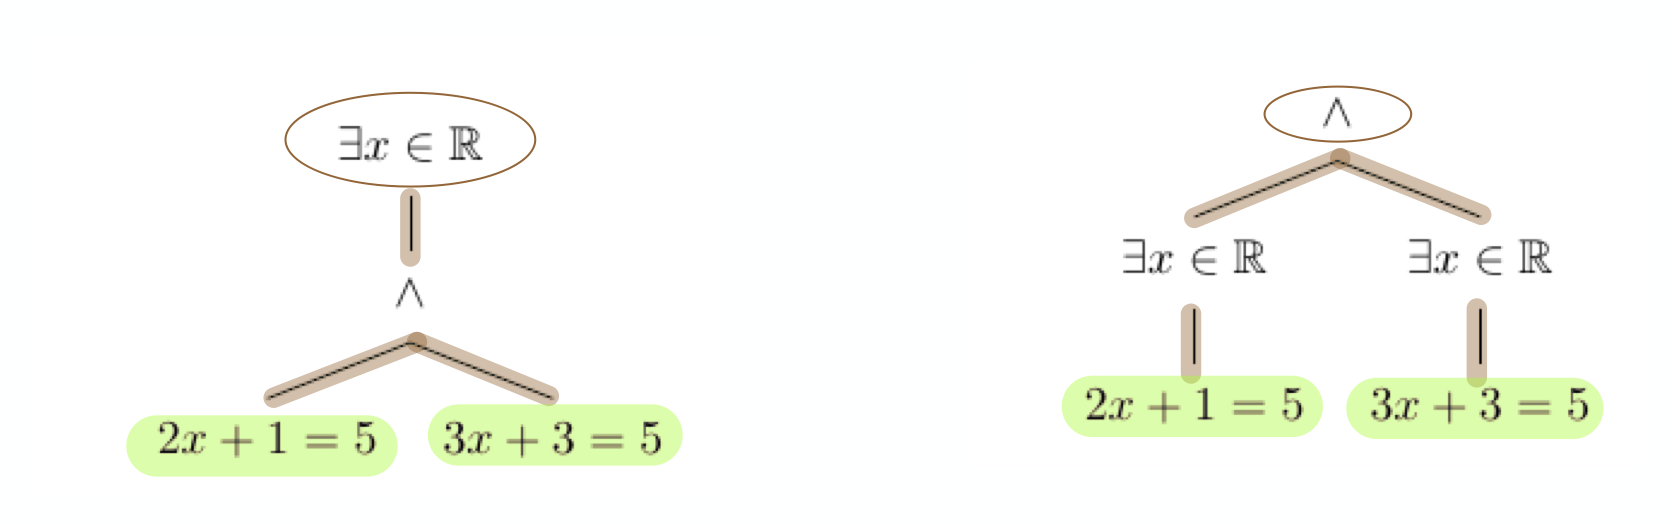
\includegraphics[scale = 0.4]{trees}

Here the root is circled, the branches are colored brown, and the leaves are colored green.

Comparing these two we see that in (1) the existential quantification of $x$ applies to both statements $2x+1 = 5$ and $3x+3  = 5$.  We would say that both instances of $x$ are within the \index{scope}\textbf{scope} of this existential quantifier.  However, in (2) the scope of the exitential quantifier on the left branch only includes the $x$ in $2x+1  = 5$, while the scope of the existential quantifier on the right branch only includes the $x$ in $3x+3 = 5$.

\begin{example}
	Assume that $p$ is a proposition while $A$, $B$, and $C$ are predicates. The syntax tree for 
	
	\[
	\exists x :[( P \wedge A(x)) \wedge ( \forall y( B(x) \wedge C(x,y) ))]
	\]
	
	is
	
	\begin{center}
		\begin{forest}
			[\(\exists x\)[\(\wedge\)[\(\wedge\)[\(P\)][\(A(x)\)]][\(\forall y \)[\(\wedge\)[\(B(x)\)][\({C(x,y)}\)]]]]]
		\end{forest}
	\end{center}
	
	The two dimensional layout of the tree makes some features of the expression easier to parse than when we leave it as a one dimensional written expression.
\end{example}

\begin{xca}
	Build a syntax tree for each of the following statements.  Assume that $p$, $q$, and $r$ are propositions and $A$, $B$, and $C$ are predicates.  Matching parenthesis can be a struggle:  this is part of the reason why trees can be a useful way of writing these expressions.  Then categorize the sentence according to its root node.
	
	\begin{enumerate}
		\item $\forall x:  p \wedge \exists y :(A(x,y) \wedge B(x)))$
		\item $p \wedge (q \wedge \exists t: (B(t,t)) )$
		\item $\forall x: ( \exists y (A(x,y)) \wedge \forall y: (C(x,y)))$
	\end{enumerate}
\end{xca}


\begin{solutions}
	\begin{enumerate}
		\item $\forall x:  (p \wedge \exists y: (A(x,y) \wedge B(x)))$
		
		\begin{center}
			\begin{forest}
				[\(\forall x\)[\(\wedge\)[\(p\)][\(\exists y\)[\(\wedge\)[\({A(x,y)}\)][\(B(x)\)]]]]]
			\end{forest}
		\end{center}
	

	
		\item $p \wedge (q \wedge \exists t: (B(t,t)) )$
		
		\begin{center}
			\begin{forest}
				[\(\wedge\)[\(p\)][\(\wedge\)[\(q\)][\(\exists t\)[\({B(t,t)}\)]]]]
			\end{forest}
		
		\end{center}
		\item $\forall x: ( \exists y (A(x,y)) \wedge \forall y (C(x,y)))$
		
		\begin{center}
			\begin{forest}
				[\(\forall x\)[\(\wedge\)[\(\exists y\)[\({A(x,y)}\)]][\(\forall y\)[\({C(x,y)}\)]]]]
			\end{forest}
	
		\end{center}
		
	\end{enumerate}
\end{solutions}

\begin{xca}
	Consider the syntax tree
	
	\begin{center}
		\begin{forest}
			[$\forall x$[$\wedge$[$\exists y$[${A(x,y)}$]][$\forall y$[$\wedge$[$p$][${B(x,y)}$]]]]]
		\end{forest}
	\end{center}
	
	Indicate all variables which are in the scope of $\forall y$.  Then convert this syntax tree to a linear string with appropriate parentheses. 
	
\end{xca}

\begin{solutions}
	The only variable within the scope of $\forall y$ is the $y$ in $B(x,y)$.
	
	We can write this proposition on one line as
	
	\[
	\forall x: (  (\exists y: ( A(x,y)))  \wedge (\forall y: ( p \wedge  B(x,y)))  )
	\]
	
\end{solutions}

\section{Natural Deduction Proof Outlines}

We have seen that we can make the logical structure of mathematical statements clearer by translating them into symbolic form.  That is to say, if we declare the meaning of sentences like $p$, $q$, $r$,  and predicates like $A(x)$,  $B(x)$,  $C(x,y)$, then we can use the logical connectives $\wedge$, $\implies$, $\bi$, $\neg$, $\vee$ and the quantifiers $\forall$ and $\exists$ to translate mathematical statements in English into more formal and precise statements using these symbols.

For example, if we let $E(x)$ be the predicate ``$x$ is even'', then we can translate the English mathematical sentence 

{ \begin{center}
		``The product of any two even numbers is even.''
		\end{center}
}

into a symbolic form where its logical structure is more apparent:

$$
\forall x \in \Z \, \forall y \in \Z \left( E(x) \wedge E(y) \implies E(x+y) \right)
$$

or as a syntax tree:

\begin{center}
\begin{forest}
	[$\forall x \in \Z$[$\forall y \in \Z$[$\implies$[$\wedge$[$E(x)$][$E(y)$]][$E(x+y)$]]]
]
\end{forest}
\end{center}

We will see how to use this logical structure to make a ``Natural Deduction Proof Outline''  for the theorem.  We will generate this outline recursively, moving down the tree.  Proving theorems in mathematics requires considerable creativity, but that creativity often lives in the ``blank spaces'' of this outline, not in the structure of the outline itself.  For each of the five connectives, and two quantifiers, we will use our elimination and introduction rules to guide us in crafting the outline.

Now lets see how to make a proof outline for 

$$
\forall x \in \Z \, \forall y \in \Z \left( E(x) \wedge E(y) \implies E(x+y) \right)
$$

\begin{center}
	\begin{forest}
		[$\forall x \in \Z$[$\forall y \in \Z$[$\implies$[$\wedge$[$E(x)$][$E(y)$]][$E(x+y)$]]]
		]
	\end{forest}
\end{center}

The root of the tree is $\forall x \in \Z$, so (looking at the introduction rule for universal quantifiers) our argument should look like this:

\begin{fitch}
		\textrm{Let $x_1 \in \Z$ be arbitrary} & start $\forall$-intro\\
		\textrm{Prove $\forall y \in \Z \left( E(x_1) \wedge E(y) \implies E(x_1+y) \right)$}\\
	\end{fitch}

How do we prove $\forall y \in \Z \left( E(x_1) \wedge E(y) \implies E(x_1+y) \right)$?  We make a syntax tree and follow the table!

\begin{center}
	\begin{forest}
		[$\forall y \in \Z$[$\implies$[$\wedge$[$E(x_1)$][$E(y)$]][$E(x_1+y)$]]]
	\end{forest}
\end{center}

The root of this tree is also a universal quantifier.  So our argument now looks like this:

\begin{fitch}
	\textrm{Let $x_1 \in \Z$ be arbitrary} & start $\forall$-intro\\
	\textrm{Let $y_1 \in \Z$ be arbitrary}& start $\forall$-intro\\ 
	\textrm{Prove $\left( E(x_1) \wedge E(y_1) \implies E(x_1+y_1) \right)$}\\
\end{fitch}

Now $\left( E(x_1) \wedge E(y_1) \implies E(x_1+y_1) \right)$ has tree

\begin{center}
	\begin{forest}
	[$\implies$[$\wedge$[$E(x_1)$][$E(y)$]][$E(x_1+y)$]]
	\end{forest}
\end{center}

whose root node is implication.  Following the introduction rule for implication, we have

\begin{fitch}
	\textrm{Let $x_1 \in \Z$ be arbitrary}& start $\forall$-intro\\
	\textrm{Let $y_1 \in \Z$ be arbitrary}& start $\forall$-intro\\ 
	\textrm{Assume $E(x_1) \wedge E(y_1)$} & start $\implies$-intro\\
	\fa \textrm{ Prove  $E(x_1+y_1)$}\\
\end{fitch}

Let's use the conjunction elimination rule to spell out exactly what we are allowed to use in our argument:

\begin{fitch}
	\textrm{Let $x_1 \in \Z$ be arbitrary}& start $\forall$-intro\\
	\textrm{Let $y_1 \in \Z$ be arbitrary}& start $\forall$-intro\\ 
	\textrm{Assume $E(x_1) \wedge E(y_1)$}& start $\implies$-intro\\
	\fa E(x_1) & $\wedge$-elim (left)\\
	\fa E(y_1) & $\wedge$-elim (right)\\
	\fa \textrm{Prove  $E(x_1+y_1)$}\\
\end{fitch}

This is a natural deduction outline for the theorem!

Let's do a few more examples which are entirely abstract.

\begin{example}
		We will make a natural deduction outline for a theorem of the form
		
		\[
		\forall t: \exists s: [ A(t,s) \bi (P(t) \vee Q(s))]
		\]
		
		First we make the syntax tree:
		
		\begin{center}
				\begin{forest}
						[$\forall t$ [ $\exists s$ [$\bi$ [${A(s,t)}$][$\vee$[$P(t)$][$Q(s)$]]] ]]
					\end{forest}
			\end{center}


We build the proof outline in stages.  The current root is universal quantification.

\begin{fitch*}
		\textrm{Let $t_1$ be arbitrary.} & start $\forall$-intro\\
		\textrm{Prove $\exists s [ A(t_1,s) \bi (P(t_1) \vee Q(s))]$}
	\end{fitch*}

The root of what we are trying to prove is now existential quantification.

\begin{fitch*}
	\textrm{Let $t_1$ be arbitrary.}& start $\forall$-intro\\
	\textrm{Construct a candidate $s_1$ (which might depend on the choice of $t_1$).} & start $\exists$-intro\\
	\textrm{Prove $A(t_1,s_1) \bi (P(t_1) \vee Q(s_1))$}\\
\end{fitch*}

The root of what we are trying to prove is now a biconditional.

\begin{fitch}
	\textrm{Let $t_1$ be arbitrary.}& start $\forall$-intro\\
\textrm{Construct a candidate $s_1$ (which might depend on the choice of $t_1$).} & start $\exists$-intro\\
	\textrm{Assume $A(t_1,s_1)$} & forward $\implies$-intro\\
	\fa \textrm{Prove $P(t_1) \vee Q(s_1)$}\\
	\textrm{Assume $P(t_1) \vee Q(s_1)$} & backwards $\implies$-intro\\
	\fa \textrm{Prove $A(t_1,s_1)$}
\end{fitch}

\medskip

We have work to do in line $4$.  The objective in line $4$ is a disjunction, so we need to either prove one or the other.  Since we have no idea what these propositions actually are, we cannot decide which one to prove in this case.  So we will just choose one for illustrative purposes.

We can also spell out how we will use the disjunction in line $5$.  This becomes a case analysis, where we need to prove $A(t_1,s_1)$ in both cases.  

\begin{fitch}
	\textrm{Let $t_1$ be arbitrary.}& start $\forall$-intro\\
\textrm{Construct a candidate $s_1$ ( might depend on $t_1$).} & start $\exists$-intro\\
\textrm{Assume $A(t_1,s_1)$} & forward $\bi$-intro\\
	\fa \textrm{Prove $P(t_1)$}\\
	\fa P(t_1) \vee Q(s_1) & $\vee$-intro (left)\\
	\textrm{Assume $P(t_1) \vee Q(s_1)$} & backwards $\bi$-intro\\
	\fa \textrm{Case 1:  Assume $P(t_1)$} & $\vee$-elim case 1\\
	\fa \fa \textrm{Prove $A(t_1,s_1)$}\\
	\fa \textrm{Case 2:  Assume $Q(s_1)$}& $\vee$-elim case 2\\
    \fa \fa \textrm{Prove $A(t_1,s_1)$}\\
    \fa A(t_1,s_1) & $\vee$-elim, 7, 9\\
    A(t_1,s_1) \bi (P(t_1) \vee Q(s_1)) & finish $\bi$-intro 3, 6\\
    \exists s: A(t_1,s) \bi (P(t_1) \vee Q(s)) & finish $\exists$-intro with $s=s_1$, 2\\
	\forall t: \exists s: [ A(t,s) \bi (P(t) \vee Q(s))] & finish $\forall$-intro, 1
\end{fitch}

\textbf{Note}:  line $4$ could have instead said ``Prove $Q(s_1)$'' if that was more appropriate in proving the particular statement of this form we were grappling with.

This proof outline is now complete!

	\end{example}

Lets do another example.  This time we will be less methodical:  you should practice translating from the sentence, to the tree, to the proof outline without using the table.  These elimination and introduction strategies should become fully integrated into your understanding of what the connectives and quantifiers mean.

\begin{example}
		\[
		\forall x:  [ P(x) \implies (\exists y: \neg Q(x,y))]
		\]
	\end{example}

\begin{center}
		\begin{forest}
				[$\forall x$ [$\implies$ [$P(x)$][$\exists y$ [$\neg$ [${Q(x,y)}$]]]]]
			\end{forest}
	\end{center}

\begin{fitch}
		\textrm{Let $x_1$ be arbitrary.} & start $\forall$-intro\\
		\textrm{Assume $P(x_1)$.} & start $\implies$-intro\\
		\fa \textrm{Construct a candidate $y_1$ ( might depend on $x_1$)} & start $\exists$-intro\\
		\fa \textrm{Assume $Q(x_1,y_1)$} & start $\neg$ intro\\
		\fa \fa \textrm{Derive an absurdity (Prove $\bot$).}\\
		\fa \neg Q(x_1,y_1) & finish $\neg$ intro, 4\\
		\fa \exists y : Q(x_1,y) & finish $\exists$ -intro with $y = y_1$, 3\\
		P(x_1) \implies \exists y : Q(x_1,y) & finish $\implies$-intro, 2\\
			\forall x:  [ P(x) \implies (\exists y: \neg Q(x,y))] & finish $\forall$-intro, 1
	\end{fitch}


\begin{example}
		\[
		(\neg \forall x: P(x)) \wedge (\exists x: Q(x))
		\]


\begin{center}
		\begin{forest}
				[$\wedge$[$\neg$[$\forall x$[$P(x)$]]][$\exists x$[$Q(x)$]]]
			\end{forest}
	\end{center}

\begin{fitch}
		\textrm{Assume $\forall x: P(x)$} & start $\neg$ intro\\
		\fa \textrm{Can use that $P(x_1)$ is true for any $x_1$ we choose.} & $\forall$-elim\\
		\fa \textrm{Derive an absurdity.}\\
		\neg  \forall x: P(x) & finish $\neg$ intro, 1\\
		\textrm{Construct a candidate $x_2$.} & start $\exists$-intro\\
		\textrm{Prove $Q(x_2)$.} & finish $\exists$-intro, 5\\
				(\neg \forall x: P(x)) \wedge (\exists x: Q(x)) & $\wedge$-intro, 4, 6
	\end{fitch}
	\end{example}

\section{Proving some more complicated theorems}

We can now construct proof outlines for arbitrary sentences!  For the rest of this course we will be focused on proving theorems about mathematical objects of interest.  Here is a sample of the kinds of theorems we will prove:

\begin{enumerate}
		\item If $x$ is a real number then $x^2 = 1$ if and only if $x=1$ or $x=-1$.
		\item If $a$ is odd, and $b$ is odd, then $a+b$ is even.
		\item For every positive real number $x$, there is a real number $y$ so that if $t$ is a real number with $0<t<y$ then $0<t^2<x$.
\end{enumerate}

We did already prove theorems which were this complicated in Chapter 2.  The tools of this chapter (abstract syntax trees and natural deduction proof outlines) only exist to make it a more systematic process.  It takes any guesswork out of knowing exactly how to structure your argument.

Let's create proof outlines for each of these. 
\medskip

\begin{theorem}
		If $x$ is a real number then $x^2 = 1$ if and only if $x=1$ or $x=-1$.
	\end{theorem}
	
	You probably learned this theorem in high school algebra.  It is the real reason you put $\pm$ signs when you take square roots.  Even though you know this theorem is true, and use it frequently, you have probably never seen a proof.  
	
	Let's prove it!

We can translate this statement into symbolic logic as follows:

\[
\forall x \in \mathbb{R} : [ ({x^2 = 1}) \iff [({x=1}) \vee ({x=-1})] ]
\]

The syntax tree is

\begin{center}
		\begin{forest}
				[\(\forall x \in \mathbb{R}\)[\(\iff\)[\({x^2 = 1}\)][\(\vee\)[\({x=1}\)][\({x=-1}\)]]]]
			\end{forest}
	\end{center}


To construct the proof outline, we move recursively down the tree.  I will do this in \textbf{excruciating} detail.  You want to get to the point where you can easily write down the proof outline without working methodically like this.

The root node is a universal quantifier, so we start with that proof outline.

\begin{fitch}
	\textrm{Let $a \in \mathbb{R}$ be arbitrary.} & start $\forall$-intro\\
	\textrm{Prove $({a^2 = 1}) \iff [({a=1}) \vee ({a=-1})]$ is true. }
	\end{fitch}

The statement in line 2 is a biconditional, so to prove it we need to argue the forwards and backwards implications:

\begin{fitch}
	\textrm{Let $a \in \mathbb{R}$ be arbitrary.}& start $\forall$-intro\\
	\textrm{Assume $a^2 = 1$ is true.} & forwards $\bi$-intro\\
	\fa \textrm{Prove $(a=1) \vee (a=-1)$ is true.}\\
	\textrm{Assume $(a=1) \vee (a=-1)$ is true.} & backwards $\bi$-intro\\
	\fa \textrm{Prove $a^2 = 1$ is true.}
\end{fitch}

In the forwards part since we know that every real number is either positive, negative, or $0$, we can initiate a case analysis depending on the status of $a$.   

In the backwards part we use a case analysis as well.

\begin{fitch}
	\textrm{Let $a \in \mathbb{R}$ be arbitrary.}& start $\forall$-intro\\
	\textrm{Assume $a^2 = 1$ is true.} & forwards $\bi$-intro\\
		\fa \textrm{Case 1: Assume $a > 0$} & $\vee$-elim\\
			\fa \fa \textrm{Argue that $(a=1) \vee (a=-1)$}\\
		\fa \textrm{Case 2: Assume $a < 0$} & $\vee$-elim\\
			\fa \fa \textrm{Argue that $(a=1) \vee (a=-1)$}\\
		\fa \textrm{Case 3: Assume $a = 0$}& $\vee$-elim\\
			\fa \fa \textrm{Argue that $(a=1) \vee (a=-1)$}\\
	\textrm{Assume $(a=1) \vee (a=-1)$ is true.}& backwards $\bi$-intro\\
		\fa  \textrm{Case 1: Assume $a=1$} & $\vee$-elim case 1\\
		\fa \fa \textrm{Argue $a^2 = 1$ is true.}\\
		\fa  \textrm{Case 2: Assume $a=-1$} & $\vee$-elim case 2\\
		\fa \fa \textrm{Argue $a^2 = 1$ is true.}
\end{fitch}

To argue the disjunctions on lines 4, 6, and 8, we will need to prove either the left or right disjunct.  Looking at what case I am in, I have made a judicious choice.  To argue that $a^2=1$ in line 10, we will need to \textbf{use} the disjunction we assumed in line 9.  This is another case analysis:

\begin{fitch}
	\textrm{Let $a \in \mathbb{R}$ be arbitrary.}& start $\forall$-intro\\
	\textrm{Assume $a^2 = 1$ is true.} & forwards $\bi$-intro\\
	\fa \textrm{Case 1: Assume $a > 0$} & $\vee$-elim\\
	\fa \fa  \textrm{Argue that $a=1$}\\
	\fa \fa \textrm{Conclude that $(a=1) \vee (a=-1)$} &$\vee$-intro left\\
	\fa \textrm{Case 2: Assume $a < 0$} &$\vee$-elim\\
	\fa \fa  \textrm{Argue that $a=-1$}\\
	\fa \fa \textrm{Conclude that $(a=1) \vee (a=-1)$} &$\vee$-intro right\\
	\fa \textrm{Case 3: Assume $a = 0$} &$\vee$-elim\\
	\fa \fa  \textrm{Argue that $a=1$}\\
	\fa \fa \textrm{Conclude that $(a=1)  \vee (a=-1)$} & $\vee$-intro left\\
	\textrm{Assume $(a=1) \vee (a=-1)$ is true.}& backwards $\bi$-intro\\
\fa  \textrm{Case 1: Assume $a=1$} & $\vee$-elim case 1\\
\fa \fa \textrm{Argue $a^2 = 1$ is true.}\\
\fa  \textrm{Case 2: Assume $a=-1$} & $\vee$-elim case 2\\
\fa \fa \textrm{Argue $a^2 = 1$ is true.}
\end{fitch}


This is the complete proof outline!

We can now fill in the remaining arguments to have a proof of the theorem:

\begin{fitch}
	\textrm{Let $a \in \mathbb{R}$ be arbitrary.}& start $\forall$-intro\\
	\textrm{Assume $a^2 = 1$ is true.} & forwards $\bi$-intro\\
	\fa \textrm{Case 1: Assume $a > 0$} & $\vee$-elim\\
	\fa \fa a^2-1 = 0\\
	\fa \fa (a-1)(a+1)=0\\
	\fa \fa a-1 = 0 & note: $a+1>1$ so $a+1 \neq 0$.\\
	\fa \fa  a = 1\\
	\fa \fa \textrm{Conclude that $(a=1) \vee (a=-1)$} &$\vee$-intro left\\
	\fa \textrm{Case 2: Assume $a < 0$} &$\vee$-elim\\
	\fa \fa a^2-1 = 0\\
\fa \fa (a-1)(a+1)=0\\
\fa \fa a+1 = 0 & note: $a-1<-1$ so $a-1 \neq 0$.\\
\fa \fa  a = -1\\
\fa \fa \textrm{Conclude that $(a=1) \vee (a=-1)$} &$\vee$-intro right\\
	\fa \textrm{Case 3: Assume $a = 0$} &$\vee$-elim\\
	\fa \fa  0^2 = 1\\
	\fa \fa 0 = 1\\
	\fa \fa \bot\\
	\fa \fa \textrm{Conclude that $(a=1)  \vee (a=-1)$} & principle of explosion\\
	\fa (a=1)  \vee (a=-1) & $\vee$-elim 3, 9, 15\\
	\textrm{Assume $(a=1) \vee (a=-1)$ is true.}& backwards $\bi$-intro\\
	\fa  \textrm{Case 1: Assume $a=1$} & $\vee$-elim case 1\\
	\fa \fa a^2 = 1\\
	\fa  \textrm{Case 2: Assume $a=-1$} & $\vee$-elim case 2\\
	\fa \fa a^2 = 1\\
	\fa a^2 = 1 & $\vee$-intro 23, 25\\
	\left[ ({x^2 = 1}) \iff [({x=1}) \vee ({x=-1})] \right ] & finish $\bi$-intro, 2, 21\\
	\forall x \in \mathbb{R} : [ ({x^2 = 1}) \iff [({x=1}) \vee ({x=-1})] ] & finish $\forall$ -intro, 1
\end{fitch}

\newpage
Paragraph Proof:

Let $x \in \R$ be chosen arbitrarily.

If $x^2 = 1$ then  $x^2-1=0$, so $(x-1)(x+1)=0$.

If $x$ is positive then $x+1$ is invertible, so $x-1=0$, so $x=1$.
If $x$ is negative then $x-1$ is invertible, so $x+1=0$, so $x=-1$.
$x$ cannot be $0$ since $0^2 \neq 1$.

On the other hand, if $x=1$ or $x=-1$ we can see immediately that $x^2 =1$.

So $x^2 = 1$ if and only if $x=1$ or $x=-1$.



\begin{theorem}
	If $a$ is odd, and $b$ is odd, then $a+b$ is even.
	\end{theorem}

	We can translate this statement into symbolic logic as follows:
	
	$$
	\forall a \in \Z \,\forall b \in \Z ((\textrm{$a$ is odd} \wedge \textrm{$b$ is odd}) \implies \textrm{$a+b$ is even})
	$$

The syntax tree is

\begin{center}
	\begin{forest}
			[$\forall a \in \Z$[$\forall b \in \Z$[$\implies$ [$\wedge$[$a$ is odd][$b$ is odd]][$a+b$ is even]]]]
		\end{forest}
	\end{center}

To construct the proof outline, we move recursively down the tree.  Just like in the last proof, I will do this very methodically so that you can benefit from seeing the process in detail.

The root node is a universal quantifier, so we start with that proof outline.

\begin{fitch}
	\textrm{Let $a_1 \in \Z$ be arbitrary.} & start $\forall$-intro\\
	\textrm{ $\forall b \in \Z ((\textrm{$a_1$ is odd} \wedge \textrm{$b$ is odd}) \implies \textrm{$a_1+b$ is even})$}
	\end{fitch} 

How do we argue line 2?  We replace the statement to be proved in line 2 with its proof outline!  Line 2 is also a universally quantified sentence, so we use the corresponding proof outline (being careful not to create variable name conflicts).

\begin{fitch}
	\textrm{Let $a_1 \in \Z$ be arbitrary.}& start $\forall$-intro\\
	\textrm{Let $b_1 \in \Z$ be arbitrary.}& start $\forall$-intro\\
	\textrm{Prove $(\textrm{$a_1$ is odd} \wedge \textrm{$b_1$ is odd}) \implies \textrm{$a_1+b_1$ is even}$}\\
\end{fitch} 

Now line 3 is an implication

\begin{fitch}
	\textrm{Let $a_1 \in \Z$ be arbitrary.}& start $\forall$-intro\\
	\textrm{Let $b_1 \in \Z$ be arbitrary.}& start $\forall$-intro\\
	\textrm{Assume $( \textrm{$a_1$ is odd} \wedge \textrm{$b_1$ is odd}) $} & start $\implies$-intro \\
	\fa \textrm{Argue that $a_1+b_1$ is even.}\\
\end{fitch} 

Each of these proof outlines is useful as a different level of ``granularity" of the proof.  Maybe this proof outline is enough for me to get to work.  Maybe not, and I need more detail.  If I need more detail, I could spell out what ``odd'' and ``even'' mean, and continue to expand the proof outline further.  For instance  ``$a_1+b_1$ is even'' means $\exists n \in \Z:  a_1+b_1 = 2n$.

\begin{fitch}
	\textrm{Let $a_1 \in \Z$ be arbitrary.}& start $\forall$-intro\\
\textrm{Let $b_1 \in \Z$ be arbitrary.}& start $\forall$-intro\\
\textrm{Assume $( \textrm{$a_1$ is odd} \wedge \textrm{$b_1$ is odd}) $} & start $\implies$-intro \\
	\fa \textrm{Argue that $\exists n \in \Z, \, a_1+b_1 = 2n$ is true.}\\
\end{fitch} 

Then we could further expand line 4 by using the proof outline for existential quantification.  Actually constructing this $n$ would require us to use what we know about $a_1$ and $b_1$.

Here is a complete proof outline:

\begin{fitch}
	\textrm{Let $a_1 \in \Z$ be arbitrary.}& start $\forall$-intro\\
\textrm{Let $b_1 \in \Z$ be arbitrary.}& start $\forall$-intro\\
\textrm{Assume $( \textrm{$a_1$ is odd} \wedge \textrm{$b_1$ is odd}) $} & start $\implies$-intro \\
	\fa \textrm{We know $\exists k, \, a_1 = 2k+1$. } & Def. of odd\\
	\fa  \textrm{Let $k_1\in \Z$ satisfy $a_1 = 2k_1+1$  }. & $\exists$-elim\\
	\fa \textrm{We know $\exists k \in \Z:  b_1 = 2k+1$.} & Def. of odd\\
	\fa \textrm{Let $k_2\in \Z$ satisfy $b_1 = 2k_2+1$.}& $\exists$-elim\\
	\fa \textrm{Choose $n \in \mathbb{Z}$ somehow, and verify that $a_1+b_1 = 2n$}.\\
\end{fitch} 
 
 
This proof outline is now only a few steps away from being a full proof of the theorem.  The entire structure of the argument has been generated ``automatically'', and the only place left for our creative efforts is to figure out how to choose $n$.  There is no magic recipe for that:  there is a tiny spark of creativity needed.  At this point you should pause and play on some scratch paper to figure out what $n$ should be.  Note:  while we are playing, we don't have to be logical.  We are just trying to generate ideas.  We can be as wild as we want to be.  Once that wild, illogical play generates an idea, we then need to be logical and precise in confirming that the idea works. \footnote{The famous mathematician Terry Tao ``... recalls the day his aunt found him rolling around her living room floor in Melbourne with his eyes closed. He was about 23. He was trying to visualise a `mathematical transform'. `I was pretending I was the thing being transformed; it did work actually, I got some intuition from doing that.' His aunt is likely still puzzled. `Sometimes to understand something you just use whatever tools you have available.'" \cite{woo15}}

Here is what my play might look like:

\begin{itemize}
		\item Hmm, I need to show  $a_1+b_1$ equals something, but I don't know what $n$ is yet.  I am trying to choose an $n$ which works.
		\item What do I know about $a_1$ and $b_1$?
		\item Pretty much the only thing I know is that $a_1 = 2k_1+1$ and $b_1 = 2k_2+1$.
		\item Okay, so let me add those together.
		\item $(2k_1+1)+(2k_2+1) = 2k_1+2k_2+2$.
		\item Hmm, I want 2 times something, but what I have is just a bunch of  stuff added together.
		\item OH! I could undistribute the common factor of 2!
		\item So $a_1+b_1 = 2(k_1+k_2+1)$.
		\item So if I choose $n = k_1+k_2+1$, I should be able to make the argument work.
	\end{itemize}

Now we can fill in the details, and produce a full proof of the theorem:

Structured Proof:

\begin{fitch}
	\textrm{Let $a_1 \in \Z$ be arbitrary.}& start $\forall$-intro\\
	\textrm{Let $b_1 \in \Z$ be arbitrary.}& start $\forall$-intro\\
	\textrm{Assume $( \textrm{$a_1$ is odd} \wedge \textrm{$b_1$ is odd}) $} & start $\implies$-intro \\
	\fa \textrm{We know $\exists k, \, a_1 = 2k+1$. } & Def. of odd\\
	\fa  \textrm{Let $k_1\in \Z$ satisfy $a_1 = 2k_1+1$  }. & $\exists$-elim\\
	\fa \textrm{We know $\exists k \in \Z:  b_1 = 2k+1$.} & Def. of odd\\
	\fa \textrm{Let $k_2\in \Z$ satisfy $b_1 = 2k_2+1$.}& $\exists$-elim\\
	\fa a_1 + b_1 = (2k_1+1)+(2k_2+1)\\
	\fa a_1 + b_1 = 2k_1+2k_2+2\\
	\fa a_1 + b_1 = 2(k_1+k_2+1)\\
	\fa \textrm{Let } n_1 = k_1+k_2+1 \in \Z\\
	\fa a_1 + b+1 = 2n_1\\
	\fa \exists n \in \Z: a_1 + b+1 = 2n & $\exists$-intro with $n = n_1$\\
	\fa a_1 + b_1 \textrm{ is even} & Def. of even.\\
	( \textrm{$a_1$ is odd} \wedge \textrm{$b_1$ is odd}) \implies \textrm{$a_1 + b_ 1$ is even} & finish $\implies $-intro, 3\\
	\forall b \in \Z: ((\textrm{$a_1$ is odd} \wedge \textrm{$b$ is odd}) \implies \textrm{$a+b$ is even}) & finish $\forall$-intro, 2\\
		\forall a \in \Z: \forall b \in \Z: ((\textrm{$a$ is odd} \wedge \textrm{$b$ is odd}) \implies \textrm{$a+b$ is even})& finish $\forall$-intro, 1
\end{fitch} 

Paragraph proof:

\begin{proof}
Let $a$ and $b$ be two odd numbers.  Then there are integers $j$ and $k$ with $a = 2k+1$ and $b=2j+1$ by definition.  Hence $a+b = 2k+1 + 2j+1 = 2 (k+j+1)$.  Since $k+j+1$ is also an integer, this shows that $a+b$ is even.
\end{proof}

Notice how much careful reasoning we usually sweep under the rug!  This does all become routine with time.  You too will eventually be comfortable with this lack of detail.


We will not be so methodical with the last theorem.  We will just present the proof outlines with some brief commentary.
 
\begin{theorem}	
	For every positive real number $x$, there is a real number $y$ so that if $t$ is a real number with $0<t<y$ then $0<t^2<x$.
	\end{theorem}


\begin{center}
		\begin{forest}
				[$\forall x \in \mathbb{R}$ [$\implies$[$x>0$][ $\exists y \in \mathbb{R}$ [ $\forall t \in \mathbb{R}$ [$\implies$ [$0<t<y$][$0<t^2<x$]] ]]]]
			\end{forest}
	\end{center}

				
		\begin{fitch}
				\textrm{Let $x_1 \in \mathbb{R}$ be arbitrary.} & start $\forall$-intro\\
				\textrm {Assume $x_1 > 0$.} & start $\implies$-intro\\
				\fa \textrm{Construct a candidate $y_1$ somehow}. &  start $\exists$-intro\\
				\fa \textrm{Let $t_1 \in \mathbb{R}$ be arbitrary.} & start $\forall$-intro\\
				\fa \textrm{Assume $0< t_1 <y_1$}. & start $\implies$-intro\\
				\fa \fa \textrm{Argue that $0<t_1^2<x_1$.}
				\fa 0< t_1 <y_1 \implies 0<t_1^2<x_1 & finish $\implies$-intro, 5\\
				\fa \forall t \in \R: 0< t <y_1 \implies 0<t^2<x_1 & finish $\forall$-intro, 4\\
				\fa \exists y \in \R: \forall t \in \R: 0< t<y \implies 0<t^2<x_1 & finish $\exists$-intro, 3\\
				x_1 > 0 \implies \exists y \in \R: \forall t \in \R: 0< t <y \implies 0<t^2<x & finish $\implies$-intro, 2\\
				\forall x: \in \R: x > 0 \implies \exists y \in \R: \forall t \in \R: 0< t <y \implies 0<t^2<x & finish $\implies$-intro, 2\\
			\end{fitch}

Commentary:

Note: There will be creativity required in choosing $y_1$ in line 3, and possibly making the argument in line 6.  You are allowed to use the assumptions in line 2 and 5 while making the argument in line 6.  Both of these assumptions are still ``active'' at line 6, because line 6 is within the scope of the both vertical bars associated with the assumptions.

\newpage

Here is a complete structured argument:

		\begin{fitch}
	\textrm{Let $x_1 \in \mathbb{R}$ be arbitrary.} & start $\forall$-intro\\
	\textrm {Assume $x_1 > 0$.} & start $\implies$-intro\\
	\fa \textrm{Choose $y_1  = \sqrt{x_1/2}$ }. &  start $\exists$-intro\\
	\fa \textrm{Let $t_1 \in \mathbb{R}$ be arbitrary.} & start $\forall$-intro\\
	\fa \textrm{Assume $0< t_1 < y_1$}. & start $\implies$-intro\\
\fa \fa \textrm{Then $0 < t_1 < \sqrt{x_1/2}$}\\
\fa \fa \textrm{So $0^2 < t_1^2 < (\sqrt{x_1/2})^2$ (since $f(x) = x^2$ is increasing on $[0,\infty)$)}\\
\fa \fa \textrm{So $0< t_1^2 < \frac{x_1}{2}$}\\
\fa \fa \textrm{Since $x_1 > 0$, $\frac{x_1}{2}< x_1$}\\
\fa \fa \textrm{So $0 < t_1^2 < x_1$}\\
	\fa 0< t_1 <y_1 \implies 0<t_1^2<x_1 & finish $\implies$-intro, 5\\
	\fa \forall t \in \R: 0< t <y_1 \implies 0<t^2<x_1 & finish $\forall$-intro, 4\\
	\fa \exists y \in \R: \forall t \in \R: 0< t<y \implies 0<t^2<x_1 & finish $\exists$-intro, 3\\
	x_1 > 0 \implies \exists y \in \R: \forall t \in \R: 0< t <y \implies 0<t^2<x & finish $\implies$-intro, 2\\
	\forall x: \in \R: x > 0 \implies \exists y \in \R: \forall t \in \R: 0< t <y \implies 0<t^2<x & finish $\implies$-intro, 2\\
\end{fitch}

Here is the paragraph proof:

\begin{proof}
Let $x$ be an arbitrarily chosen positive real number.  Let $y = \sqrt{x/2}$.  Then if $0<t<y$ we can see that

\begin{align*}
		&0 <t<y\\
		&0<t<\sqrt{x/2}\\
		&0<t^2<x/2 \textrm{ since $x^2$ is increasing on $[0,\infty)$}\\
		&0<t^2<x \textrm{ since $x/2 < x$ when $x>0$}
	\end{align*}

So for every positive real $x$ we can find a $y$ (namely $y=\sqrt{x/2}$) so that if $0<t<y$ then $0<t^2<x$.
\end{proof}


\newpage



\section{Proving Uniqueness}

If $A(x)$ is a predicate, we want to express ``There is a unique $x \in \mathcal{U}$ such that $A(x)$''.

What we really mean by this is that ``There is an $x \in \mathcal{U}$ such that $A(x)$.  Additionally, if $A(x_1)$ is true and $A(x_2)$ is true, then we must have $x_1 = x_2$.''

Symbolically:

\[
(\exists x \in \mathcal{U}: A(x)) \wedge (\forall x_1, x_2 \in \mathcal{U}: A(x_1) \wedge A(x_2) \implies x_1 = x_2  )
\]

This warrants some explanation.

Requiring that $(\exists x \in \mathcal{U}: A(x)) $ is straightforward enough:  we do want \textbf{at least} one $x \in \mathcal{U}$ which makes $A(x)$ true.

The next part is trickier.  Let's unpack the meaning of $(\forall x_1, x_2 \in \mathcal{U}: A(x_1) \wedge A(x_2) \implies x_1 = x_2  )$.

This is saying that \textbf{if} $A(x_1)$ and $A(x_2)$ are both true, then $x_1$ must be $x_2$.  This is a tricky way of saying ``only one works'' while using only the logical concepts (universal quantification, implication, equality) which we have already developed.

\begin{xca}
	Prove that there is a unique $x > 0$ such that $x^2  = 9$.
\end{xca}

\begin{proof}
		Since $3^2 = 9$ and $3 > 0$,  we can see that $\exists x > 0 : x^2 = 9$.
		
		Now let $x_1$ and $x_2$ be two witnesses to the truth of the statement.  
		
		Then $x_1^2 = x_2^2$, so (taking square roots of both sides), $|x_1| = |x_2|$.  Since both $x_1$ and $x_2$ are positive we have $x_1 = x_2$.  So this solution is unique.
	\end{proof}

\newpage

\section{L3 Homework Problems}

 These problems are \textbf{very similar} to the kinds of problems you will be expected to be able to solve to demonstrate mastery of $L3$.
 
\begin{xca}
	
	Prove each of the following statements:
	
		\begin{enumerate}
			\item $x$ is even if and only if $x+5$ is odd.
			\item If $x$ divides $y$ and $z$ divides $w$, then $xz$ divides $yz$.
			\item If $x$ is odd, then $3x^2+5x+1$ is also odd.
			\item If $n$ is even then $(-1)^n = 1$.
			\item If $x$ is even then $4 \divides n^2$.
			\item For every $b >1$ there is a unique $a \in \mathbb{R}$ with $b = \frac{a+1}{a-1}$.
			\item There exist real numbers $A$ and $B$ so that every real number $x \in \mathbb{R} - \{1,2\}$, $\frac{4x}{(x-1)(x-2)} = \frac{A}{x-1} + \frac{B}{x-2}$.
			\item (Hard one!) For every $\epsilon >0$ there exists a $\delta >0$ so that if $1<x<1+\delta$ then $3<2x+1< 3+\epsilon$.
		\end{enumerate}
\end{xca}


\begin{xca}
		In the following problems make an Abstract Syntax Tree and use it to generate a Natural Deduction Proof Outline.
	\begin{enumerate}
			\item $\exists a \in U: \exists b \in U: \forall x \in U: [  (Q(a,x) \vee Q(b,x))\implies P(a,b,x)]$
			\item $(p \wedge q) \Longleftrightarrow (r \wedge s)$
			\item $(\forall x \in U: ( \neg(R(x)))) \wedge (\exists x \in U: [ P(x) \vee Q(x)])$
			\item $(\neg p) \implies (\exists x: (A(x) \vee B(x)))$
			\item $\forall x: ((A(x) \Longleftrightarrow B(x)) \implies (\forall y: p \vee G(x,y)))$
			\item $\forall s:  \exists t: ((A(s) \wedge B(t)) \Longleftrightarrow p)$
			\item $(\forall n: A(n)) \implies [(\neg p) \vee q] $
			\item $p \Longleftrightarrow \forall k:( A(k) \wedge B(k))$
			\item $[p \vee q] \implies (\exists x: (A(x,x) \vee \neg r))$
   			\item $(p \vee q) \Longleftrightarrow (s \wedge t)$
			\item $\forall x: [(\exists y: A(x,y)) \wedge (\exists y: B(x,y))]$
			\item $ (p \vee q) \implies (s \implies t)$
		\end{enumerate}
\end{xca}


			








 % ASTs and Natural Deduction Proof Outlines.
\chapter{L4 and L5:  Quotients, Remainders, and Modular Congruence }

\section{L4:  The Quotient-Remainder Theorem}

You have hopefully become an expert at proving basic statements about parity and divisibility.  You may have been very tempted to use the concept of a \textbf{remainder} when making these kinds of arguments.  Unfortunately we have not, as yet, defined what a remainder is!  We rectify that situation in this chapter.

\begin{xca}
		Compute $953 \div 7$ as you would in elementary school to obtain a quotient and a remainder, without worrying about the precise definitions of the words ``quotient'' and ``remainder''.
	\end{xca}

\begin{solutions}
    \intlongdivision{953}{7}
    
    So $953 = 136 \cdot 7 + 1$.
    
    We say that the dividend is $953$, the divisor is $7$, the quotient is $136$ and the remainder is $1$.
    
    Notice that this usage of the term ``divisor'' is in conflict with our definition of this word!  Here (and in elementary school) it is used to just mean ``the number we are dividing by''.  It is an unfortunate reality that, even in mathematics, we sometimes have more than one meaning for a given word.  In these situations we just need to understand, from context, which meaning is intended. 
	\end{solutions}

Let us attempt to craft some definitions which we will be satisfied with.

If $n \in \mathbb{Z}$ is a dividend and $d$ is a divisor then we want to obtain a quotient $q$ and a remainder $r$.  By analogy with $953 = 136 \cdot 7 + 1$ we will want

\[
n = dq + r
\]

However, this condition is not sufficient to uniquely specify which $q$ and $r$ we are talking about!

For instance it is also true that $953 = 135 \cdot 7 + 8$ (we just ``took out one seven'').  We would not call $135$ the quotient and $8$ the remainder because $8$ is larger than $7$.   We want our remainder $r$ to satisfy $0 \leq r < d$.

So say that $n \in \mathbb{Z}$ and $d \in \mathbb{Z}^+$.  Assume that we have found integers $q_1$, $r_1$, $q_2$, and $r_2$ with

\begin{align*}
n &= q_1d + r_1 \textrm{ with $0 \leq r_1 < d$}\\
n &= q_2d + r_2 \textrm{ with $0 \leq r_2 < d$}
\end{align*}

Can we conclude that $q_1 = q_2$ and $r_1 = r_2$?  In other words, does the condition that 

\[
n = qd + r \textrm{ with $0 \leq r < d$}
\]

\textbf{uniquely} specify $q$ and $r$?

We can argue that $q_1 = q_2$ and $r_1 = r_2$ as follows:

\begin{fitch}
	\textrm{Let $n \in \mathbb{Z}$ be arbitrarily chosen.}\\
	\textrm{Let $d \in \mathbb{Z}^+$ be arbitrarily chosen.}\\
	\textrm{Let $q_1,q_2,r_1,r_2 \in \mathbb{Z}$ be chosen arbitrarily.}\\
	\textrm{Assume $n  = q_1d+r_1$ and $n = q_1d + r_2$ and $0 \leq r_1 < d$ and $0 \leq r_2 < d$}\\
	\fa  q_1d + r_1 = q_2d + r_2\\
	\fa (q_1-q_2)d = r_2 - r_1\\
	\fa |q_1 - q_2|d = |r_2 - r_1|\\
	\fa 0 \leq |r_2 - r_1| < d \textrm{ since $0 \leq r_1 < d$ and $0 \leq r_2 < d$}\\
	\fa \textrm{Assume $|r_2- r_1| \neq 0 $}\\
	\fa \fa \textrm{Then $|q_1 - q_2|d \neq 0$, so $|q_1 - q_2| \neq 0$}\\
	\fa \fa \textrm{Then $|q_1 - q_2|d  \geq d$ since $|q_1 - q_2|$ is at least $1$}\\
	\fa \fa \textrm{This is absurd:  we cannot have $|q_1 - q_2|d = |r_2 - r_1|$ when $|q_1 - q_2|d \geq d$ and $|r_2 - r_1| < d$}\\
	\fa \textrm{So $|r_2 - r_1| = 0$, which implies $r_2 = r_1$}\\
	\fa \textrm{So $(q_1 - q_2)d = 0$, which implies $q_2 = q_1$}\\
	\end{fitch}


We have justified that \textbf{if} we can find integers $q$ and $r$ so that $n = dq + r$ with $0 \leq r < d$, \textbf{then} this pair of integers is the \textbf{unique} pair which works.

We have not yet justified that it is always possible to find such a pair of integers.  The proof of this relies on something called the ``principle of mathematical induction'' which we will learn later.  So we will skip the proof for now and come back to it when we discuss mathematical induction.

Until then I ask you to (conditionally) believe the following theorem:

\begin{theorem}[Quotient-Remainder Theorem]
Let $n$ be any integer and $d$ be any positive integer. Then there are unique integers $q$ and $r$ satisfying

\[
n = qd + r \textrm{ with  $0 \leq r < d$}
\]

We call $q$ the \index{quotient} \textbf{quotient} and $r$ the \index{remainder} \textbf{remainder}.
\end{theorem}

In the programming language Python  $n/d$ will output the quotient and $n\% d$ will output the remainder.  I recommend using the following website as a calculator using these commands.  Just enter an expression (like $953/7$ or $953 \% 7$) and click ``run'':

\begin{center}
\url{http://pythonfiddle.com/}
\end{center}

Although this is not typically done in mathematics, we will also adopt these quotient and remainder \textbf{operations} in this text.

\begin{definition}
		Let $n \in \mathbb{Z}$ and $d \in \mathbb{Z}^+$.  We define $n/d  = q$ and $n \% d = r$ where $q$ and $r$ are the quotient and remainder ensured by the QR theorem.
	\end{definition}

\begin{xca}
	Calculate the quotients and remainders in each of the following situations by hand.  Then double check yourself using Python.
	\begin{enumerate}
			\item $22/4$ and $22\%4$
			\item $(-22)/4$ and $(-22)\% 4$
			\item $11/1$ and $11\%1$
			\item $11/2$, $11\%2$.
			\item $0/5$, $0\%5$.
			\item $(-452)/6$, $(-452) \% 6$.
		\end{enumerate}
	\end{xca}

\begin{solutions}
	\begin{enumerate}
		\item I can see ``immediately'' that $22 = 5(4) + 2$, so the quotient is $5$ and the remainder is $2$.
		\item This is a little tougher.  My first thought was to try to use $-5(4) =-20$, but then I realized adding a positive number to this will never give me $-22$.  So I went ``one 4 further in the negative direction" to obtain $-6(4) = -24$.  Now I see that I can add $2$ to get $-22$.
		
		Since $-22 = (-6)(4) + 2$ we have that the quotient is $-6$ and the remainder is $2$.
		\item It is clear that $11 = 11(1) + 0$, so the quotient is $11$ and the remainder is $0$.
		\item I can see that $11 = 5(2)+ 1$ so the quotient is $5$ and the remainder is $1$.  Hmm, this looks a lot like the kind of calculation I do to confirm that $11$ is odd...
		\item $0 = 0(5) + 0$ so both the quotient and remainder are $0$.
		\item Generalizing from the second problem I do long division:
		
    \intlongdivision{452}{6}
    
    So $75(6)+2= 452$, which means $75(6) = 450$, and so $(-75)(6) = -450$.  This is ``not negative enough'', so I go ``one six further'' to get $(-76)(6) = -456$.  Finally I see that I can add $4$:
    
    $-452 = (-76)(6) + 4$
    
    So the quotient is $-76$ and the remainder is $4$.
    \end{enumerate}
	\end{solutions}


We can use quotients and remainders to establish an equivalent condition for divisibility statements.

\begin{theorem}
		Let $n \in \mathbb{Z}$ and $d \in \mathbb{Z}^+$.  Then $d \divides n$ if and only if $n \% d = 0$.
	\end{theorem}

		\begin{fitch}
				\textrm{Let $n \in \mathbb{Z}$ and $d \in \mathbb{Z}^+$ be chosen arbitrarily} & $\forall$-intro\\
				\textrm{Assume $d \divides n$} & $\implies$ -intro\\
				\fa \textrm{Then there is an integer $k$ with $n = dk$}\\
				\fa \textrm{Then $n = dk + 0$}\\
				\fa \textrm{So $n \% d = 0$}\\
				\textrm{So $d \divides n$ implies $n \% d = 0$} & $\implies$- intro, (2)\\
				\textrm{Assume $ n \% d = 0$} & $\implies$-intro\\
				\fa \textrm{Then there exists an integer $k$ with $n  = kd + 0 $}\\
				\fa \textrm{So $d \divides n$}\\
				\textrm{So  $n \% d = 0$  implies $d \divides n$} & $\implies$- intro, (7)\\
				\textrm{So $n \% d = 0 \bi d \divides n$} & $\bi$-intro, (6), (10)\\
				\textrm{So $\forall n \in \Z: \forall d \in \Z^+: n \% d = 0 \bi d \divides n$} & $\forall$-intro, (1)
			\end{fitch}
		
\begin{theorem}
		For all $n \in \Z$, $n$ is even if and only if $n\%2 = 0$ and $n$ is odd if and only if $n\%2 = 1$.
	\end{theorem}

I encourage you to prove this theorem yourself!  It is very similar to the proof above.

The following theorem appears innocuous, but we actually need the QR theorem  to prove it!

\begin{theorem}
		Every integer is either even or odd.
	\end{theorem}

\begin{proof}
	
	More formally we are trying to show that
	
	\[
	\forall n \in \mathbb{Z}: \textrm{$n$ is even} \vee \textrm{$n$ is odd}
	\]
	
	We will follow the proof outline, but we will use the QR theorem to introduce a case analysis on the remainder after division by $2$.
	
	\begin{fitch}
			\textrm{Let $n \in \mathbb{Z}$ be chosen arbitrarily.} & $\forall$-intro\\
			\textrm{By the QR theorem we know $n\%2 = 0$ or $n\%2 = 1$}\\
			\textrm{Case 1:  Assume $n\%2 = 0$} & $\vee$-elim (2)\\
			\fa \textrm{Then $n$ is even}\\
			\fa \textrm{So ($n$ is even) $\vee$ ($n$ is odd)} & $\vee$-intro (4) \\
			\textrm{Case 2:  Assume $n\%2 = 1$} & $\vee$-elim (2)\\
			\fa \textrm{Then $n$ is odd}\\
			\fa \textrm{So ($n$ is even) $\vee$ ($n$ is odd) } & $\vee$-intro (7) \\
			\textrm{So ($n$ is even) $\vee$ ($n$ is odd) } & $\vee$-elim (2), (3), (6)\\
			\textrm{So } \forall n \in \mathbb{Z}: \textrm{$n$ is even} \vee \textrm{$n$ is odd} & $\forall$-intro (1)
		\end{fitch}
	
	\end{proof}

\begin{xca}
	Prove that  $n^2 - 3$ is never divisible by $5$ for any integer $n$
	
	Hint:  In your proof use QR to write $n \%5 = r$ with $r = 0,1,2,3,4$ and do a case analysis.
	\end{xca}

\newpage
				
				\begin{fitch}
					\ftag{~} \textrm{\underline{To prove:  $\forall n \in \mathbb{Z}: \neg( 5 \divides (n^2 - 3))$}}\\
						\textrm{Let $n \in \mathbb{Z}$ be chosen arbitrarily} & $\forall$-intro\\
						\textrm{Assume $5 \divides (n^2 - 3)$} & $\neg$-intro\\
						\fa \textrm{So there is an integer $k$ with $n^2 - 3 =5k$}\\
						\fa \textrm{So $n^2 \% 5 = 3$}
						\fa \textrm{By QR, $n \% 5 = r$ with $r= 0 , 1, 2,3$ or $4$}\\
						\fa \textrm{Case 1:  $r=0$} & $\vee$-intro\\
						\fa \fa \textrm{Then $n = 5q$}\\
						\fa \fa \textrm{So $n^2 \% 5 = (25q^2) \% 5 = 0$}\\
						\fa \fa \bot\\
						\fa \textrm{Case 2:  $r = 1$} & $\vee$-intro\\
						\fa \fa \textrm{Then $n = 5q + 1$}\\
						\fa \fa \textrm{So $n^2 = 25q^2 + 10q + 1$}\\
						\fa \fa \textrm{So $n^2\% 5 = 1$}\\
						\fa \fa \bot\\
						\fa \textrm{Case 3:  $r = 2$} & $\vee$-intro\\
						\fa \fa \textrm{Then $n = 5q + 2$}\\
						\fa \fa \textrm{So $n^2 = 25q^2 + 20q + 4$}\\
						\fa \fa \textrm{So $n^2 \% 5 = 4$}\\
						\fa \fa \bot\\
						\fa \textrm{Case 4:  $r = 3$} & $\vee$-intro\\
						\fa \fa \textrm{Then $n = 5q + 3$}\\
						\fa \fa \textrm{So $n^2 = 25q^2 + 30q + 5 + 4$}\\
						\fa \fa \textrm{So $n^2 \% 5 = 4$}\\
						\fa \fa \bot\\
						\fa \textrm{Case 5:  $r = 4$} & $\vee$-intro\\
						\fa \fa \textrm{Then $n = 5q + 4$}\\
						\fa \fa \textrm{So $n^2 = 25q^2 + 40q + 15 + 1$}\\
						\fa \fa \textrm{So $n^2 \% 5 = 1$}\\
						\fa \fa \bot\\
						\fa \textrm{In all cases we proved $\bot$} & $\vee$-intro lines 5, 9, 14, 19, 24\\
						\textrm{So $\neg( 5 \divides n^2 - 3)$} & $\neg$-intro, line 2\\
						\textrm{So $\forall n \in \mathbb{Z}: \neg( 5 \divides (n^2 - 3))$} & $\forall$-intro, line 1.
					\end{fitch}

\newpage

\section{L4: Homework}

\begin{xca}
	Compute each of the following by hand:
	\begin{enumerate}
		\item $44/3$
		\item $44\%3$
		\item $(-72)/5$
		\item $(-72)\%10$
		\item $11/1$
		\item $11 \%1$
		\end{enumerate}
	\end{xca}

\begin{xca}
Prove each of the following statements.  You may assume that the Quotient Remainder theorem is true.
	\begin{enumerate}
		\item If $x\%5 = 3$ and $y \%5 = 2$ then $xy \% 5 = 1$.
		\item For every integer $x$, $x^2 + x$ is even.
		\item For every integer $x$, $x(x+1)(x+2)$ is divisible by $3$.
		\item If $9 \divides x^2$ then $3 \divides x$.
	\end{enumerate}
\end{xca}
				
\section{L5: Modular Congruence}

In the last section we proved the theorem that $n^2 - 3$ is never divisible by $5$ for any integer $n$.  The proof boiled down to a case analysis on the value of $n \% 5$.  So, for the purposes of this argument, the exact value of $n$ ``didn't really matter'':  the thing that mattered was the remainder of $n$ upon division by $5$.  Since the numbers $..., -7, -2, 3, 8, 13, 18, 23, ...$  all  have a remainder of $3$ when divided by $5$, they would all be treated in the same way by the argument we gave.  In fact, we established in Case 2 of that proof that all of these numbers would have the property that if $n\%5 = 3$ then it follows that $n^2 \% 4$.

We will attempt to capture these ideas in the following definition of \textbf{modular congruence}, which is a kind of ``relaxed'' notion of equality where we consider two integers to be ``the same'' (or congruent) if they generate the same remainder when divided by some ``modulus''.

Notice that in the list $..., -7, -2, 3, 8, 13, 18, 23, ...$, the difference between any two elements is a multiple of $5$.  For instance $18-3 = 15$ and $23 - (-2) = 25$.  It makes sense that if the difference of two numbers is a multiple of $5$, then the two numbers will have the same remainder when divided by $5$.  This motivates the following definition:

\begin{definition}
		Let $m \in \Z$.  Let $a,b\in \Z$.  We will say that $a$ is congruent to $b$ modulo $m$ if  $m \divides (b-a)$.	 In this case we write $a \equiv b \mod m$.
\end{definition}

The following picture might help you to understand the definition.  

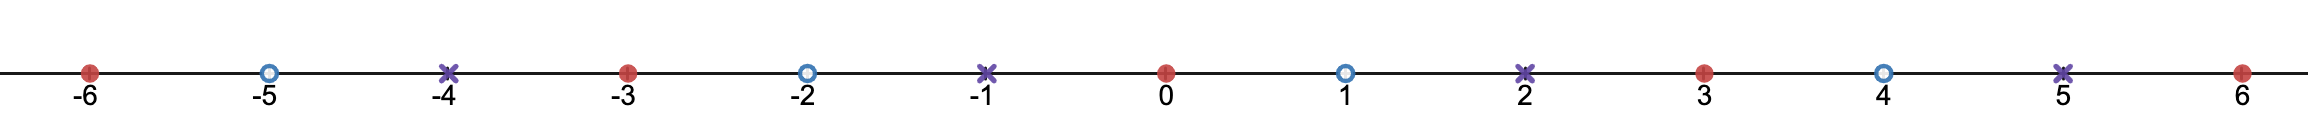
\includegraphics[scale=0.35]{mod3}

All of the numbers with the same shape are equivalent modulo $3$.  For instance, the distance from $-2$ to $4$ is $6$, which is a multiple of $3$, so $-2$ and $-4$ are equivalent modulo $3$.  For that reason they are both given blue hollow circles in this picture.
 
\begin{theorem}
Let $m$ be a positive integer.  Then $a \equiv b \mod m$ if and only if $a \% m = b \% m$.  In other words, for positive modulus $m$, two numbers are congruent modulo $m$ if and only if they have the same remainder upon division by $m$.  
\end{theorem}

\begin{fitch}
		\textrm{Let $a,b \in Z^+$, $m \in \Z^+$ be chosen arbitrarily} & $\forall$-intro\\
		\textrm{Assume  $a \equiv b \mod m$} & $\implies$-intro\\
		\fa \textrm{Then $m \divides (b-a)$}\\
		\fa \textrm{Choose a $k \in \Z^+$ with $b - a = mk$}\\
		\fa \textrm{Let $a/m = q_a$, $a \% m = r_a$, $b/m = q_b$, $b \% m = r_b$}\\
		\fa \textrm{Assume, without loss of generality, that $r_b \geq r_a$}\\
		\fa \textrm{$a = q_am+r_a$ and $b = q_bm+r_b$}\\
		\fa \textrm{$b-a = (q_b - q_a)m  + (r_b - r_a)$}\\
		\fa \textrm{$mk = (q_b - q_a)m  + (r_b - r_a)$}\\
		\fa \textrm{Since $0 \leq r_b - r_a< m$ and $m \divides(r_b - r_a)$, $r_b - r_a = 0$}\\
		\fa r_b = r_a\\
		\fa a \% m =  b \% m\\
		 a \equiv b \mod m \implies  a \% m =  b \% m & $\implies$-intro (2)\\
		\textrm{Assume $a \% m =  b \% m = r$ }  & $\implies$-intro\\
		\fa \textrm{Then $a = q_am + r$ and $b = q_bm + r$}\\
		\fa \textrm{So $b - a = (q_b - q_a)m$}\\
		\fa \textrm{So $m \divides (b-a)$}\\
		\fa \textrm{So $a \equiv b \mod m$}\\
		a \% m =  b \% m \implies a \equiv b \mod m & $\implies$-intro (14)\\
		a \% m =  b \% m \bi a \equiv b \mod m & $\bi$-intro (13), (19)\\
		\forall a,b \in \Z^+: \forall m \in \Z^+:  a \equiv b \mod m \bi a \% m =  b \% m & $\forall$-intro (1)
	\end{fitch}


I leave the proof of the following theorem to the reader.\footnote{It is \textbf{very} important that you actually prove these statements!}
\begin{theorem}
		The following basic properties of modular congruence are all true:
		
		\begin{enumerate}
			\item (Reflexivity) $a \equiv a \mod N$ for all integers $a$.
			\item (Symmetry) If $a \equiv b \mod N$ then $b \equiv a \mod N$.
			\item (Transitivity) If $a \equiv b \mod N$ and $b \equiv c \mod N$ then $a \equiv c \mod N$.
			\item (Respects addition) If $a \equiv a' \mod N$ and $b \equiv b' \mod N$ then $a+b \equiv a'+b' \mod N$.
			\item (Respects multiplication)If $a \equiv a' \mod N$ and $b \equiv b' \mod N$ then $ab \equiv a'b' \mod N$.
		\end{enumerate}
	\end{theorem}

These properties allow us to calculate remainders with surprising speed and agility, and far more efficiently that we could by using long division:

\begin{xca}
	Calculate $(73^3 + 5^9) \% 3$
	\end{xca}

\begin{solutions}
	\begin{align*}
		73^3 + 5^9 \equiv 1^3 + 2^9 \mod 3\\
		\equiv 1 + 2(2^8) \mod 3\\
		\equiv 1+2(4^4) \mod 3\\
		\equiv 1+2(1^4)\mod 3\\
		\equiv 3 \mod 3\\
		\equiv 0 \mod 3
		\end{align*}
	
Imagine how hard it would have been to calculate $73^3 + 5^9$ and then find the quotient and remainder after division by $3$!
	\end{solutions}


\section{L5: Homework}

\begin{xca}
		Use modular arithmetic to compute each of the following by hand.
	\begin{enumerate}
			\item $17^{43} + 18^{15} \% 7$
			\item $23^{12} \% 5$
			\item $23^{12} \% 10$
			\item $23^{12} \% 100$
			\item Compute the last digit of $17^{20}$.
		\end{enumerate}
	\end{xca}

\begin{xca}
		Prove each of the following statements.
		
		\begin{enumerate}
				\item (Reflexivity) $a \equiv a \mod N$ for all integers $a$.
				\item (Symmetry) If $a \equiv b \mod N$ then $b \equiv a \mod N$.
				\item (Transitivity) If $a \equiv b \mod N$ and $b \equiv c \mod N$ then $a \equiv c \mod N$.
				\item (Respects addition) If $a \equiv a' \mod N$ and $b \equiv b' \mod N$ then $a+b \equiv a'+b' \mod N$.
				\item (Respects multiplication)If $a \equiv a' \mod N$ and $b \equiv b' \mod N$ then $ab \equiv a'b' \mod N$.
			\end{enumerate}
	\end{xca}

\begin{xca}
	Prove each of the following statements.
	
	\begin{enumerate}
			\item If $a \cong b \mod n$  and $m \divides n$ then $a \cong b \mod m$.
			\item $6^n - 1$ is divisible by $5$ for all natural numbers $n$.
			\item For every $n \in \Z$ if $n \cong 3 \mod 7$ there is an $m$ in $\Z$ with $nm \cong 2 \mod 7$.
			\item If $n^2$ is congruent to $1$ mod $7$ then $n$ is either congruent to $1$ or $6$ mod $7$.  
			\item (hard) $n \cong 1 \mod 2$ if and only if $n^2 \cong 1 \mod 8$.
	\end{enumerate}
\end{xca}







 %Quotient Remainder theorem and Modular Arithmetic.
\chapter{L6: Excluded Middle}

The following statement may (or may not) seem self-evident to you:

\begin{theorem}[The Law of the Excluded Middle]
	For any statement $p$, the statement $p \vee (\neg p)$ is true. 
\end{theorem}

There is a philosophical divide in the mathematical community.  Most mathematicians think that this statement is self-evident and are happy to include excluded middle as part of their arguments.  I will call these people ``classical mathematicians''.  A smaller community, for a variety of reasons, pay attention to whether their arguments rely on this principle.  For some the reason is practical: for instance they might care about converting their proofs into programs\footnote{\url{https://en.wikipedia.org/wiki/Curry-Howard_correspondence}},or  making sure that their arguments are valid in a topos \footnote{\url{https://en.wikipedia.org/wiki/Topos}}.  Another group has more philosophical issues with excluded middle. \footnote{\url{https://en.wikipedia.org/wiki/Intuitionism}}.

The classical mathematician is comfortable with introducing excluded middle anywhere in their argument.  They would have no issue claiming ``$x = 0$  or $x \neq 0$'' as part of an argument about a real number $x$.  An intuitionist only accepts a disjunction like this if they can actually argue one of the two disjuncts.  Intuitionistic arguments are more demanding for this reason.

You might say ``What is the big deal intuitionists?  It seems obvious to me that either a real number is either $0$ or not $0$!  What problem do you have with this? ''.
More extreme uses of the Excluded Middle might give you pause.  For instance, there are some conjectures which have been open for hundreds of years (such as the famous ``Riemann Hypothesis''$ =$ RH ).  Imagine you want to argue a conjecture $C$  is true.  You give one argument if the RH is true.  Then you give a completely different argument if RH is false.  Since it is true in both cases, you argue (disjunctive elimination) that the theorem is true irrespective of the validity of the RH.  This feels unsatisfying.  We have shown that two paths lead us to the same place, but we have not justified that either path is open to us.  The intuitionist makes these distinctions very clearly.  They would accept the theorems $\textrm{RH} \implies C$ and $(\neg \textrm{RH}) \implies C$, but would not yet accept $C$ as a theorem until RH is decided.

Most mathematicians adopt a classical perspective in their work.  Whatever your philosophical or practical commitments end up being, I find that it is worthwhile to pay attention to the intuitionistic validity of your arguments.  As a matter of taste, I find that arguments which can be made intuitionistically tend to be ``cleaner'', and often provide more insight. However, for the rest of this text we will adopt a classical perspective.  We may note when a given argument is intuitionistically valid (or not) from time to time.

The next three sections in this chapter explore argument forms which are valid classically, but not intuitionistically.

\section{Proof by Contradiction}

Remember  that $\neg p$ is \textit{defined} to be $p \implies \bot$.   

So $\neg (\neg p)$ could also be written $(\neg p) \implies \bot$ or $(p \implies \bot) \implies \bot$.


It is intuitionistically valid that $p \implies [\neg (\neg p)]$:

\begin{fitch}
	\textrm{Assume $p$} & $\implies$-intro\\
	\fa \textrm{Assume $\neg p$} & $\neg$-intro\\
	\fa \fa p \wedge \neg p & $\wedge$-intro (1), (2)\\
	\fa \fa \bot & $\neg$-elim (3)\\
	\fa \neg( \neg p) & $\neg$-intro (2)\\
	 p \implies (\neg (\neg p)) & $\implies$-intro (1)
	\end{fitch}

Intuitionistically we do not have $\neg (\neg p) \implies p$, but this is classically valid.

\begin{fitch}
	\textrm{Assume $\neg (\neg p) $}\\
	\fa \textrm{$p \vee (\neg p)$}\\
	\fa \textrm{Assume $p$}\\
	\fa \fa \textrm{Then $p$}\\
	\fa \textrm{Assume $\neg p$}\\
	\fa p \wedge \neg p\\
	\fa \fa \bot \\
	\fa \fa p\\
	\fa p\\
     \neg (\neg p) \implies p
\end{fitch}

So the classical mathematician is able to make arguments using \index{proof by contradiction}\textbf{proof by contradiction}:

\begin{theorem}[Proof by Contradiction]
		In classical mathematics $p$ is equivalent to $\neg (\neg p)$, which can also be written  $\neg p \implies \bot$.
		
		In other words, to argue $p$ we may assume $\neg p$ and argue a contradiction.  This style of argument is called \index{proof by contradiction} \textbf{proof by contradiction}.
\end{theorem}

Note:  Most mathematicians only pay attention to classical logic.  We are making a distinction between ``proof of negation'' (a.k.a. negation introduction) and ``proof by contradiction''.  

This is the form of proof of negation:

\begin{fitch}
		\textrm{Assume $p$} & start $\neg$-intro\\
			\fa \textrm{Argue $\bot$}\\
			\textrm{Conclude $\neg p$.} & finish $\neg$-intro
	\end{fitch}

This is the form of proof by contradiction:

\begin{fitch}
		\textrm{Assume $\neg p$}\\
		\fa \textrm{Argue $\bot$}\\
		\textrm{Conclude $p$}.
	\end{fitch}

Most mathematicians would call both of these arguments ``proof by contradiction''.  We are being a bit more nuanced.  I learned about this distinction from a blog post of Andrej Bauer \cite{bau10}.

It is quite hard to actually come up with examples where proof by contradiction (rather than proof of negation) is actually needed.  Here is one example which relies on some knowledge of rational and irrational numbers:

\begin{example}

At least two digits in the decimal expansion of the number $\sqrt{2}$ occurs infinitely often. 

\begin{proof}
Assume to the contrary that less than two digits occur infinitely often.

If no digits occur infinitely often, then each digit occurs finitely often.  This is impossible since there are infinitely many place values to fill!  Here I am following the convention that I have ``filled in'' all of the trailing zeros.

If only one digit $j$ occurs infinitely often, then all of the other digits occur only finitely often.  Say that the last time a digit other than j appears is in the $k^{th}$ slot.  Then the decimal would be of the form $1.d_1d_2d_3\cdots d_kjjjjj...$.  However any such ``repeating'' decimal expansion is known to be rational, while $\sqrt{2}$ is known to be irrational.    Thus this also leads to a contradiction.

Therefore at least two digits in the decimal expansion of the number $\sqrt{2}$ occurs infinitely often. 
\end{proof}
	\end{example}

Note:  This proof establishes the fact that at least two digits in the decimal expansion of the number $\sqrt{2}$ occur infinitely often.  However, it gives us no clue as to \textbf{which} two digits will appear infinitely often.  

Classical mathematics is a dark art, and like any dark art it demands terrible sacrifices.  When we invoke the law of the excluded middle we are able to prove things more easily, but the price we pay is the \textbf{constructive} character of the proof.  

If we put on our intuitionist cap and try to prove the same theorem, we are now restricted to our original introduction and elimination rules without excluded middle.  That means that to prove that  there exist two digits in the decimal expansion of the number $\sqrt{2}$ which occur infinitely often we will need to give an \textbf{explicit example} of two digits (say $3$ and $7$) and then prove that these particular digits occur infinitely often.  This is much harder, but also gives us more explicit knowledge than the classical proof.

This was an example of the sacrifice we make when proving an existence theorem using proof by contradiction.  The following table summarizes the sacrifices we make when proving other types of theorems by contradiction:


\begin{table}[h]
	\centering
	\begin{tabular}{l?p{8 cm}} Type of statement
		& The sacrifice we make  using proof by contradiction\\ \hline 
		$p \vee q$ &  I know that either $p$ or $q$ is true, but I cannot tell you which one. \\ \hline
        $p \wedge q$ &  I don't have a direct argument for $p$ and $q$ independently.\\ \hline
        $\neg p$ & There is no sacrifice.  $\neg p$ is equivalent to $\neg (\neg (\neg p))$ in intuitionist logic as well.  A bit weird to do though.\\ \hline
		$p \implies q$ & If you hand me an argument that $p$ is true, I do not actually have a way to use that data to argue $q$.  All I can do is tell you that there should be such an argument. \\ \hline
		$\exists x \in U: A(x)$ &  While I know that \textbf{some} $x_1 \in U$ makes $A(x_1)$ true, I do not know how to actually show you one.\\ \hline
		$\forall x \in U: A(x)$ &  If you hand me a particular $x_1 \in U$ I don't have a direct argument that $A(x_1)$ is true.  I can only show you that assuming it is not true leads to contradiction.  In other words, whatever type of  statement $A(x_1)$ is, I will pay the associated price for that statement.\\ \hline
	\end{tabular}
\end{table}

\newpage

\section{Proof by Contraposition}

Intuitionistically, if we know $p \implies q$, we can derive $ \neg q \implies \neg p$:

\begin{fitch}
	\fj	\textrm{Assume $p \implies q$} &  $\implies$-intro\\ %1
	\fa \fh \textrm{Assume $\neg q$} & $\implies$-intro \\ %2
	\fa \fa \fh \textrm{Assume $p$} & $\neg$-intro \\ %3
	\fa \fa \fa \fa  \textrm{$q$} & $\implies$-elim (1), (3)\\ %4
	\fa \fa \fa \fa \bot & $\neg$-elim (2), (4)\\ %5
	\fa \fa \fa \neg p & $\neg$ intro, (3)\\ %6
	\fa \fa  \neg q \implies \neg p & $\implies$-intro (2), (6)\\ %7
	 \fa [ p \implies q] \implies [(\neg q) \implies (\neg q)] & $\implies$-intro (1)\\ %8
\end{fitch}

If we know $(\neg q) \implies (\neg p)$  and we accept the Law of the Excluded Middle, then we can also derive $p \implies q$:

\begin{fitch}
	\fj \textrm{Assume $(\neg q) \implies (\neg p)$ } & \\ %9
	\fa \fh \textrm{Assume $p$} & \\ %10
	\fa \fa \fa q \vee \neg q & Excluded middle \\ %11
	\fa \fa \fa \textrm{Assume $q$}  & \\ %12
	\fa \fa \fa \fa q & by (12) \\ %13
	\fa \fa \fa \textrm{Assume $\neg q$} \\  %14
	\fa \fa \fa \fa \neg p & $\implies$ elim, (9) and (14)\\ %15
	\fa \fa \fa \fa \bot & (15) and (10) \\ %16
	\fa \fa \fa \fa q & (16) and principle of explosion \\ %17
	\fa \fa \fa  q& $\vee$ elim (11), (12)--(13), and (14)--(17) \\ %18
	\fa \fa p \implies q & $\implies$ intro (10), (11)--(18)\\ %19
	\fa [(\neg q) \implies (\neg p)] \implies (p \implies q) & $\implies$ intro (9), (10)--(19)\\ %20
	 \ftag{~}{\fs [(\neg q) \implies (\neg p)] \implies [ p \implies q] } & $\bi$ introduction (1) and (20) %21
	\end{fitch}

\begin{theorem}
		The \index{Contrapositive}\textbf{contrapositive} of the implication  $p \implies q$ is the implication $(\neg q) \implies (\neg p)$ .  In classical mathematics an implication is equivalent to its contrapositive.
	\end{theorem}

Warning:  The statement $p \implies q$ is \textbf{not} equivalent to either $q \implies p$ or  $(\neg p) \implies (\neg q)$.  However, $q \implies p$ is equivalent to   $(\neg p) \implies (\neg q)$,  since the second is the contrapositive of the first.

\begin{definition}
		The \index{Converse}\textbf{converse} of the implication $p \implies q$ is the implication $q \implies p$.  The \index{Inverse}\textbf{inverse} of the implication $p \implies q$ is the implication $(\neg q) \implies (\neg q)$.  
	\end{definition}

Note:  An implication is not logically equivalent to either its converse or inverse.  However, the converse and inverse of an implication are logically equivalent to each other.  Also, while the term ``inverse'' is standard in the literature, my personal experience is that this term is not used often.  The terms ``contrapositive'' and ``converse'' are both in widespread use.

Let's see an example of how proving the contrapositive of a given implication can be easier than proving the original implication:

\begin{example}
		If $n^2$ is even, then $n$ is also even.
		
		\begin{proof}
				More formally we are saying that 
				
				\[
				\forall n \in \Z: (n^2 \textrm{ is even} \implies (n \textrm{ is even}))
				\]
				
				If we attempted to prove this directly, we might start by writing $n^2 = 2k$ for some integer $k$.  Unfortunately there is no easy way to manipulate this equation to isolate $n$ in this expression in a way that ``keeps us'' within the realm of integers.  It is much easier to prove the converse:
				
				\[
				\forall n \in \Z: (n\textrm{ is not even} \implies (n^2 \textrm{ is not even}))
				\]
				
				Since we already know that a number is not even if and only if it is odd, we can rephrase what we are now trying to prove as
				
				\[
				\forall n \in \Z: (n \textrm{ is odd} \implies (n^2 \textrm{ is odd}))
				\]
				
				At this point the proof is clear.
				
				\begin{fitch}
				\textrm{Let $n \in \Z$ be chosen arbitrarily.}\\
				\textrm{Assume $n$ is odd.}\\
				\fa \textrm{ Then we can find an integer $k$ with $n = 2k+1$}\\
				\fa \textrm{  So $n^2 = 4k^2 +4k+1 = 2(2k^2+2k) + 1$}\\
				\fa \textrm{ So $n^2$ is also odd.}
				\end{fitch}
				
			\end{proof}
	\end{example}

\newpage


\section{Proving Disjunctions using the Disjunctive Syllogism}

It is intuitionistically valid that $p \vee q$ implies $(\neg p) \implies q$:

\begin{fitch}
		\textrm{Assume $p \vee q$} & $\implies$-intro\\
		\fa \textrm{Assume $\neg p$} & $\implies$-intro\\
		\fa \fa \textrm{Case 1:  $p$ is true} & $\vee$-elim\\
		\fa \fa \fa p \wedge \neg p\\
		\fa \fa \fa \bot\\
		\fa \fa \fa q\\
		\fa \fa \textrm{Case 1:  $q$ is true} & $\vee$-elim\\
		\fa \fa \fa q\\
		\fa \fa q\\
		\fa (\neg p) \implies q\\
		(p \vee q) \implies [(\neg p) \implies q]
	\end{fitch}

Classically we also have the converse that $(\neg p) \implies q$ implies $p \vee q$:

\begin{fitch}
		\textrm{Assume $(\neg p) \implies q$}\\
		\fa p \vee (\neg p)\\
		\fa \textrm{Case 1:  $p$}\\
		\fa \fa p \vee q\\
		\fa \textrm{Case 2:  $\neg p$}\\
		\fa \fa q\\
		\fa \fa p \vee q\\
		\fa p \vee q\\
		(\neg p) \implies q \implies (p \vee q)
	\end{fitch}

so we have proven the following theorem:

\begin{theorem}
	In classical mathematics $p \vee q$ is equivalent to $(\neg p) \implies q$.  This is called the \index{disjunctive syllogism} \textbf{disjunctive syllogism}.
	\end{theorem}

So, at least in classical mathematics, we may prove a disjunction by instead proving that the negation of one disjunct implies the other.

This is a fairly normal way to reason in everyday life as well.  Most people would consider the following two sentences to have the same meaning:

\begin{itemize}
		\item You will either do your homework or you will suffer the consequences.
		\item If you do not do your homework, then you will suffer the consequences.
	\end{itemize}

The following example should be familiar from high school algebra:

\begin{xca}
	Prove that if a real number $x$ satisfies $x^2 + 5x + 6 = 0$ then either $x=-2$ or $x=-3$.
	\end{xca}


\begin{proof}
		Pick $x \in \mathbb{R}$ arbitrarily. Assume $x^2 + 5x + 6 =0$.  We want to show that either $x=-2$ or $x=-3$.
		
		So assume $x \neq -2$.
		
		Then
		
		\begin{align}
			x^2 + 5x + 6 &=0\\
			(x+2)(x+3) &=0\\
			\frac{1}{x+2} \cdot (x+2)(x+3) &=\frac{1}{x+2} \cdot 0\\
			 x + 3 = 0\\
			 x = -3
		\end{align}
	
	Note that on line $3$ we use the fact that $x \neq -2$ to utilize the multiplicative inverse of $x+2$.
	
	So if $x \neq -2$ then $x=3$.  So we can conclude either $x = -2$ or $x = -3$.
	
	Notice that we have not shown the converse of the implication (that if $x = -2$ or $x=-3$ then $x^2 +5x + 6 = 0$) although this is also true.
	\end{proof}

\newpage

\section{L6 Homework}

 These problems are \textbf{very similar} to the kinds of problems you will be expected to be able to solve to demonstrate mastery of $L6$.
 
 \begin{xca}
 		\begin{enumerate}
 			\item[]
 				\item Create the proof outline for proving each of the following theorems \textbf{by contradiction}.
 				\begin{enumerate}
 						\item $p \vee q$
 						\item $p \implies q$
 						\item $\exists x \in U: P(x)$
 					\end{enumerate}
 				\item Each of the following statements contains exactly one implication.  Rewrite that implication in contrapositive form.  Don't change anything else!
 				
 				\begin{enumerate}
 						\item $\forall x\in U: P(x) \implies (Q(x) \vee R(x)) $
 						\item $ p \implies (r \wedge \exists x \in U: P(x))$
 						\item $p \vee (q \implies r)$
 					\end{enumerate}
 				
 				\item Each of the following statements contains exactly one disjunction (``or'' statement).  Rewrite the disjunction using the disjunctive syllogism.   Don't change anything else!
 				
 				\begin{enumerate}
 						\item $(p \wedge q) \vee (\forall x: R(x))$
 						\item $(p \vee q) \implies r$
 						\item $p \implies (q \vee r)$
 					\end{enumerate}
 			\end{enumerate}
 	\end{xca}
 
 \begin{xca}
 	
 \begin{enumerate}
 	\item[]
 	\item 	 The following theorem statement contains only one implication.  Rewrite the theorem statement (in plain English) in contrapositive form, and then prove the theorem.
 	
 	\begin{quote}
 		For all integers $a,b$, and $c$, if $a^2+b^2 = c^2$ then $a$, $b$, and $c$ cannot all be odd.
 	\end{quote}
 
\item Assume $x$ and $y$ are integers with $xy \cong 3 \mod 7$.  Use a proof by contradiction to argue that $x$ is not divisible by $7$.

Note:  this will feel ``redundant'' compared to the regular proof of negation.  If this distinction is too subtle, just give the proof by negation and have a conversation with your instructor or a classmate about the difference.

\item The following theorem statement includes only one disjunction.  Rewrite the theorem statement (in plain English) using an implication instead of a disjunction.

\begin{theorem}[Euclid's Lemma]
	Let $p$ be a prime number.  Let $a,b \in \Z$.  If $p \divides ab$ then $p \divides a$ or $p \divides$ b.
	\end{theorem}

You do not need to prove the theorem, just restate it without using the words ``not'' and ``implies'' but not the word ``or''.

 	\end{enumerate}
 	\end{xca} % LEM and consequences.
%\include{L7-old-version} % Logical Equivalences from LEM.
\chapter{L7 and L8: Boolean Algebra and Truth Tables}

\section{L7: Boolean Arithmetic}
The classical mathematicians believes the law of the excluded middle: $p$ or not $p$.  There is no grey zone.  If the intuitionist cannot actually prove one of $p$ or $\neg p$, then they remain agnostic about the truth of the statement $p \vee (\neg p)$.

The ``black and white'' thinking of classical mathematics simplifies things in logic.  We can determine the truth of a compound statement, built out of atomic propositions like $p$, $q$, $r$, etc together with the  logical connectives $\wedge$, $\implies$, $\bi$, $\neg$, $\vee$ from the truth value of the atomic propositions \textbf{without} actually forming an argument!  We say that, in classical logic, these connectives are \textbf{truth functional}.

Letting $1$ stand for true and $0$ stand for false (instead of our usual $\top$ and $\bot$), we can see that 

\begin{table}[h!]
	\begin{center}
		\caption{Truth Table for conjunction}
		\begin{tabular}{c|c} 
			$p$  & $\neg p$ \\
			\hline
			$0$ & $1$ \\ 
			$0$ & $0$ \\ 
		\end{tabular}
	\end{center}
\end{table}

\begin{table}[h!]
	\begin{center}
		\caption{Truth Table for conjunction}
		\begin{tabular}{c|c|c} 
			$L$ & $R$ & $L \wedge R$ \\
			\hline
			$0$ & $0$ & $0$ \\ 
			$0$ & $1$ & $0$ \\ 
			$1$ & $0$ & $0$ \\ 
			$1$ & $1$ & $1$ \\ 
		\end{tabular}
	\end{center}
\end{table}

\begin{table}[h!]
	\begin{center}
		\caption{Truth Table for implication}
		\begin{tabular}{c|c|c} 
			$L$ & $R$ & $L \wedge R$ \\
			\hline
			$0$ & $0$ & $1$ \\ 
			$0$ & $1$ & $1$ \\ 
			$1$ & $0$ & $0$ \\ 
			$1$ & $1$ & $1$ \\ 
		\end{tabular}
	\end{center}
\end{table}

\begin{table}[h!]
	\begin{center}
		\caption{Truth Table for biconditional}
		\begin{tabular}{c|c|c} 
			$L$ & $R$ & $L \bi R$ \\
			\hline
			$0$ & $0$ & $1$ \\ 
			$0$ & $1$ & $0$ \\ 
			$1$ & $0$ & $0$ \\ 
			$1$ & $1$ & $1$ \\ 
		\end{tabular}
	\end{center}
\end{table}

\begin{table}[h!]
	\begin{center}
		\caption{Truth Table for disjunction}
		\begin{tabular}{c|c|c} 
			$L$ & $R$ & $L \wedge R$ \\
			\hline
			$0$ & $0$ & $0$ \\ 
			$0$ & $1$ & $1$ \\ 
			$1$ & $0$ & $1$ \\ 
			$1$ & $1$ & $1$ \\ 
		\end{tabular}
	\end{center}
\end{table}

\newpage

\begin{example} Evaluate the truth value of 
	$((1 \wedge (0 \implies (0 \implies 0))) \vee (1 \bi 0))$
	\end{example}

		\begin{align*}
		& ((1 \wedge (0 \implies (0 \implies 0))) \vee (1 \bi 0))\\
		 \equiv &  ((1 \wedge (0 \implies 1)) \vee 0\\
		 \equiv &  ((1 \wedge 1) \vee 0\\
		 \equiv &  1 \vee 0\\
		 \equiv & 1
	\end{align*}

You can get more practice doing this kind of ``arithmetic of logic'' here:

\begin{center}
 \url{https://infinitesque.net/logic-eval/}.
 \end{center}


\newpage

These kinds of computations are useful.

We often want the computer to execute some command depending on whether a set of different conditions are satisfied.  Consider the simple problem of instructing a computer to sum all of the numbers between $1$ and $100$ which are divisible by $2$ or $3$ but not both.

In psuedocode, we might write

\begin{lstlisting}[language=Python]
	set SUM = 0
	for k in {1, 2, 3, ..., 100}:
	If ((k%2==0) OR (k%3==0)) AND (NOT((k%2==0) AND (k%3==0))):
	SUM := SUM + k 
	return SUM
\end{lstlisting}

We cannot write functional code like this without understanding the precise truth functional behaviour of the connectives OR, AND, and NOT.

Many authors start with these truth functional definitions of the connectives and build logic up from there.  We have not chosen that path in this book primarily to keep the focus of logic on \textbf{making valid arguments}, which the truth functional approach does not do.

These kinds of computations can also be used to decide the truth value of quantified statements, but only when we are quantifying over finite sets.  The reason is that if you want to decide the truth value of a statement like $\forall x \in U: P(x)$ you can actually check all of the possible options of $U$ is finite.  However, it $U$ is infinite you cannot.

	\begin{xca}
	
	Given the following table of values for the predicate $P$, decide whether the propositions below are true or false.  Explain your reasoning.
	
	\begin{table}[h!]
		\begin{center}
			\label{tab:table1}
			\begin{tabular}{c|c|c|c|}
				$P(x,y)$ &$x=3$ & $x=4$ & $x=5$  \\
				\hline
				$y=1$    &   $0$        &     $1$       &     $1$      \\
				\hline
				$y=2$   &    $0$       &     $1$        &    $1$      \\
				\hline
				$y=3$   &    $0$       &      $0$        &   $1$       \\
				\hline
			\end{tabular}
		\end{center}
	\end{table}
	
	\begin{enumerate}
		\item $P(4,1)$
		\item $P(4,2)$
		\item $\exists y \in \{1,2,3\}: P(3,y)$
		\item $\exists y  \in \{1,2,3\}: P(4,y)$
		\item $\forall y  \in \{1,2,3\}: P(4,y)$
		\item $\forall y  \in \{1,2,3\}: P(5,y)$
		\item $\forall x  \in \{3,4,5\}: P(x, 1)$
		\item $\exists x  \in \{3,4,5\}: P(x,1)$
		\item $\exists b  \in \{3,4,5\}: P(b, 3)$
		\item $\exists t  \in \{3,4,5\}: P(t, t-2)$
		\item $\exists y  \in \{3,4,5\}: P(y,1)$
	\end{enumerate}
	
	
\end{xca}

\begin{solutions}
	
	\begin{enumerate}
		\item $P(4,1) = 1$
		\item $P(4,2) = 1 $
		\item $\exists y \in \{1,2,3\}: P(3,y) = 0$.  $P(3,1)$, $P(3,2)$, and $P(3,3)$ are all false.  So there is no value of $y$ from the set $\{1,2,3\}$ which makes $P(3,y)$ true.
		\item $\exists y  \in \{1,2,3\}: P(4,y) = 1$.  Setting $y=2$ gives $P(4,2) = 1$, so there is at least one value of $y$ from the set $\{1,2,3\}$ which makes $P(4,y)$ true.
		\item $\forall y  \in \{1,2,3\}: P(4,y) = 0$. Setting  $y = 3$ gives $P(4,3) = 0$, so $P(4,y)$ is not true for every value of $y$ in $\{1,2,3\}$ (even though it is true for some of them).
		\item $\forall y  \in \{1,2,3\}: P(5,y) = 1$.  $P(5,1)$, $P(5,2)$, and $P(5,3)$ are all true.  So the statement that $P(5,y)$ is true for every $y$ in $\{1,2,3\}$ is true.
		\item $\forall x  \in \{3,4,5\}: P(x, 1) = 0$.  When $x = 3$, $P(3, 1) = 0$, so it isn't true that $P(x,1)$ is true for all values of $x$ in \{1,2,3\}.
		\item $\exists x  \in \{3,4,5\}: P(x,1) = 1$.  $P(4,1) = 1$ for instance.
		\item $\exists b  \in \{3,4,5\}: P(b, 3) = 1$.  When $b = 5$, we obtain the true proposition $P(5,3)$.
		\item $\exists t  \in \{3,4,5\}: P(t, t-2) = 1$.  When $t = 4$, we obtain the true proposition $P(4,2)$.  
		\item $\exists y  \in \{3,4,5\}: P(y,1) = 1$.  Remember not to get caught up in variable names here!  Despite being called $y$, this variable is in the first slot.  A value of $y$ which works is $y = 4$, since $P(4,1) = 1$. 
	\end{enumerate}
	
\end{solutions} 

	\begin{xca}
	
	Given the following table of values for the predicate $P$, decide whether the propositions below are true or false.  Explain your reasoning.
	
	\begin{table}[h!]
		\begin{center}
			\label{tab:table1}
			\begin{tabular}{c|c|c|c|}
				$P(x,y)$ &$x=1$ & $x=2$ & $x=3$  \\
				\hline
				$y=1$    &   $0$        &     $1$       &     $1$      \\
				\hline
				$y=2$   &    $0$       &     $1$        &    $1$      \\
				\hline
				$y=3$   &    $0$       &      $1$        &   $0$       \\
				\hline
			\end{tabular}
		\end{center}
	\end{table}
	
	\begin{enumerate}
		\item $\exists t: P(t,t)$
		\item $\forall t: P(t,t)$
		\item $\exists a: \forall b: P(a,b)$
		\item $\exists a: \forall b: P(b,a)$
		\item $\forall t: \exists s: P(t,s)$
		\item $\forall t: \exists s: P(s,t)$
	\end{enumerate}
	
	
\end{xca}

\begin{solutions}
	\begin{enumerate}
		\item $\exists t: P(t,t)$ - This is a true.  $t = 2$ is a witness since $P(2,2) = 1$
		\item $\forall t: P(t,t)$ - This is false.  For instance, setting $t =1$, $P(1,1) = 0$.
		\item $\exists a: \forall b: P(a,b)$ - This is true.  When $a = 1$, we have the statement $\forall b: P(1,b)$.  This is a true statement since $P(1,1)$, $P(1,2)$, and $P(1,3)$ are all true.
		\item $\exists a: \forall b: P(b,a)$ - This is a false statement.  
		\begin{itemize}
			\item If we try $a = 1$, we have the statement $\forall b: P(b,1)$.  However, $P(1,1)$ is false.
			\item If we try $a = 2$, we have the statement $\forall b: P(b,2)$.  However, $P(1,2)$ is false.
			\item If we try $a = 3$, we have the statement $\forall b: P(b,3)$.  However, $P(3,3)$ is false.
		\end{itemize}
		
		So there is no value of $a$ which makes the predicate $\forall b: P(b,a)$ true.
		\item $\forall t: \exists s: P(t,s)$ - This is a false statement.  When $t  =1$, we have the proposition $\exists s: P(1,s)$.  This is false since $P(1,1)$, $P(1,2)$, and $P(1,3)$ are all false.
		\item $\forall t: \exists s: P(s,t)$  - This is a true statement.  
		
		\begin{itemize}
			\item If we try $t = 1$, we have the statement $\exists s: P(s,1)$.  There is such an $s$, namely $s = 2$ or $s = 3$.
			\item If we try $t = 2$, we have the statement $\exists s: P(s,2)$.  There is such an $s$, namely $s = 2$ or $s = 3$
			\item If we try $t = 3$, we have the statement $\exists s: P(s,3)$.  There is such an $s$, namely $s = 2$.
		\end{itemize}
	\end{enumerate}
\end{solutions}

\section{L7: Boolean Algebra}
We can use the rules we have already learned for logical equivalences to do ``algebra'' with logical expressions.

\begin{example}
		\begin{align*}
			p \vee \neg(q \vee r) & \equiv p \vee (\neg q \wedge \neg r)\\
			&\equiv (p \vee (\neg q)) \wedge (p \vee (\neg r))
			\end{align*}
	\end{example}

Here we have put the statement in \textbf{conjunctive normal form} \footnote{\url{https://en.wikipedia.org/wiki/Conjunctive_normal_form}} which you may be interested in reading more about.

Here is a more complicated example:


		\begin{align*}
		&\neg( p \vee \forall k: ( (\neg q) \implies ( \exists x: R(x, k)) ) ) \\
		&\equiv (\neg p) \wedge \neg [\forall k: ( (\neg q) \implies ( \exists x: R(x, k)) ) ]\\
		&\equiv (\neg p) \wedge  \exists k:  \neg [( (\neg q) \implies ( \exists x: R(x, k)) ) ]\\
		&\equiv (\neg p) \wedge  \exists k:    (\neg q) \wedge \neg ( \exists x: R(x, k))  \\
		&\equiv (\neg p) \wedge  \exists k:    (\neg q) \wedge   \forall x: \neg R(x, k) \\
		&\equiv \exists k \forall x (\neg p) \wedge( (\neg q) \wedge \neg R(x,k))
	\end{align*}

This is now in \textbf{prenex conjunctive normal form}\footnote{\url{https://en.wikipedia.org/wiki/Prenex_normal_form}}  which you may also be interested in reading more about.


\section{L8:  Enumerating Truth Assignments}

In this chapter we will be concerned with all the possible truth values which a proposition like $P \vee (Q \implies R)$ could take depending on the truth value of each \textbf{atomic proposition}  $P$, $Q$, and $R$ in the expression.  Figuring out all of the distinct available choices is difficult.  We could just start writing them down ``willy nilly''

\begin{table}[h!]
	\begin{center}
		\caption{``Willy Nilly'' truth assignments}
		\begin{tabular}{c|c|c} 
			$P$ & $Q$ & $R$ \\
			\hline
			$0$ & $0$ & $1$ \\ 
			$0$ & $1$ & $0$ \\ 
			$1$ & $0$ & $0$ \\ 
			$0$ & $1$ & $1$ \\ 
			$\vdots$ & $\vdots$ & $\vdots$ \\ 
		\end{tabular}
	\end{center}
\end{table}

This strategy has several shortcomings:

\begin{enumerate}
	\item It is hard to know that you have listed all possibilities.
	\item It is hard to check that you have not accidentally listed a combination more than once.
	\item Even if you get all of them exactly once, the particular ordering you come up with will not be easily reproducible in the future.
\end{enumerate}

These shortcomings indicate that we might be better off \textbf{organizing} the way we are listing these truth assignments.

Since each atomic proposition can be either true or false, we have $2$ choices for $P$.  Each of those $2$ choices for $P$ leads to $2$ choices for $Q$.  This is $4$ total so far.  Each of these $4$ assignments leads to $2$ choices for $R$, for a total of $8$ possibilities.  Let's try to list them all out in an organized, reproducible manner.  We will start by making a table with 8 rows:

\begin{table}[h!]
	\begin{center}
		\caption{Starting to organize the truth assignments}
		\begin{tabular}{c|c|c} 
			$P$ & $Q$ & $R$ \\
			\hline
			&  &  \\  \hline
			&  &  \\  \hline
			&  &  \\  \hline
			&  &  \\  \hline
			&  &  \\  \hline
			&  &  \\  \hline
			&  &  \\  \hline
			&  &  \\  \hline
		\end{tabular}
	\end{center}
\end{table}

We know that half of the assignments will have $P$ false, and the rest will have $P$ true.  We will list the false assignments first.


\begin{table}[h!]
	\begin{center}
		\caption{Sorting by $P$ first}
		\begin{tabular}{c|c|c} 
			$P$ & $Q$ & $R$ \\
			\hline
			0 &  &  \\  \hline
			0 &  &  \\  \hline
			0 &  &  \\  \hline
			0 &  &  \\  \hline
			1 &  &  \\  \hline
			1 &  &  \\  \hline
			1 &  &  \\  \hline
			1 &  &  \\  \hline
		\end{tabular}
	\end{center}
\end{table}

If $P$ is false, then there are $4$ choices.  Of these, half should have $Q = 0$ and the rest should have $Q = 1$.  Similar remarks apply if $P$ is true.


\begin{table}[h!]
	\begin{center}
		\caption{Sorting by $Q$ second}
		\begin{tabular}{c|c|c} 
			$P$ & $Q$ & $R$ \\
			\hline
			0 & 0 &  \\  \hline
			0 & 0 &  \\  \hline
			0 & 1 &  \\  \hline
			0 & 1 &  \\  \hline
			1 & 0 &  \\  \hline
			1 & 0 &  \\  \hline
			1 & 1 &  \\  \hline
			1 & 1  &  \\  \hline
		\end{tabular}
	\end{center}
\end{table}

Finally, look at the rows in groups of two.  In each group of two, the truth value of $P$ and $Q$ are identical, and we have exactly two choices for the truth value of $R$.  Let's fill those in:


\begin{table}[h!]
	\begin{center}
		\caption{Sorting by $R$ last}
		\begin{tabular}{c|c|c} 
			$P$ & $Q$ & $R$ \\
			\hline
			0 & 0 & 0  \\  \hline
			0 & 0 & 1 \\  \hline
			0 & 1 & 0 \\  \hline
			0 & 1 & 1 \\  \hline
			1 & 0 & 0 \\  \hline
			1 & 0 &  1\\  \hline
			1 & 1 &  0\\  \hline
			1 & 1  &  1 \\  \hline
		\end{tabular}
	\end{center}
\end{table}

This way of building this collection of possible truth assignments has mitigated all of our concerns about the ``willy nilly'' approach:

\begin{enumerate}
	\item It is easy to know that you have listed all possibilities.
	\item It is easy to check that you have not accidentally listed a combination more than once.
	\item This ordering is easily reproducible in the future.
\end{enumerate}


\begin{xca}
	
	Make a table showing all possible truth value assignments for $4$ atomic propositions $A$, $B$, $C$, $D$.  Use the same organizing principles we agreed on when creating the three column table.
	
\end{xca}

\begin{solutions}
	We can think of each choice of truth value for $A$, $B$, $C$ and $D$ as creating a fork in the road, doubling our number of possible ``paths''.
	
	\begin{center}
		\scalebox{0.5}{
			\begin{forest}
				[[${A = 0}$ [${B = 0}$ [${C = 0}$[${D = 0}$][${D = 1}$]][${C = 1}$[${D = 0}$][${D = 1}$]]][${B = 1}$ [${C = 0}$[${D = 0}$][${D = 1}$]][${C = 1}$[${D = 0}$][${D = 1}$]]]][ ${A = 1}$[${B = 0}$ [${C = 0}$[${D = 0}$][${D = 1}$]][${C = 1}$[${D = 0}$][${D = 1}$]]][${B = 1}$ [${C = 0}$[${D = 0}$][${D = 1}$]][${C = 1}$[${D = 0}$][${D = 1}$]]]]]
			\end{forest}
		}
	\end{center}
	
	Then reading from left to right we obtain
	
	\begin{table}[h!]
		\begin{center}
			\begin{tabular}{c|c|c|c} 
				$A$ & $B$ & $C$  & $D$ \\
				\hline
				$0$ & $0$ & $0$  & $0$ \\ \hline
				$0$ & $0$ & $0$  & $1$ \\ \hline
				$0$ & $0$ & $1$  & $0$ \\ \hline
				$0$ & $0$ & $1$  & $1$ \\ \hline
				$0$ & $1$ & $0$  & $0$ \\ \hline
				$0$ & $1$ & $0$  & $1$ \\ \hline
				$0$ & $1$ & $1$  & $0$ \\ \hline
				$0$ & $1$ & $1$  & $1$ \\ \hline
				$1$ & $0$ & $0$  & $0$ \\ \hline
				$1$ & $0$ & $0$  & $1$ \\ \hline
				$1$ & $0$ & $1$  & $0$ \\ \hline
				$1$ & $0$ & $1$  & $1$ \\ \hline
				$1$ & $1$ & $0$  & $0$ \\ \hline
				$1$ & $1$ & $0$  & $1$ \\ \hline
				$1$ & $1$ & $1$  & $0$ \\ \hline
				$1$ & $1$ & $1$  & $1$ \\ 
			\end{tabular}
		\end{center}
	\end{table}
	
\end{solutions}

These ``truth assignment tables'' bear some similarity to lists of numbers. To make these lists we are really just counting in binary!

For the purposes of reading the rest of this book, you do not need to know anything about binary or other bases.  You \textbf{do}need to be able to produce a truth assignment table for a set of atomic propositions in the way we have discussed in this section.

Understanding other bases is a rite of passage in mathematics and computer science culture.  Understanding the binary (base $2$)  and hexidecimal (base $16$) systems are important for computer scientists because (at its heart) a computer is ``really'' doing all of its computations using binary (``off"/``on'') circuitry.  So number systems based on powers of $2$ are important to computer scientists.

For these reasons, we provide an appendix on these other number systems.

\section{L8:  Tautologies and Equivalence}

\begin{xca}
	Consider the following four statements:  $P \implies Q$,  $(\neg P) \vee Q$, $P \vee (\neg Q)$, and $(\neg Q) \implies (\neg P)$. 
	
	A few entries of this table have been filled our correctly as a model.  Complete the rest of the table.
	
	\begin{table}[h!]
		\begin{center}
			\begin{tabular}{c|c|c|c|c|c|c|c} 
				$P$ & $Q$ & $\neg P$ & $\neg Q$  & $P \implies Q$ & $(\neg P) \vee Q$ &  $P \vee (\neg Q)$ & $(\neg Q) \implies (\neg P)$ \\
				\hline
				$0$& $0$ & $1$ &         &          &            &  $1$   &   \\ \hline
				$0$& $1$ &         & $0$ &          &            &            &  $1$  \\ \hline
				$1$& $0$ &         &         &  $0$ &            &            &     \\ \hline
				$1$& $1$ &         &         &          &  $1$   &            &      \\ 
			\end{tabular}
		\end{center}
	\end{table}
	
\end{xca}

\begin{solutions}
	
	\begin{table}[h!]
		\begin{center}
			\begin{tabular}{c|c|c|c|c|c|c|c} 
				$P$ & $Q$ & $\neg P$ & $\neg Q$  & $P \implies Q$ & $(\neg P) \vee Q$ &  $P \vee (\neg Q)$ & $(\neg Q) \implies (\neg P)$ \\
				\hline
				$0$& $0$ & $1$ & $1$ & $1$ & $1$ & $1$  &  $1$  \\ \hline
				$0$& $1$ & $1$ & $0$ & $1$ & $1$ & $0$  &  $1$  \\ \hline
				$1$& $0$ & $0$ & $1$ & $0$ & $0$ & $1$  &  $0$   \\ \hline
				$1$& $1$ & $0$ & $0$ & $1$ & $1$ & $1$ &  $1$    \\ 
			\end{tabular}
		\end{center}
	\end{table}
\end{solutions}

Notice that the columns for $P \implies Q$,  $(\neg P) \vee Q$, and $(\neg Q) \implies (\neg P)$ are all identical.  That means that no matter what the truth value of $P$ or $Q$, the truth value of these three expressions will always agree! 

\begin{definition}
	Two expressions involving $n$ letters (standing for atomic propositions) and the logical connectives $\wedge$, $\implies$, $\bi$, $\neg$, and $\vee$ are called \index{Truth Functionally Equivalent}\textbf{truth functionally equivalent} if the two expressions evaluate to the same truth value for all of the $2^n$ assignments of the atomic propositions.
	
	In other words, they are equivalent if when we make a truth table involving all $2^n$ rows the columns corresponding to the two expressions are identical.
	
	If $S_1$ and $S_2$ are two statements, we will write $S_1 \equiv S_2$ to indicate that they are truth functionally equivalent.
\end{definition}


\begin{definition}
	An expression $S$ involving $n$ letters (standing for atomic propositions) and the logical connectives $\wedge$, $\implies$, $\bi$, $\neg$, and $\vee$ is called a \index{Tautology}\textbf{tautology} if it is truth functionally equivalent to $T$.  
	
	Example:  $p \vee (\neg p)$ is a tautology.
	
	It is called a \index{Contradiction}\textbf{contradiction} if it is truth functionally equivalent to $F$.
	
	Example:  $p \wedge (\neg p)$ is a contradiction.
	
	It is called  \index{Conditionally True}\textbf{conditionally true} if it is neither a tautology nor a contradiction.
	
	Example:  $p \vee q$ is conditionally true since $0 \vee 0 = 0$ and $1 \vee 0 = 1$.
	
	In other words, $S$ is a tautology if its column in a truth table has only $1$, it is a contradiction if this column consists only of $0$, and it is conditionally true if there is a mix of $1$ and $0$ entries.
	
\end{definition}

Note:  We could have defined tautology first, and then defined $S_1 \equiv S_2$ if $S_1 \bi S_2$ is a tautology.  Think about why!







 % Boolean Algebra and Truth Tables
\chapter{Induction and Recursion}

\section{Introduction}

Mathematics is, in large part, the study of patterns.  Consider the following facts:

\begin{enumerate}
		\item $6^1 - 1 = 5$
		\item $6^2 - 1 = 35$
		\item $6^3 -1 = 215$
		\item $6^4 - 1 = 1295$
	\end{enumerate}

Looking at these four examples seems to suggest a pattern.  It seems that $6^n - 1$ is always a multiple of $5$.  You can continue experimenting to confirm that the pattern continues to hold.  However, no matter how many computations you do, you cannot prove that $6^n-1$ is \textit{always} divisible by $5$ this way.  Even if you test up to $6^{10000} - 1$, there is still a possibility that $6^{10001} - 1$ might not be divisible by $5$.

The ordered list of numbers $5, 35, 215, 1295, \dots$ is an example of a \textbf{sequence}.  We have a formula for this sequence $f(n) = 6^n -1$, for $n \in \{1,2,3,4, \dots\}$.  In other words, a sequence is just a function whose domain is a subset of the set of natural numbers.

In this section we will learn how to work with sequences which are presented explicitly by formulas and recursively by recurrence relations.  We will learn how to use sigma notation to work with sums of sequences.

We will learn a new method of proof called ``Mathematical Induction'' which will allow us to prove theorems about the natural numbers, including the theorem that $6^n - 1$ is always divisible by $5$.    We will also give some proof techniques which are equivalent to mathematical induction called ``strong induction'' and ``the well ordering principle''.

We will also apply mathematical induction to prove three important theorems:  the infinitude of the primes,  the quotient-remainder theorem, and the correctness of the Euclidean Algorithm.

\section{NN1 Sequences}

\begin{definition}
	Let $I$ be a set of consecutive integers.  For instance, we could have a finite set like $I = \{2,3,4,5\}$ or an infinite set like $I = \{5, 6, 7, 8, \dots\}$.  We call a function from $I$ to any set $X$ a \index{Sequence}\textbf{sequence} of elements of $X$ indexed by $I$.  The set $I$ is called the \index{Index Set}\textbf{index set} of the sequence, and the individual elements of $I$ are called \index{Index}\textbf{indices} (singular:  \textbf{index}).
\end{definition}

Note:  While it is common to use function notation for sequences (such as writing $f: \mathbb{N} \to \mathbb{R}$ defined by $f(n) = n^2$), it is also conventional to use a letter with a subscript for the index variable.  For instance, it is common to write $a_n = n^2, n \in \mathbb{N}$.  It is normal to substitute particular values into the index, as in $a_7  =49$.

One way to present a sequence is to give the index set and a formula (also called a \index{Closed Form Expression}\textbf{closed form expression}) for the value of the sequence at a generic input.

\begin{xca}
		Write the first four terms of each of the following sequences:
		
		\begin{enumerate}
				\item $a_n = n^2 -1, n \in \{4,5,6,\dots\}$
				\item $b_n = \cos(\pi n), n \in \mathbb{N}$
				\item $c_n = (-1)^n, n \in \mathbb{N}$
				\item $a_n = \frac{n(n+1)}{2}, n \in \mathbb{N}$
			\end{enumerate}
	\end{xca}

\begin{xca}
	Below are the first 4 terms of a sequence.  Try and find a closed form expression which fits.  Note that the index set is given, so that the first element of the index set should map to the first term in the sequence.
	
	\begin{enumerate}
		\item $2, 4, 6, 8, \dots$, where  $I = \mathbb{N}$.
		\item $2, 4, 6, 8, \dots$,  where $I = \{5, 6, 7, 8, \cdots\}$
		\item $3, 8, 15, 24, \dots$, where $I = \{1,2,3, \cdots\}$
	\end{enumerate}
\end{xca}

We can also give \index{recursive} \textbf{recursive} formulas for sequences.   We give some collection of \index{initial values} \textbf{initial values} together with a \index{recurrence relation} \textbf{recurrence relation} which relates values of the sequence at a higher index to values of the sequence with lower indexes.

\begin{example}
		Define $f(n): \N \to \N$ by the following:
		
		\[
		\begin{cases}
				f(0) = 3\\
				\forall n \in \N: f(n+1) = 2f(n) 
			\end{cases}
		\]
		
		Then we can calculate
		
		\begin{itemize}
		\item $f(0) = 3$
		\item $f(1) = f(0+1) = 2f(0) = 2(3) = 6$
		\item $f(2) = f(1+1) = 2f(1) = 2(6) = 12$
		\item $f(3) = f(2+1) = 2f(2) = 2(12) = 24$
		\item \vdots
		\end{itemize}
	
	You might suspect that $f(n) = 3(2^n)$.  This is exactly right!  Actually proving that there is one and only one function with these properties requires mathematical induction, which we will address soon.
	\end{example}

\begin{example}
		A famous example of a recursively defined sequence are the \textbf{Fibonacci numbers} \index{Fibonacci numbers}.  These are defined recursively by 
		
		\begin{align*}
			&F_0 = 0\\
			&F_1 = 1\\
			&F_{n+1} = F_{n}+F_{n-1} \textrm{ if $n \geq 2$}
		\end{align*}
	
	\begin{itemize}
			\item $F_2 = F_1 + F_0 = 1+0 = 1$
			\item $F_3 = F_2 + F_1 = 1 + 1 = 2$
			\item $F_4 = F_3 + F_2 = 1+2 = 3$
			\item $F_5 = F_4 + F_3 = 3+2 = 5$
			\item $F_6  =F_5 + F_4 = 5+3 = 8$
			\item $\vdots$
		\end{itemize}
	
	The Fibonacci numbers have a lot of interesting patterns.  We will be able to prove that these patterns hold universally using mathematical induction.
	\end{example}

\section{NN1: Sums}

\begin{definition}
	Let $N$ and $M$ be integers with $N \leq M$.
	
	Let $f:  \{N, N+1, N+2, N+3, \dots\}\to \mathbb{R}$ be a sequence of real numbers.  Define 
	
	\[
\sum_{k=N}^{k=M} f(k) := f(N) + f(N+1) + f(N+2) + \dots + f(M)
\]

\end{definition}

Note:  we could have been a bit more precise and defined the sum recursively as 

\[
\sum_{k=N}^{k=N} f(k) := f(N)
\]

and

\[
\sum_{k=N}^{k=M+1} f(k) := f(M+1) + \sum_{k=N}^{k=M} f(k)
\]

The symbol $\sum$ is the Greek letter capital sigma.  It is read ``sum''.  The letter $k$ is called the ``index of summation''.  The number $N$ is called the ``lower limit of summation'' and the number $M$ is called the ``upper limit of summation''.

Consider
 
\[
\sum_{k=3}^{k=9} k^2 
\]

We would read this expression out loud as ``the sum of $k$ squared from $k$ equals $3$ to $k$ equals $9$''.  

Note that the index of summation is sometimes suppressed in the upper and lower limits if it is clear from context.  For instance we could write

\[
\sum_{3}^{9} k^2 
\]

and it would be clear that the index of summation was $k$.  If you have more than one variable you must clarify.  For instance the following two sums mean very different things:

\[
\sum_{k=1}^{k=4} j^k \textrm{ vs. } \sum_{j=1}^{j=4} j^k
\]


\begin{example}
	For each of the following, either convert in or out of sigma notation as indicated.  

	\begin{enumerate}
			\item $\displaystyle\sum_0^4 k^2$
			\item $\displaystyle\sum_4^7 5$
			\item Write $1 + \frac{1}{3} + \frac{1}{5} + \dots + \frac{1}{135}$ in sigma notation.
			\item $\displaystyle\sum_{j=1}^{j=N} 2$
			\item $\displaystyle\sum_{j=-2}^{j=2} j+N$
			\item $\displaystyle\sum_{k=1}^{k=4} j^k $
			\item $\displaystyle\sum_{j=1}^{j=4} j^k$
			\item Write $\frac{x}{1+x} + \frac{x}{2+x^2} + \frac{x}{3 + x^3} + \dots + \frac{x}{N + x^N} $ in sigma notation.
		\end{enumerate}
	\end{example}

\begin{solutions}
		\begin{enumerate}
				\item 
				\begin{align*}
					\displaystyle\sum_0^4 k^2 
					&= 0^2+1^2+2^2+3^2+4^2\\
					&= 0 + 1 + 4 + 9 + 16\\
					&=30
				\end{align*}
				\item 
\begin{align*}
	\displaystyle\sum_4^7 5 
	&=5+5+5+5 \\
	&=20
\end{align*}

Note that there is one summand of $5$ for $k=4, 5, 6, 7$.

\item  $1 + \frac{1}{3} + \frac{1}{5} + \dots + \frac{1}{135}$

 I can identify the sequence of terms as $\frac{1}{2k+1}$ for $k=0,1,2,3,...$.
 
 My last term is when $2k+1 = 135$, so $k=67$.
 
 So I can rewrite the sum in sigma notation as
 
 \[
 \sum_0^67 \frac{1}{2k+1}
 \]


				\item 
\begin{align*}
	\displaystyle\sum_1^N 2 
	&=2+2+2+\dots + 2  \textrm{ ($N$ summands of $2$)}\\
	&=2N
\end{align*}

Note that there is one summand of $2$ for $k=1, 2, 3, \dots N$.  

			\item 
			\begin{align*}
				\displaystyle\sum_{j=-2}^{j=2} j+N &= (-2+N)+(-1+N)+(0+N)+(1+N)+(2+N)\\
				&=5N
				\end{align*}
			
			\item $\displaystyle\sum_{k=1}^{k=4} j^k  = j+j^2+j^3+j^4$
			
			\item $\displaystyle\sum_{j=1}^{j=4} j^k = 1^k+2^k+3^k+4^k$
			
			\item $\frac{x}{1+x} + \frac{x}{2+x^2} + \frac{x}{3 + x^3} + \dots + \frac{x}{N + x^N} = \displaystyle \sum_{k=1}^{k=N} \frac{x}{k+x^k}$ 

			\end{enumerate}
		
		
	\end{solutions}
	
\section{NN2: Induction}

\begin{xca}

Alice, Bob, and Chelle are three mathematicians. As mathematicians, they have a love of certain numbers. Also, as mathematicians, their love is quite idiosyncratic.

\begin{enumerate}
\item Alice loves the natural numbers $1$ and $2$. Also, if she loves the natural number $k$, then she also loves the natural number $k+5$. Which natural numbers can you be certain that Alice loves? Are there any natural numbers you can be sure she does not love? Are there any natural numbers you just do not have enough information about to decide this question?

\item Bob loves the natural number $5$. If he loves the natural number $k$, then he also loves the natural number $2k$. Also, if he loves the natural number $j$, he also loves $j-2$. Which natural numbers can you be certain that Bob loves? Are there any natural numbers you can be sure he does not love? Are there any natural numbers you just do not have enough information about to decide this question?

\item Chelle loves the natural number $1$. If she loves the natural number $k$, then she also loves the natural number $k+1$. Which natural numbers can you be certain that Chelle loves? Are there any natural numbers you can be sure she does not love? Are there any natural numbers you just do not have enough information about to decide this question?
\end{enumerate}
\end{xca}

\begin{solutions}
	\begin{enumerate}
			\item Alice loves $1$, $6$, $11$, $16$,... and $2$, $7$, $12$, $17$,...
			In other words, Alice loves all natural numbers which are either congruent to $1$ or $2$ modulo $5$.  We do now know whether she loves any other numbers or not.
			\item Bob loves $5$, so he also loves $3$ and $1$ using the minus $2$ rule.  Then he loves $2$, $4$, $8$, $16$, $32$, $64$... using the doubling rule.  We can make arbitrarily large even numbers this way, and then we know he knows all even numbers less than that.  So we can conclude that Bob loves $1,3,5$ and all of the even numbers.  We cannot conclude anything about his love of odd numbers greater than $5$.
			\item Chelle loves $1$, so she loves $2$, so she loves $3$,...  Chelle must love all of the natural numbers!
		\end{enumerate}
	\end{solutions}

The pattern of reasoning you employed in solving these three problems is \textbf{mathematical induction}.

\begin{principle}[Principle of Mathematical Induction]
	Let $P$ single variable predicate whose domain of discourse is the natural numbers.  If we can prove:
	
	\begin{itemize}
			\item $P(0)$
			\item $\forall k \in \N  \, P(k) \implies P(k+1)$
		\end{itemize}
	
	then we can conclude $\forall n \in \N \, P(n)$
	\end{principle}

We cannot prove this principle.  In a more careful treatment this would be one of the axioms which \textbf{define} the natural numbers.

We can motivate it though.

Pretend we know $P(0)$, $P(0) \implies P(1)$, $P(1)\implies P(2)$, $P(2) \implies P(3)$, ...

Then if you give me a particular $n$ such as $n=50$ I can provide you with an argument that $P(50)$ is true: 

\begin{enumerate}
		\item Since $P(0)$ and $P(0) \implies P(1)$ we have $P(1)$.
		\item Since $P(1)$ and $P(1) \implies P(2)$ we have $P(2)$.
		\item Since $P(2)$ and $P(2) \implies P(3)$ we have $P(3)$.
		\item $\vdots$
		\item Since $P(49)$ and $P(49) \implies P(50)$ we have $P(50)$.
	\end{enumerate}

Here we are repeatedly using $\implies$-elimination.

The subtle point is that while we can construct such an argument for any fixed $n$ (like $50$) we do not yet have a logical principle which will allow us to conclude $\forall n \in \N \, P(n)$ without the Principle of Mathematical Induction.

Let's see how to use this theorem to prove that the pattern we noticed at the beginning of this chapter continues to hold.

\begin{theorem}
		For any natural number $n$, $5$  divides $6^n-1$.
	\end{theorem} 

\begin{proof}
Symbolically we are trying to prove

\[
\forall n \in \N \, 5 \divides (6^n -1)
\]

We will \textbf{not} prove this by following the proof outline which would call for us to use universal introduction first.  Instead, we will use mathematical induction which is \textbf{another way} to prove universally quantified statements (but which only works for universally quantified statements about the integers).  

Mathematical induction says that instead of proving our original statement we can instead prove

\[
5 \divides (6^0-1) \wedge \forall k \in \N \, [(5 \divides (6^k -1)) \implies (5 \divides (6^{k+1} -1)) ]
\]

We now follow the proof outline.  Since this is a conjunction, we need to prove both conjuncts.  The left conjunct is easy:

\textbf{Base Case}:  Since $6^0 - 1 = 1- 1 = 0 = 0 \cdot 5$, we see that $5 \divides (6^0-1) $.

The left conjunct is harder:

\textbf{Inductive Step}:

\begin{fitch}
		\textrm{Let $k \in \N$ be chosen arbitrarily} & $\forall$-intro\\
		\textrm{Assume $5 \divides (6^k -1)$} & $\implies$-intro\\
		\fa \textrm{Choose $j$ with $6^k-1 = 5j$} & Defn. of $\divides$ and $\exists$-elim\\
		\fa 6^{k+1} - 6 = 30j & multiplied by $6$\\
		\fa 6^{k+1}-1 = 30j + 5 & added $5$\\
		\fa 6^{k+1}-1 = 5(6j + 1)\\
		\fa 5 \divides 6^{k+1}-1 & Defn. of $\divides$  and $\exists$-intro with witness $6j+1$.
	\end{fitch}

	\end{proof}

Notice that this proof also gives a bit more information which is contained in the mere theorem statement.  It actually gives you the ``recipe'' for finding the quotient of $6^{k+1}-1$ divided by $5$ given the quotient of $6^{k}-1$ divided by $5$.  For instance

$6^3-1 = 215 = 5 \cdot 43$.

According to the proof we should have  $6^4 - 1 = 5 \cdot (6\cdot 43 + 1)$.  In fact this is true!

If you want a giant list of interesting induction problems to practice with check out this collection developed by Peter Haggstrom:

\url{https://www.gotohaggstrom.com/Induction%20Problem%20Set%2011%20November%202010.pdf}

\subsection{NN2 Homework}

\begin{xca}
Summation Problems:

\begin{enumerate}
	\item For all $n \in \mathbb{N}^+$, and for all $a \in \mathbb{R}$, $\displaystyle \sum_{k=1}^n a = na $
	
	\item For all $n \in \mathbb{N}$, $ \displaystyle \sum_{k=0}^n (2k+1) = (n+1)^2	$
	
	\item For all $n \in \mathbb{N}$, $ \displaystyle	\sum_{k=-n}^n k = 0$
	
	\item For all $n \in \mathbb{N}$,$ \displaystyle \sum_{k=0}^{2n} (-1)^k = 1 $
	
	\item For all $n \in \mathbb{N}$,$ \displaystyle \sum_{k=0}^{2n+1} (-1)^k = 0 $
	
	\item For all $n \in \mathbb{N}^+$, $ \displaystyle \sum_{k=1}^n \frac{1}{k(k+1)} = 1 - \frac{1}{n+1}$
	
	\item For all $n \in \mathbb{N}^+$, $ \displaystyle \sum_{k=1}^n \frac{2}{k^2+2k} = \frac{3}{2} - \frac{2n+3}{(n+1)(n+2)}$
\end{enumerate}
\end{xca}

\begin{xca}
Divisibility Problems:

\begin{enumerate}
	\item For all $n \in \mathbb{N}$ , $n^2+n$ is divisible by $2$. 
	\item For all $n \in \mathbb{N}$, $n^3-n$ is divisible by $3$.
	\item For all $n \in \mathbb{N}$, $7^n - 2^n$ is divisible by $5$.
	\item For all $n \in \mathbb{N}$, $7^n - 1$ is divisible by $6$.
	\item For all $n \in \mathbb{N}$, $7^n - 4^n$ is divisible by $3$.
	\item For all $n \in \mathbb{N}$, $15^n - 8^n$ is divisible by $7$.
\end{enumerate}
\end{xca}

\begin{xca}
Inequality Problems:

\begin{enumerate}
	\item For all integers $n$ with $n \geq 4$,  we have $n^2 \leq 2^n$ [Note:  this one is hard].
	\item For all integers $n  \geq 4$, we have $2^n < n!$
	\item For all integers $n$, $n! \geq n^n$
	\item For all integers $n$, $5^n \geq n2^n$
\end{enumerate}
\end{xca}

\begin{xca}
Fibonnaci sequence problems:

Remember we define the Fibonnaci sequence by

\begin{align*}
	&F_0 = 0\\
	&F_1 = 1\\
	&F_{n+1} = F_{n}+F_{n-1} \textrm{ if $n \geq 2$}
\end{align*}

\begin{enumerate}
	\item For all integers $n$, $\displaystyle \sum_{k=1}^n F_k = F_{n+2} - 1$
	\item For all integers $n$, $\displaystyle \sum_{k=1}^n F_{2k-1} = F_{2n}$
	\item For all integers $n$, $\displaystyle \sum_{k=1}^n F_{2k} = F_{2n+1} - 1$
	\item For all integers $n$, $F_{n+1}^2-F_{n}F_{n+2} = (-1)^n$
	\item For all integers $n$, $2$ divides $F_{3n}$.
	\item For all integers $n$, $3$ divides $F_{4n}$.
\end{enumerate}
\end{xca}

\begin{xca}
More advanced problems:

\begin{enumerate}
	\item Try differentiating $f(x) = e^{2x}$ over and over again.  Find a formula for $f^{(n)}(x)$.  Prove your formula using induction.
	\item Take a piece of paper.  What is the most number of pieces you can cut the paper into using $n$ cuts?  Experiment by trying $n=0, 1,2,3,4,5$.  Make a conjecture at a formula.  Prove your formula using induction.
	\item Prove that for all integers $n$, and for all real numbers $x$ and $y$, we have
	
	\[
	x^{n+1} - y^{n+1} = \sum_{k=0}^{n} x^k y^{n-k}
	\]
	\item Let $I_n(x) = \displaystyle \int_0^x t^n e^{-t} \textrm{d}t$.  Prove that
	
	\[
	I_n(x) = n! \left(1-e^{-x}(1+x+\frac{x^2}{2!}+ \dots + \frac{x^n}{n!})\right)
	\]
	
	\item The Gamma function is defined by $ \Gamma(x) = \displaystyle \int_0^\infty t^{x-1}e^{-t} \textrm{d}t $.
	
	Prove that for all integers $n$, we have $\Gamma(n+1) = n!$
	
\end{enumerate}
\end{xca}

\section{NN2: Strong Induction and the Well Ordering Principle}

We can reformulate the principle of mathematical induction in a ``stronger'' form.  

In the ``weak'' inductions we have done so far we prove $P(0)$, assume $P(k)$ and attempt to argue $P(k+1)$ relative to that assumption.

In ``strong'' induction we prove $P(0)$, assume that $P(k)$ is true for any $k<n$, and attempt to argue $P(n)$ relative to that assumption.  

You can view weak induction as a special case of strong induction where only one of the assumptions is needed (the claim about the immediate predecessor rather than \textbf{all} predecessors ).

We can formalize the principle of strong induction as follows:

\begin{principle}[Principle of Strong Induction]
	Let $P$ single variable predicate whose domain of discourse is the natural numbers.  If we can prove:
	
	\begin{itemize}
		\item $P(0)$
		\item $\forall n \in \N  \,[\forall k \in \N: k < n \implies P(k)] \implies P(n)$
	\end{itemize}
	
	then we can conclude $\forall n \in \N \, P(n)$
\end{principle}

\begin{theorem}
	Every natural number greater than or  equal to $2$ has a factorization into a product of primes.
	\end{theorem}

\begin{proof}
		First of all $2$ is prime, so it is already factored into a product of primes.  This is the base case.
		
		Now let $n$ be an arbitrary integer which is greater than or equal to $2$.
		
		Assume that if $k<n$ then $k$ can be factored into a product of primes.
		
		We want to argue that $n$ can be factored into a product of primes.
		
		If $n$ is prime, we are done.
		
		If $n$ is composite then $n$ factors as $n = jk$ with both $j,k \geq 2$.
		
		By inductive hypothesis, both $j$ and $k$ factor into products of primes.
		
		So we can see that $n$ also factors into a product of primes. 
	\end{proof}

Although strong induction seems more powerful, we can actually derive it using induction.  This is a bit technical and the argument is left to an appendix for those interested.

Another form of argument which is equivalent to induction but has a different ``flavor'' is the Well-Ordering Principle:

\begin{principle}[Well-Ordering Principle]
		Any non-empty subset of the Natural Numbers has a least element.
	\end{principle}

We can rephrase the proof of theorem 7.18 above using the well-ordering principle:

\begin{proof}
	Let $S$ be the set of all natural numbers greater than or equal to $2$ which \textbf{cannot} be factored into a product of primes.
	
	We will show that $S$ must be an empty set by contradiction.
	
	Assume that $S$ is non-empty.
	
	Then there must be a least element $n \in S$.
	
	$n$ cannot be prime since then it would already be factored into a product of primes, and hence could not be part of $S$.
	
	If $n$ is composite then $n = jk$ for some integers $2 \leq j,k < n$.  Since $n$ was chosen to be the \textbf{least} element of $S$ we have that $j,k \notin S$.  So $j$ and $k$ both factor into a product of primes.  However we have reached a contradiction again, as now $n = jk$ can be factored into a product of primes.
	\end{proof}

This is very typical of how one could use either strong induction or the well-ordering principle to prove the same theorem.  A formal proof of equivalence is left to an appendix.

One important consequence of the ability to factor into primes is the infinitude of primes:

\begin{theorem}[NN5:  The infinitude of primes]
	There are infinitely many prime numbers.
	\end{theorem}

\begin{proof}
	
		We will argue that given any finite list of prime numbers, we can find another prime number which is not already listed.
		
		Let $p_1,p_2, p_3, ..., p_n$ be any finite list of prime numbers.
		
		Let $N = p_1p_2p_3...p_n + 1$.
		
		Then $N$ can be factored into a product of primes.  Let $q$ be one of the prime factors of $N$.
		
		Note that since $N \% p_i = 1$ for all $i$ while $N \% q = 0$ we cannot have $q = p_i$ for any $i$.
		
		Hence $q$ is a new prime number which did not appear in our initial list.
	\end{proof}

Note:  If my finite list of primes was $2$, $3$ then $N = 2*3 + 1 = 7$ which is prime.  In that case my $q$ would just be $7$ as well.

If my finite list of primes was $2$, $3$, $19$ then $N = 2*3*19 + 1  = 115 = 5 \cdot 23$.  So I would get $5$ and $23$ as my ``new'' primes.

\subsection{NN6: The Quotient-Remainder Theorem}

Recall the statement of the Quotient-Remainder Theorem, which was introduced in chapter $4$:

\begin{theorem}[Quotient-Remainder Theorem]
Let $n$ be any integer and $d$ be any positive integer. Then there are unique integers $q$ and $r$ satisfying

\[
n = qd + r \textrm{ with  $0 \leq r < d$}
\]

We call $q$ the \textbf{quotient} and $r$ the \textbf{remainder}.
	\end{theorem}

We are now finally in a position to give a rigorous proof of this fact.

\begin{proof}
		Let $n \in \Z$ and $d \in \Z^+$ be chosen arbitrarily.
		
		We will form a set $S$ of ``possible remainders''.
		
		Let $S = \{ r \in \N: \exists q \in Z \, n = qd + r\}$.
		
		 If $n \geq 0$ then $n = 0d+|n|$ so $|n| \in S$ which shows that $S$ is non-empty.  If $n \leq 0$ then $n= nd + |n|(d-1) $, so $|n|(d-1) \in S $ again showing that $S$ is non-empty.
		 
		 Since $S$ is non-empty is has a least element $r_1$.  We know $r_1$ is non-negative by definition of $S$.  We want to show that $r_1$ is less than $d$.
		 
		 Assume to the contrary that $r_1 \geq d$.  
		 
		 Then $n = q_1d + r_1$, so $n = (q_1+1)d +  (r_1-d)$.  If $r_1 \geq d$ then $r_1 - d \in S$ violating the minimality  of $r_1$.
		 
		 So we know that $ 0 \leq r_1 < d$.
		 
		 This shows the existence of a quotient-remainder pair satisfying the conclusion of the theorem

		Now let us show uniqueness.
		
\begin{fitch}
	\textrm{Let $n \in \mathbb{Z}$ be arbitrarily chosen.}\\
	\textrm{Let $d \in \mathbb{Z}^+$ be arbitrarily chosen.}\\
	\textrm{Let $q_1,q_2,r_1,r_2 \in \mathbb{Z}$ be chosen arbitrarily.}\\
	\textrm{Assume $n  = q_1d+r_1$ and $n = q_1d + r_2$ and $0 \leq r_1 < d$ and $0 \leq r_2 < d$}\\
	\fa  q_1d + r_1 = q_2d + r_2\\
	\fa (q_1-q_2)d = r_2 - r_1\\
	\fa |q_1 - q_2|d = |r_2 - r_1|\\
	\fa 0 \leq |r_2 - r_1| < d \textrm{ since $0 \leq r_1 < d$ and $0 \leq r_2 < d$}\\
	\fa \textrm{Assume $|r_2- r_1| \neq 0 $}\\
	\fa \fa \textrm{Then $|q_1 - q_2|d \neq 0$, so $|q_1 - q_2| \neq 0$}\\
	\fa \fa \textrm{Then $|q_1 - q_2|d  \geq d$ since $|q_1 - q_2|$ is at least $1$}\\
	\fa \fa \textrm{This is absurd:  we cannot have $|q_1 - q_2|d = |r_2 - r_1|$ when $|q_1 - q_2|d \geq d$ and $|r_2 - r_1| < d$}\\
	\fa \textrm{So $|r_2 - r_1| = 0$, which implies $r_2 = r_1$}\\
	\fa \textrm{So $(q_1 - q_2)d = 0$, which implies $q_2 = q_1$}\\
\end{fitch}
	\end{proof}

\section{Greatest Common Divisors and The Euclidean Algorithm}

%\chapter{Tautologies, Equivalence, and Additional Proof Techniques}

\section{Enumerating Truth Assignments}

In this chapter we will be concerned with all the possible truth values which a proposition like $P \vee (Q \implies R)$ could take depending on the truth value of each \textbf{atomic proposition}  $P$, $Q$, and $R$ in the expression.  Figuring out all of the distinct available choices is difficult.  We could just start writing them down ``willy nilly''

		\begin{table}[h!]
	\begin{center}
		\caption{``Willy Nilly'' truth assignments}
		\begin{tabular}{c|c|c} 
			$P$ & $Q$ & $R$ \\
			\hline
			$\F$ & $\F$ & $\T$ \\ 
			$\F$ & $\T$ & $\F$ \\ 
			$\T$ & $\F$ & $\F$ \\ 
			$\F$ & $\T$ & $\T$ \\ 
			$\vdots$ & $\vdots$ & $\vdots$ \\ 
		\end{tabular}
	\end{center}
\end{table}

This strategy has several shortcomings:

\begin{enumerate}
		\item It is hard to know that you have listed all possibilities.
		\item It is hard to check that you have not accidentally listed a combination more than once.
		\item Even if you get all of them exactly once, the particular ordering you come up with will not be easily reproducible in the future.
		\end{enumerate}
	
These shortcomings indicate that we might be better off \textbf{organizing} the way we are listing these truth assignments.

Since each atomic proposition can be either true or false, we have $2$ choices for $P$.  Each of those $2$ choices for $P$ leads to $2$ choices for $Q$.  This is $4$ total so far.  Each of these $4$ assignments leads to $2$ choices for $R$, for a total of $8$ possibilities.  Let's try to list them all out in an organized, reproducible manner.  We will start by making a table with 8 rows:

		\begin{table}[h!]
	\begin{center}
		\caption{Starting to organize the truth assignments}
		\begin{tabular}{c|c|c} 
			$P$ & $Q$ & $R$ \\
			\hline
			&  &  \\  \hline
			&  &  \\  \hline
			&  &  \\  \hline
			&  &  \\  \hline
            &  &  \\  \hline
            &  &  \\  \hline
            &  &  \\  \hline
            &  &  \\  \hline
		\end{tabular}
	\end{center}
\end{table}

We know that half of the assignments will have $P$ false, and the rest will have $P$ true.  We will list the false assignments first.


		\begin{table}[h!]
	\begin{center}
		\caption{Sorting by $P$ first}
		\begin{tabular}{c|c|c} 
			$P$ & $Q$ & $R$ \\
			\hline
			\F &  &  \\  \hline
			\F &  &  \\  \hline
			\F &  &  \\  \hline
			\F &  &  \\  \hline
			\T &  &  \\  \hline
			\T &  &  \\  \hline
			\T &  &  \\  \hline
			\T &  &  \\  \hline
		\end{tabular}
	\end{center}
\end{table}

If $P$ is false, then there are $4$ choices.  Of these, half should have $Q = \F$ and the rest should have $Q = \T$.  Similar remarks apply if $P$ is true.


		\begin{table}[h!]
	\begin{center}
		\caption{Sorting by $Q$ second}
		\begin{tabular}{c|c|c} 
			$P$ & $Q$ & $R$ \\
			\hline
			\F & \F &  \\  \hline
			\F & \F &  \\  \hline
			\F & \T &  \\  \hline
			\F & \T &  \\  \hline
			\T & \F &  \\  \hline
			\T & \F &  \\  \hline
			\T & \T &  \\  \hline
			\T & \T  &  \\  \hline
		\end{tabular}
	\end{center}
\end{table}

Finally, look at the rows in groups of two.  In each group of two, the truth value of $P$ and $Q$ are identical, and we have exactly two choices for the truth value of $R$.  Let's fill those in:


		\begin{table}[h!]
	\begin{center}
		\caption{Sorting by $R$ last}
		\begin{tabular}{c|c|c} 
			$P$ & $Q$ & $R$ \\
			\hline
			\F & \F & \F  \\  \hline
			\F & \F & \T \\  \hline
			\F & \T & \F \\  \hline
			\F & \T & \T \\  \hline
			\T & \F & \F \\  \hline
			\T & \F &  \T\\  \hline
			\T & \T &  \F\\  \hline
			\T & \T  &  \T \\  \hline
		\end{tabular}
	\end{center}
\end{table}

This way of building this collection of possible truth assignments has mitigated all of our concerns about the ``willy nilly'' approach:

\begin{enumerate}
	\item It is easy to know that you have listed all possibilities.
	\item It is easy to check that you have not accidentally listed a combination more than once.
	\item This ordering is easily reproducible in the future.
\end{enumerate}


\begin{xca}

Make a table showing all possible truth value assignments for $4$ atomic propositions $A$, $B$, $C$, $D$.  Use the same organizing principles we agreed on when creating the three column table.
	
\end{xca}

\begin{solutions}
		We can think of each choice of truth value for $A$, $B$, $C$ and $D$ as creating a fork in the road, doubling our number of possible ``paths''.
		
		

		\begin{center}
			\scalebox{0.5}{
			\begin{forest}
				 [[${A = \F}$ [${B = \F}$ [${C = \F}$[${D = \F}$][${D = \T}$]][${C = \T}$[${D = \F}$][${D = \T}$]]][${B = \T}$ [${C = \F}$[${D = \F}$][${D = \T}$]][${C = \T}$[${D = \F}$][${D = \T}$]]]][ ${A = \T}$[${B = \F}$ [${C = \F}$[${D = \F}$][${D = \T}$]][${C = \T}$[${D = \F}$][${D = \T}$]]][${B = \T}$ [${C = \F}$[${D = \F}$][${D = \T}$]][${C = \T}$[${D = \F}$][${D = \T}$]]]]]
			\end{forest}
		}
		\end{center}
	
	Then reading from left to right we obtain
	
			\begin{table}[h!]
		\begin{center}
			\begin{tabular}{c|c|c|c} 
				$A$ & $B$ & $C$  & $D$ \\
				\hline
				$\F$ & $\F$ & $\F$  & $\F$ \\ \hline
				$\F$ & $\F$ & $\F$  & $\T$ \\ \hline
				$\F$ & $\F$ & $\T$  & $\F$ \\ \hline
				$\F$ & $\F$ & $\T$  & $\T$ \\ \hline
				$\F$ & $\T$ & $\F$  & $\F$ \\ \hline
				$\F$ & $\T$ & $\F$  & $\T$ \\ \hline
				$\F$ & $\T$ & $\T$  & $\F$ \\ \hline
				$\F$ & $\T$ & $\T$  & $\T$ \\ \hline
				$\T$ & $\F$ & $\F$  & $\F$ \\ \hline
				$\T$ & $\F$ & $\F$  & $\T$ \\ \hline
				$\T$ & $\F$ & $\T$  & $\F$ \\ \hline
				$\T$ & $\F$ & $\T$  & $\T$ \\ \hline
				$\T$ & $\T$ & $\F$  & $\F$ \\ \hline
				$\T$ & $\T$ & $\F$  & $\T$ \\ \hline
				$\T$ & $\T$ & $\T$  & $\F$ \\ \hline
				$\T$ & $\T$ & $\T$  & $\T$ \\ 
			\end{tabular}
		\end{center}
	\end{table}
	
	\end{solutions}

These ``truth assignment tables'' bear some similarity to lists of numbers.  If fact, if we replace $\F$ with $0$ and $\T$ with $1$ we obtain the following table when we use $3$ atomic propositions:

		\begin{table}[h!]
	\begin{center}
		\caption{3 bit binary numbers}
		\begin{tabular}{c|c|c} 
			$P$ & $Q$ & $R$ \\
			\hline
			0& 0& 0  \\  \hline
			0& 0 & 1 \\  \hline
			0 & 1 & 0 \\  \hline
			0 & 1 & 1 \\  \hline
			1 & 0 & 0 \\  \hline
			1 & 0 &  1 \\  \hline
			1 & 1 &  0 \\  \hline
			1 & 1 &  1 \\  \hline
		\end{tabular}
	\end{center}
\end{table}

We really, to make these tables, we are just counting in binary!

For the purposes of reading the rest of this book, you do not need to know anything about binary or other bases.  You \textbf{do} need to be able to produce a truth assignment table for a set of atomic propositions in the way we have discussed in this section.

Understanding other bases is a rite of passage in mathematics and computer science culture.  Understanding the binary (base $2$)  and hexidecimal (base $16$) systems are important for computer scientists because (at its heart) a computer is ``really'' doing all of its computations using binary (``off"/``on'') circuitry.  So number systems based on powers of $2$ are important to computer scientists.

For these reasons, although it is a bit of a digression from the main thrust of this text, we will take some time in this section to explore counting and computing in other bases.

\subsubsection{A digression on other bases}


	

\section{Tautologies and Equivalence}

\begin{xca}
Consider the following four statements:  $P \implies Q$,  $(\neg P) \vee Q$, $P \vee (\neg Q)$, and $(\neg Q) \implies (\neg P)$. 

A few entries of this table have been filled our correctly as a model.  Complete the rest of the table.

		\begin{table}[h!]
	\begin{center}
		\begin{tabular}{c|c|c|c|c|c|c|c} 
			$P$ & $Q$ & $\neg P$ & $\neg Q$  & $P \implies Q$ & $(\neg P) \vee Q$ &  $P \vee (\neg Q)$ & $(\neg Q) \implies (\neg P)$ \\
			\hline
			 $\F$& $\F$ & $\T$ &         &          &            &  $\T$   &   \\ \hline
			 $\F$& $\T$ &         & $\F$ &          &            &            &  $\T$  \\ \hline
			 $\T$& $\F$ &         &         &  $\F$ &            &            &     \\ \hline
			 $\T$& $\T$ &         &         &          &  $\T$   &            &      \\ 
		\end{tabular}
	\end{center}
\end{table}

\end{xca}

\begin{solutions}
	
	\begin{table}[h!]
		\begin{center}
			\begin{tabular}{c|c|c|c|c|c|c|c} 
				$P$ & $Q$ & $\neg P$ & $\neg Q$  & $P \implies Q$ & $(\neg P) \vee Q$ &  $P \vee (\neg Q)$ & $(\neg Q) \implies (\neg P)$ \\
				\hline
				$\F$& $\F$ & $\T$ & $\T$ & $\T$ & $\T$ & $\T$  &  $\T$  \\ \hline
				$\F$& $\T$ & $\T$ & $\F$ & $\T$ & $\T$ & $\F$  &  $\T$  \\ \hline
				$\T$& $\F$ & $\F$ & $\T$ & $\F$ & $\F$ & $\T$  &  $\F$   \\ \hline
				$\T$& $\T$ & $\F$ & $\F$ & $\T$ & $\T$ & $\T$ &  $\T$    \\ 
			\end{tabular}
		\end{center}
	\end{table}
\end{solutions}

Notice that the columns for $P \implies Q$,  $(\neg P) \vee Q$, and $(\neg Q) \implies (\neg P)$ are all identical.  That means that no matter what the truth value of $P$ or $Q$, the truth value of these three expressions will always agree! 

\begin{definition}
		Two expressions involving $n$ letters (standing for atomic propositions) and the logical connectives $\wedge$, $\implies$, $\bi$, $\neg$, and $\vee$ are called \index{Truth Functionally Equivalent}\textbf{truth functionally equivalent} or \index{Logically Equivalent}\textbf{logically equivalent} if the two expressions evaluate to the same truth value for all of the $2^n$ assignments of the atomic propositions.
		
		In other words, they are equivalent if when we make a truth table involving all $2^n$ rows the columns corresponding to the two expressions are identical.
		
		If $S_1$ and $S_2$ are two statements, we will write $S_1 \equiv S_2$ to indicate that they are truth functionally equivalent.
	\end{definition}

\begin{xca}
		For each pair of expressions, determine whether they are truth functionally equivalent or not.
		
		TODO
	\end{xca}

\begin{solutions}
	For each pair of expressions, determine whether they are truth functionally equivalent or not.
	
	TODO
\end{solutions}

\begin{definition}
		An expression $S$ involving $n$ letters (standing for atomic propositions) and the logical connectives $\wedge$, $\implies$, $\bi$, $\neg$, and $\vee$ is called a \index{Tautology}\textbf{tautology} if it is truth functionally equivalent to $T$.  
		
		It is called a \index{Contradiction}\textbf{contradiction} if it is truth functionally equivalent to $F$.
		
		It is called  \index{Conditionally True}\textbf{conditionally true} if it is neither a tautology nor a contradiction.
		
		In other words, $S$ is a tautology if its column in a truth table has only $\T$, it is a contradiction if this column consists only of $\F$, and it is conditionally true if there is a mix of $\T$ and $\F$ entries.
	
	\end{definition}

Note:  We could have defined tautology first, and then defined $S_1 \equiv S_2$ if $S_1 \bi S_2$ is a tautology.  Think about why!

\begin{xca}
		Which of the following statements are tautologies, which are contradictions, and which are conditionally true?
		\begin{enumerate}
			\item $p \implies p$
	\end{enumerate}

TODO
	\end{xca}

\begin{xca}
	Which of the following statements are tautologies, which are contradictions, and which are conditionally true?
	\begin{enumerate}
		\item $p \implies p$
	\end{enumerate}
	
	TODO
\end{xca}

\subsection{Establishing Tautologies using Natural Deduction}

Consider the tautology $(p \wedge r) \implies ( q \implies r )$.

\begin{xca}
		Create a truth table to confirm that $(p \wedge r) \implies ( q \implies r )$ is a tautology.
	\end{xca}

\begin{solutions}
	TODO
	\end{solutions}

We can understand why this is a tautology intuitively:  if we know that $p \wedge r$ is true, then we know that $r$ is true.  So no matter what $q$ is, $q \implies r$ will be true.  

We can formalize this argument using natural deduction.  Starting from no hypotheses at all, we can deduce $(p \wedge r) \implies ( q \implies r )$ is a true statement as follows:

\begin{fitch}
	\textrm{Assume $p \wedge r$}\\
	\fa \textrm{$p$ and $r$ are both true by assumption.}\\
	\fa \textrm{Assume $q$}\\
	\fa \fa \textrm{$r$ is still true by assumption.}
	\end{fitch}

Commentary:

\begin{enumerate}
	\item Implication introduction.
	\item Conjunction elimination.
	\item Implication introduction.
	\item We know $r$ is true here because we are still assuming $r$ from line $2$.
	\end{enumerate}

This shows that no matter what the statements $p$, $q$, and $r$ are, we can argue that $(p \wedge r) \implies ( q \implies r )$ is true.  This establishes that $(p \wedge r) \implies ( q \implies r )$ is a tautology without needing to construct a truth table.  This kind of reasoning is closer to how mathematicians identify and use tautologies in their work:  I think it is rarely the case that a mathematician will create a truth table to help them assess the validity of an argument.  We mostly confirm whether the reasoning presented conforms to natural deduction rules (although, this is often done subconsciously).

The following is a theorem of mathematical logic which is beyond the scope of this book, but provides a bridge between truth tables (boolean calculus) and natural deduction:

\begin{theorem}
	If one can create an argument for a proposition in natural deduction without any hypotheses, then that proposition is a tautology.
\end{theorem}

This should make sense:  it says that if we can argue that a proposition must be true using natural deduction, then the proposition will in fact be true for any values of the propositional variables.  We do not provide a proof here because it would involve making fine distinctions between syntax (form) and semantics (meaning) which are too sophisticated for this text.  It would also involve reasoning using mathematical induction, which we will not introduce until later.

\begin{xca}
		Show that each of the following is a tautology using natural deduction:
		
		TODO
	\end{xca}

Warning:  It is not true that every tautology can be obtained via the natural deduction rules we have covered so far.  $P \vee (\neg P)$ is a tautology called the law of the excluded middle. It cannot be proven using our rules.  To introduce a disjunction, we have to be able to argue one of the disjuncts.  Absent knowledge about $P$, we do not know which disjunct to argue, and so we cannot prove $P \vee (\neg P)$  using our natural deduction rules.  The next section will explore this in further depth.

 
\subsection{The Law of the Excluded Middle }

We have made a lot of progress together!  This is worth celebrating.

We have learned how to make some fine distinctions between logical concepts which you may have glossed over in the past.  We have learned to calculate with Boolean connectives, which is a sort of ``truth calculus''.  We have learned how to structure a logical argument based on the logical form of the statement we are trying to argue.  We have been telling these as two parallel, but connected stories (``Boolean computation'' vs. ``Natural Deduction'').  We will see that there is a bit of controversy surrounding where these two paths diverge.

One major divide is between \index{classical}\textbf{classical} mathematicians and \index{intuitionist}\textbf{intuitionist} mathematicians.

I am not an expert on philosophy, but I can summarize the difference as I understand it.  A classical mathematician believes that if two expressions are truth functionally equivalent, then we should feel free to use them interchangeably in arguments.  For instance, the classical mathematician believes that to argue ``If it is raining, then I get wet" it is enough to argue that ``If I do not get wet, then it is not raining''.  One statement is of the form $P \implies Q$, while the other is of the form $\neg Q \implies \neg P$.  Since these are truth functionally equivalent, the classical mathematician would accept an argument for one in place of the other.  In particular, a classical mathematician is comfortable using any (truth functional) tautology as part of their arguments.

An intuitionist mathematician only trusts the natural deduction rules we have already established.  They do allow some substitutions, but would only accept an argument for $S_2$ in place of an argument for $S_1$ if you could argue $S_2$ from $S_1$ using the rules.   The intuitionist does not accept (Boolean) truth functional equivalents as valid substitutions in arguments.  For instance, an intuitionist would accept an argument for $P \implies (Q \wedge R)$ in place of an argument that $(P \implies Q) \wedge (P \implies R)$ since if you know  $P \implies (Q \wedge R)$ then you can argue $(P \implies Q) \wedge (P \implies R)$ as follows:

\begin{fitch}
		\textrm{Assume $P$}\\
		\fa 	\textrm{Since $P \implies (Q \wedge R)$, we know $Q \wedge R$ - Implication elimination}\\
		\fa \textrm{Since we know $Q \wedge R$, we know $Q$ - Conjunction Elimination}\\
		\textrm{Lines $1$ through $3$ give us $P \implies R$ by Implication introduction.}\\
		\textrm{Assume $P$}\\
		\fa 	\textrm{Since $P \implies (Q \wedge R)$, we know $Q \wedge R$ - Implication elimination}\\
		\fa \textrm{Since we know $Q \wedge R$, we know $R$ - Conjunction Elimination}\\
		\textrm{Lines $5$ through $7$ give us $P \implies R$ by Implication introduction}\\
		\textrm{Lines $4$ and $8$ give us $(P \implies Q) \wedge (P \implies R)$ by Conjunction introduction}.
	\end{fitch}

The difference between the two camps boils down to the following tautology, accepted by the classical mathematician as part of any argument, but rejected by the intuitionist as part of their arguments:

\begin{theorem}[The Law of the Excluded Middle]
	$P \vee (\neg P)$ is a tautology. 
	\end{theorem}

The classical mathematician is comfortable with introducing this tautology anywhere in their argument.  They would have no issue claiming ``$7$ is odd or $7$ is not odd'' as part of an argument.  An intuitionist only accepts a disjunction like this if they can actually argue one of the two disjuncts.  Intuitionistic arguments are more demanding for this reason.

You might say ``What is the big deal intuitionists?  It seems obvious to me that either $7$ is odd or $7$ is not odd!  What problem do you have with this? ''.  More extreme uses of the Excluded Middle might give you pause.  For instance, there are some conjectures which have been open for hundreds of years (such as the famous ``Riemann Hypothesis''$ =$ RH ).  Imagine you want to argue a conjecture $C$  is true.  You give one argument if the RH is true.  Then you give a completely different argument if RH is false.  Since it is true in both cases, you argue (disjunctive elimination) that the theorem is true irrespective of the validity of the RH.  This feels unsatisfying.  We have shown that two paths lead us to the same place, but we have not justified that either path is open to us.  The intuitionist makes these distinctions very clearly.  They would accept the theorems $\textrm{RH} \implies C$ and $(\neg \textrm{RH}) \implies C$, but would not yet accept $C$ as a theorem until RH is decided.

Most mathematicians adopt a classical perspective in their work.  Whatever your philosophical commitments end up being, I find that it is worthwhile to pay attention to the intuitionistic validity of your arguments.  As a matter of taste, I find that arguments which can be made intuitionistically tend to be ``cleaner'', and often provide more insight.  However, for the rest of this text we will adopt a classical perspective.  We may note when a given argument is intuitionistically valid (or not) from time to time.

The following theorem (whose proof is beyond the level of this text) provides support that the law of the excluded middle is the point of contention between these two camps:

\begin{theorem}
		Every Boolean tautology can be established by natural deduction if one assumes the law of the excluded middle as a hypothesis.
\end{theorem}


The next three sections in this chapter explore argument forms which are valid classically, but not intuitionistically.  They had to wait for a discussion of truth functional equivalence to be introduced.  The final section in this chapter is intuitionistically valid.  We only delayed introducing it because it didn't fit naturally into the flow of the previous chapter.

\section{Proof by Contraposition}

As noted earlier, the statements $P \implies Q$ and $(\neg Q) \implies (\neg P)$ are truth functionally equivalent. 

\begin{xca}
		Confirm again that $ [ P \implies Q] \equiv (\neg Q) \implies (\neg P)$ using a truth table.
	\end{xca}

\begin{solutions}
	TODO
\end{solutions}

We can also confirm that $ [ P \implies Q] \bi [(\neg Q) \implies (\neg P)]$ is a tautology using natural deduction, if we also permit the use of excluded middle:

\begin{fitch}
	\fj	\textrm{Assume $P \implies Q$} & \\ %1
	\fa \fh \textrm{Assume $\neg Q$} & \\ %2
	\fa \fa \fh \textrm{Assume $P$} & \\ %3
	\fa \fa \fa \fa  \textrm{$Q$} & By (1), (3), and modus ponens.\\ %4
	\fa \fa \fa \fa \F & By (2), (4)\\ %5
	\fa \fa \fa \neg P & $\neg$ intro, (3) and (4)--(5).\\ %6
	\fa \fa  \neg Q \implies \neg P & $\implies$ intro (2) and (3) -- (6)\\ %7
	 \fa [ P \implies Q] \implies [(\neg Q) \implies (\neg P)] & $\implies$ intro (1) and (2) -- (7)\\ %8
	\fj \textrm{Assume $(\neg Q) \implies (\neg P)$ } & \\ %9
	\fa \fh \textrm{Assume $P$} & \\ %10
	\fa \fa \fa Q \vee \neg Q & Excluded middle \\ %11
	\fa \fa \fa \textrm{Assume $Q$}  & \\ %12
	\fa \fa \fa \fa Q & by (12) \\ %13
	\fa \fa \fa \textrm{Assume $\neg Q$} \\  %14
	\fa \fa \fa \fa \neg P & $\implies$ elim, (9) and (14)\\ %15
	\fa \fa \fa \fa \F & (15) and (10) \\ %16
	\fa \fa \fa \fa Q & (16) and principle of explosion \\ %17
	\fa \fa \fa  Q& $\vee$ elim (11), (12)--(13), and (14)--(17) \\ %18
	\fa \fa P \implies Q & $\implies$ intro (10), (11)--(18)\\ %19
	\fa [(\neg Q) \implies (\neg P)] \implies (P \implies Q) & $\implies$ intro (9), (10)--(19)\\ %20
	 \ftag{~}{\fs [ P \implies Q] \bi [(\neg Q) \implies (\neg P)]} & $\bi$ introduction (1) and (20) %21
	\end{fitch}

Notice that $[ P \implies Q] \implies [(\neg Q) \implies (\neg P)]$ is intuitionistically valid, while  $[(\neg Q) \implies (\neg P)] \implies (P \implies Q)$ depends on excluded middle.

\begin{definition}
		The \index{Contrapositive}\textbf{contrapositive} of the implication  $P \implies Q$ is the implication $(\neg Q) \implies (\neg P)$ .  
	\end{definition}

Note:  An implication is truth functionally equivalent to its contrapositive.


The statement $P \implies Q$ is \textbf{not} equivalent to either $Q \implies P$ or  $(\neg P) \implies (\neg Q)$.  However, $Q \implies P$ is equivalent to   $(\neg P) \implies (\neg Q)$,  since the second is the contrapositive of the first.



\begin{definition}
		The \index{Converse}\textbf{converse} of the implication $P \implies Q$ is the implication $Q \implies P$.  The \index{Inverse}\textbf{inverse} of the implication $P \implies Q$ is the implication $(\neg P) \implies (\neg Q)$.  
	\end{definition}

Note:  An implication is not logically equivalent to either its converse or inverse.  However, the converse and inverse of an implication are logically equivalent to each other.  Also, while the term ``inverse'' is standard in the literature, my personal experience is that this term is not used often.  The terms ``contrapositive'' and ``converse'' are both in widespread use.

\begin{xca}
	Confirm that $P \implies Q$ is not logically equivalent to $Q \implies P$, but that $Q \implies P$ is equivalent to $(\neg P) \implies (\neg Q)$.
\end{xca}

\begin{solutions}
TODO
\end{solutions}


\begin{xca}
		For each of the following pairs of implications, decide if the second is the contrapositive, converse, or inverse of the second.
		
		TODO	
\end{xca}


\section{Proof by Contradiction}

\begin{theorem}
		$(\neg P) \implies \F \equiv P$
	\end{theorem}

If we argue that $P$ is true by arguing the logically equivalent $(\neg P ) \implies \F$, we are using \index{Proof by Contradiction}\textbf{proof by contradiction}.
\begin{xca}
		Verify that $(\neg P) \implies \F$ is logically equivalent to  $P$ using a truth table.
	\end{xca}

\begin{solutions}
				\begin{table}[h!]
			\begin{center}
				\begin{tabular}{c|c|c} 
					$P$ & $\neg P$ & $(\neg P) \implies \F$ \\
					\hline
					$\F$ & $\T$ & $\F$ \\ 
					$\T$ & $\F$ & $\T$ \\ 
				\end{tabular}
			\end{center}
		\end{table}
	\end{solutions}

If we accept the law of the excluded middle, we can also derive this equivalence through natural deduction:

\begin{fitch}
	 	\textrm{Assume $P$}\\
	 	\fa  \textrm{Assume $\neg P$}\\
	 	\fa \fa \textrm{$P \wedge (\neg P) = \F$}\\
	 	\textrm{Assume $(\neg P) \implies F$}\\
	 	\fa \textrm{$P \vee (\neg P)$}\\
	 	\fa \textrm{Assume $P$}\\
	 	\fa \fa \textrm{Then $P$}\\
	 	\fa \textrm{Assume $\neg P$}\\
	 	\fa \fa \textrm{Then $\F$}\\
	 	\fa \fa \textrm{Then $P$}
	\end{fitch}

\begin{example}
		TODO
	\end{example}

\section{Proving Disjunctions using Implications}

\begin{theorem}
		$P \vee Q \equiv (\neg P) \implies Q$
\end{theorem}

\begin{xca}
		Show that this theorem is true by building an appropriate truth table.
	\end{xca}

\begin{solutions}
	
			\begin{table}[h!]
		\begin{center}
			\begin{tabular}{c|c|c|c|c} 
				$P$ & $Q$ & $\neg P$ & $(\neg P) \implies Q$  & $P \vee Q$ \\
				\hline
				$\F$ & $\F$ & $\T$ & $\F$  & $\F$ \\
				$\F$ & $\T$ & $\T$ & $\T$  & $\T$ \\
				$\T$ & $\F$ & $\F$ & $\T$  & $\T$ \\
				$\T$ & $\T$ & $\F$ & $\T$  & $\T$ \\
		\hline
			\end{tabular}
		\end{center}
	\end{table}
	\end{solutions}

So, at least in classical mathematics, we may prove a disjunction by instead proving that the negation of one disjunct implies the other.

This is a fairly normal way to reason in everyday life as well.  Most people would consider the following two sentences to have the same meaning:

\begin{itemize}
		\item You will either do your homework or you will suffer the consequences.
		\item If you do not do your homework, then you will suffer the consequences.
	\end{itemize}

\begin{xca}
		TODO
	\end{xca}

\section{Proving Uniqueness}

Every other proof technique in this section depended on acceptance of the law of the excluded middle, and so was classically valid but not intuitionistically valid.  This final section is arguably not even really a proof technique:  it is just a special piece of mathematical language which comes up often enough to pay it some special attention.

 If $A(x)$ is a predicate, we want to express ``There is a unique $x \in \mathcal{U}$ such that $A(x)$''.

We will translate this as follows:

\[
(\exists x \in \mathcal{U}: A(x)) \wedge (\forall x_1, x_2 \in \mathcal{U}: A(x_1) \wedge A(x_2) \implies x_1 = x_2  )
\]

This warrants some explanation.

Requiring that $(\exists x \in \mathcal{U}: A(x)) $ is straightforward enough:  we do want \textbf{at least} one $x \in \mathcal{U}$ which makes $A(x)$ true.

The next part is trickier.  Let's unpack the meaning of $(\forall x_1, x_2 \in \mathcal{U}: A(x_1) \wedge A(x_2) \implies x_1 = x_2  )$.

This is saying that \textbf{if} $A(x_1)$ and $A(x_2)$ are both true, then $x_1$ must be $x_2$.  This is a tricky way of saying ``only one works'' while using only the logical concepts (universal quantification, implication, equality) which we have already developed.

\begin{xca}
		TODO
	\end{xca}
%\chapter{Sets, Relations, and Functions}

\section{Relations}
\subsection{Equivalence Relations}
\subsection{Modular Arithmetic}
\subsection{Partial Orders}

\section{Functions}
\subsection{Function composition}
\subsection{Injective functions}
\subsection{Surjective functions}


\section{Sets}
\subsection{Set Relations and Operations}
\subsubsection{Subsets}
\subsubsection{Intersection}
\subsubsection{Union}
\subsubsection{Compliment}
\subsubsection{Cartesian Products}
\subsubsection{Power Sets}
\subsection{Cardinality}
%\chapter{Induction and Recursion}

\section{Introduction}

Mathematics is, in large part, the study of patterns.  Consider the following facts:

\begin{enumerate}
		\item $6^1 - 1 = 5$
		\item $6^2 - 1 = 35$
		\item $6^3 -1 = 215$
		\item $6^4 - 1 = 1295$
	\end{enumerate}

Looking at these four examples seems to suggest a pattern.  It seems that $6^n - 1$ is always a multiple of $5$.  You can continue experimenting to confirm that the pattern continues to hold.  However, no matter how many computations you do, you cannot prove that $6^n-1$ is \textit{always} divisible by $5$ this way.  Even if you test up to $6^{10000} - 1$, there is still a possibility that $6^{10000} - 1$ might not be divisible by $5$.

The ordered list of number $5, 35, 215, 1295, \dots$ is an example of a \textbf{sequence}.  We have a formula for this sequence $f(n) = 6^n -1$, for $n \in \{1,2,3,4, \dots\}$.  In other words, a sequence is just a function whose domain is a subset of the set of natural numbers.

In this section we will learn how to work with sequences which are presented explicitly by formulas and recursively by recurrence relations.  We will learn how to use sigma notation to work with sums of sequences.

We will learn a new method of proof called ``Mathematical Induction'' which will allow us to prove theorems about the natural numbers, including the theorem that $6^n - 1$ is always divisible by $5$.

We will apply mathematical induction to prove a theorem called the Quotient Remainder theorem.  This theorem is important in number theory, and is an essential prerequisite to proving even basic theorems like the fact that every integer is either even or odd.

Finally we will give some proof techniques which are equivalent to mathematical induction called ``strong induction'' and ``the well ordering principle''.  While these are equivalent to ordinary mathematical induction, the equivalence is not obvious, and these techniques are produce proofs with a different flavor from ordinary induction.

\section{Sequences}

\begin{definition}
	Let $I$ be a set of consecutive integers.  For instance, we could have a finite set like $I = \{2,3,4,5\}$ or an infinite set like $I = \{5, 6, 7, 8, \dots\}$.  We call a function from $I$ to any set $X$ a \index{Sequence}\textbf{sequence} of elements of $X$ indexed by $I$.  The set $I$ is called the \index{Index Set}\textbf{index set} of the sequence, and the individual elements of $I$ are called \index{Index}\textbf{indices} (singular:  \textbf{index}).
\end{definition}

Note:  While it is common to use function notation for sequences (such as writing $f: \mathbb{N} \to \mathbb{R}$ defined by $f(n) = n^2$), it is also conventional to use a letter with a subscript for the index variable.  For instance, it is common to write $a_n = n^2, n \in \mathbb{N}$.  It is normal to substitute particular values into the index, as in $a_7  =49$.

One way to present a sequence is to give the index set and a formula (also called a \index{Closed Form Expression}\textbf{closed form expression}) for the value of the sequence at a generic input.

\begin{xca}
		Write the first four terms of each of the following sequences:
		
		\begin{enumerate}
				\item $a_n = n^2 -1, n \in \{4,5,6,\dots\}$
				\item $b_n = \cos(\pi n), n \in \mathbb{N}$
				\item $c_n = (-1)^n, n \in \mathbb{N}$
				\item $a_n = \frac{n(n+1)}{2}, n \in \mathbb{N}$
			\end{enumerate}
	\end{xca}

\begin{xca}
	Below are the first 4 terms of a sequence.  Try and find a closed form expression which fits.  Note that the index set is given, so that the first element of the index set should map to the first term in the sequence.
	
	\begin{enumerate}
		\item $2, 4, 6, 8$, where  $I = \mathbb{N}$.
		\item $2, 4, 6, 8$,  where $I = \{5, 6, 7, 8, \cdots\}$
		\item $3, 8, 15, 24$, where $I = \{1,2,3, \cdots\}$
	\end{enumerate}
\end{xca}

We can combine functions through arithmetic operations and composition, and sequence are functions, so we can also do these things with sequences:

\begin{xca}
		Let $I = \mathbb{N}$
		\begin{enumerate}
			\end{enumerate}
	\end{xca}

\section{Sums}

\section{Induction}

\section{The Quotient-Remainder Theorem}

\subsection{Why every integer is either even or odd}

\section{Strong Induction and the Well Ordering Principle}

%\chapter{Graphs and Trees}
%\chapter{Graphs and Trees}

\section{Graphs}
\section{Trees}
%\chapter{Basics of Number Theory}

%\appendix
%    Include appendix "chapters" here.
%\include{}

\backmatter
%    Bibliographies can be prepared with BibTeX using amsplain,
%    amsalpha, or (for author-year style) natbib.
\bibliographystyle{amsalpha}
\bibliography{biblio}

%    See note above about multiple indexes.
\printindex




\end{document}

%%%%%%%%%%%%%%%%%%%%%%%%%%%%%%%%%%%%%%%%%%%%%%%%%%%%%%%%%%%%%%%%%%%%%%%%

%    Templates for common elements in a book; for information specific
%    to this series, see the sample amstext-doc.pdf and .tex files.
%    For additional general information, see the AMS Author Handbook,
%    Monograph Classes, included in the author package, and the amsthm
%    user's guide, linked from http://www.ams.org/tex/amslatex.html .

%    Section headings
\section{}
\subsection{}

%    Exercises grouped in a section
\begin{xcb}
\begin{enumerate}
\item ...
\item ...
\end{enumerate}
\end{xcb}

%    Exercise standing alone in text
\begin{exa}[Optional exercise heading]
% text of exercise
\end{exa}

%    Framed environment for highlighting important (brief) information
\begin{framedthm}{<type of theorem-class element>}
% text
\end{framedthm}

%    Environment for inclusions to be skipped on first reading; note
%    that, even if there is no heading text, the second pair of braces
%    must be present.
\begin{inclusion}{<optional heading text>}
% text, will be set in smaller type
\end{inclusion}

%    Figure insertion; default placement is top; if the figure occupies
%    more than 75% of a page, the [p] option should be specified.
\begin{figure}
\includegraphics{filename}
\caption{text of caption}
\label{}
\end{figure}

%    Ordinary theorem and proof
\begin{theorem}[Optional addition to theorem head]
% text of theorem
\end{theorem}

\begin{proof}[Optional replacement proof heading]
% text of proof
\end{proof}

%    Marker for the end of some important element.  \lozenge is used
%    here only as an illustration; other symbols may also be used.
% text
\xqed{\lozenge}

%    Mathematical displays; for additional information, see the amsmath
%    user's guide:  texdoc amamath  or
%  http://mirror.ctan.org/tex-archive/macros/latex/required/amsmath/amsldoc.pdf

%    Numbered equation
\begin{equation}
\end{equation}

%    Unnumbered equation
\begin{equation*}
\end{equation*}

%    Aligned equations
\begin{align}
  &  \\
  &
\end{align}

%    In-chapter bibliography
\renewcommand{\bibname}{References for this chapter}
\begin{inchapterbibliography}{AAA}
\bibitem[]{} text
\end{inchapterbibliography}

%-----------------------------------------------------------------------
% End of amstext-l-template.tex
%-----------------------------------------------------------------------
